\documentclass[conference, 10pt]{IEEEtran}
%\setlength\columnsep{0.2in}
\usepackage{graphicx}
\usepackage{verbatim}
\usepackage{caption}
\usepackage{algorithm}
\usepackage{algorithmicx}
\usepackage{algpseudocode}
\usepackage{amsmath,amssymb,amsthm}
\newtheorem{theorem}{Theorem}
\newtheorem{corollary}{Corollary}
\usepackage{graphicx}
%\usepackage{geometry}
%\usepackage{subfigure}
\usepackage{url}
\usepackage{multirow}
\usepackage{listings}
\usepackage{cite}
\usepackage{array}
\usepackage{enumerate}
\usepackage{booktabs}
\usepackage{amsthm}
\usepackage{color}
%\geometry{left=0.7in,right=0.7in,top=1in,bottom=1in}

%IEEE S&P Submitted papers may include up to 13 pages of text and up to 5 pages for references and appendices, totalling no more than 18 pages.

\begin{document}
\pagenumbering{arabic}
\title{{UPRESSO}: An Unlinkable and Privacy-Respecting Single Sign-On System}
%\title{{Recluse}: A Privacy-Respecting Single Sign-On System Achieving Unlinkable Users' Traces}
%\title{{Recluse}: A Privacy-Respecting Single Sign-On System Avoiding User Linkage and Tracing}
%\title{EOIDC: An Enhanced OpenID-Connect Protocol That Protect Users' Privacy}
%
% Single address.
% ---------------
%\name{Anonymous ICME submission}
%\address{}
\maketitle
\begin{abstract}
%(e.g., shifting the risks for managing the user's credentials) (e.g., reducing the number of credentials)
 The Single Sign-On (SSO) service, provided by identity provider (IdP),  is widely deployed and integrated to bring the convenience to both the relying party (RP) and the users.
% by shifting the users' credentials to the identity provider (IdP) and reducing the user's maintained  credentials.
 However, the privacy leakage is an obstacle to the users' adoption of SSO, 
 as the curious IdP may track at which RPs users log in,
% as the curious IdP knows which RPs to be accessed by a user  
while colluding RPs could link the user from a common or related identifer(s) issued by the IdP.
 %while the RPs may link the user with the non-independent identifiers in the identity proof provided by the IdP.
 Existing solutions preserve the user's privacy  from either the curious IdP or the colluding RPs, but never from the both entities. 
In this paper, we provide a SSO system, named UPRESSO, to hide the user's accessed RPs from the curious IdP 
and prevent the identity linkage from the colluding RPs. 
In UPRESSO, IdP generates a different privacy-preserving ID (PUID) for a user among RPs, and binds PUID with a transformation of the RP identifier, without obtaining the exact RP identifier.
Each RP uses a trapdoor to derive the user's unique account from PUID, 
while a user's accounts are different among the RPs.
%based on the transformation of the RP identifiers and user's accounts on the discrete logarithm problem. 
UPRESSO doesn't introduce any other entities, and  is compatible with OpenID Connect, a widely deployed and well analyzed SSO system. 
The analysis shows that user's privacy is preserved in UPRESSO without any degradation on the security of OpenID Connect.
%Recluse is proved to preserve the user's privacy without any degradation on the security of OpenID Connect. 
We have implemented a prototype of UPRESSO. The evaluation demonstrates that UPRESSO is efficient, and only needs 208 ms for a user to login at a RP in our environment.
\end{abstract}
\begin{IEEEkeywords}
Single Sign-On, security, privacy, trace, linkage
\end{IEEEkeywords}

\section{Introduction}
\label{sec:intro}

%SSO的特点
%SSO的现状
Single sign-on (SSO) systems, such as OAuth~\cite{rfc6749}, OpenID Connect~\cite{OpenIDConnect} and SAML~\cite{SAML}, have been widely adopted nowadays as a convenient web authentication mechanism. SSO delegates user authentication from websites, so-called relying parties (RPs), to a third party, so-called identity providers (IdPs), so that users can access different services at cooperating sites via a single authentication attempt. Using SSO, a user no longer needs to maintain multiple credentials for different RPs, instead, she maintains only the credential for the IdP, who in turn will generate corresponding \emph{identity proofs} for those RPs. Moreover, SSO shifts the burden of user authentication from RPs to IdPs and reduces security risks and costs at RPs. As a result, SSO has been widely integrated with modern web systems.
%实际数据
%The survey on the top 100 websites from SimilarWeb~\cite{similarweb} demonstrates that only 25 websites (excluding the ones not for browser accessing) do not integrate the SSO service.
Our study shows that 80\% of the Alexa top-100 websites~\cite{Alexa} support SSO services and study on the Alexa top 1 million websites has found that 6.30\% of websites support  SSO~\cite{GhasemisharifRC18}.
Meanwhile, many email and social networking providers such as Google, Facebook, Twitter, etc. have been actively serving as social identity providers to support social login.


%SSO系统的安全问题,需要保护identity proof的完整性,机密性,绑定性
%完整性:使用公开的为受保护的信息作为identity proof
%机密性:保证由IdP发送给对应的RP,并且传输过程中通道、user agent都是受到保护的
%绑定性:identity proof一定要与对应的RP实现绑定
A fundamental requirement of SSO systems is secure authentication~\cite{SPRESSO}, which should ensure that it is impossible (1) for an adversary to log in to an honest RP as an honest user (i.e., impersonation); and (2) for an honest user to log in to an honest RP as someone else such as an adversary (i.e., identity injection).
Extensive study have been performed on existing SSO systems exposing various vulnerabilities~\cite{ChenPCTKT14, FettKS16,WangCW12,ZhouE14,WangZLG16,YangLLZH16,SomorovskyMSKJ12,MohsenS16}. It is commonly recognized that SSO security highly depends on secure generation and transmission of identity proofs: (1) the identity proof should be generated in a way that it can never be forged or tampered. For example, when Google used user's attributes with a signature as the identity proof~\cite{WangCW12}, {\color{red}the adversary is able to bypass the verification of part of attributes in the identity proof. The root cause is that RP relies on the IdP signed user's attributes to identify the user, however, when the adversary acts as the user, it is able to modify the request and repose between RP and IdP transmitted by user, which allows the adversary add any honest user's attributes in the IdP's response and RP would accept all of them without verifying the signature. Finally the adversary is able to log in to the RP as the honest user}.
(2) The identity proof should be generated in a way that it is bound to the requesting RP. For example, if an identity proof is generated with nonbinding data such as access tokens in OAuth 2.0, an adversary such as a malicious RP is able to log in to an honest RP as the honest user~\cite{ChenPCTKT14, WangZLG16}.
%the parts of IdP developer choose the data (e.g., access token in OAuth 2.0) unbound with specific RP as the identity proof, which results in that the malicious RP is able to collect user's identity proof and use it to log in to other RPs.
(3) The identity proof should only be obtained by the requesting RP. For example, in some mobile SSO implementations using WebView~\cite{MohsenS16}, as the url check is not supported which the malicious RP app invokes the IdP's web site in its Webview, the adversary is able to steal the identify proof of an honest user when the app cheats her to consider it as another honest RP.

%第二段:
%SSO 引入新的隐私问题
%IdP知道用户登录哪个RP
%RP之间可以合谋知道同一个用户登录哪些RP
The wide adoption of SSO also raises new privacy concerns regarding online user tracking and profiling~\cite{maler2008venn,NIST2017draft}. In a typical SSO authentication session, for example the OpenID Connect (OIDC) authentication flow as shown in Fig.~\ref{fig:OpenID}, when a user attempts to log in to an RP, the authentication request is redirected from the RP to the IdP, which generates an identify proof containing information about the user (e.g., user identifier and other authorized user attributes) and the requesting RP (e.g., RP identifier, URL, etc.). If a common user identifier is issued by the IdP for a same user across different RPs or a user's identifiers can be derived from each other, which is the case even in several widely deployed SSO systems~\cite{BrowserID,SPRESSO}, collusive RPs could not only track her online traces but also correlate her attributes across the sites~\cite{maler2008venn}. We refer to this as {\em RP-based identity linkage}. Moreover, when a user leverages the identity issued by one IdP across multiple RPs, the IdP acquires a central role in web authentication, which enables it to collect information about the user's logins at different sites~\cite{maler2008venn}. Since the information of the RP is necessary in the construction of identity proof to make sure it is bound with specific RP~\cite{ChenPCTKT14, WangZLG16}, any interested IdP can easily discover all the RPs accessed by a user and reconstruct her access traces by the unique user identifier. We refer to this as {\em IdP-based access tracing}. Both RP-based identity linkage and IdP-based access tracing could lead to more severe privacy violations.

%Instead of maintaining the user's information (including identifier) independently in those systems not integrating the SSO service,  the IdP maintains the user's attributes  and identity proof in SSO systems, which allows the IdP or the collusive RPs to infer the access trace of a specified user~\cite{NIST}. In details, the privacy leakage risks include:
%It has already been discussed in the NIST Special Publication 800-63C~\cite{NIST}. In details, the privacy leakage risks include:


%第三段:
%google and facebook的负面新闻
%1. service provider(如DNS)知道你访问了,可以带来很多问题。但是还是不同的,DNS里profile需要评估的是two behavior vectors的similarities,而IdP中都不需要,因为IdP能够区分two behavior vectors 是否来自相同节点。

Meanwhile, large IdPs, especially social IdPs like Google and Facebook, are known to be interested in collecting users' online behavioral information for various purposes (e.g., Screenwise Meter~\cite{googlenews}, Onavo~\cite{Onavo}). By simply serving the IdP role, these companies can easily collect a large amount of continuous data to reconstruct users' online traces. %Unlike other privacy risks, such as user session re-identification that requires to compute the similarity between users' DNS queries~\cite{DNS},
Moreover, many service providers are also hosting a variety of web services, which make them easy to link the same user's multiple logins in each RP as the unique user identifier is contained in the identity proof. Through internal integration, they could obtain rich information from SSO data to profile their clients.

%As suggested in NIST SP800-63C~\cite{NIST2017draft}, to protect users' privacy, in SSO systems, 1) the user should be able to control the range of the attributes exposed to the RP, 2) multiple RPs should fail to link the user through collusion, 3) IdP should fail to obtain the trace of RPs accessed by a user. The first property is satisfied in most SSO systems. For example, in OAuth and OIDC, IdP exhibits the  attributes requested by the RP and sends the attributes to the RP only when the user has provided a clear consent, which may also minimize the exposed attributes as the user may disagree to provide partial attributes.

%However, exposing accessed RP to IdP is required for security consideration in existing SSO systems~\cite{ChenPCTKT14}. Firstly, the identity proof should only be sent to the correct RP, which prevents the adversary from performing the impersonation attack with the leaked identity proof. Secondly, the identity proof should be bound with a specific RP and user, which ensures the identity proof is only valid in the certain RP, and avoids the misuse of identity proof, for example, the adversary fails to  use the identity proof for a corrupted RP to  access another RP on behalf of the victim user.

%~\cite{SAMLIdentifier,OpenIDConnect,persona,SPRESSO} are proposed to protect the user's privacy in SSO systems, either achieving the identity unlinkage~\cite{SAMLIdentifier,OpenIDConnect}, or preventing the IdP from tracing the users~\cite{persona,SPRESSO}.

While the privacy problems in SSO have been widely recognized~\cite{maler2008venn,NIST2017draft}, only a few solutions have been proposed to protect user privacy~\cite{persona,SPRESSO}. Among them, Pairwise Pseudonymous Identifier (PPID)~\cite{OpenIDConnect, SAMLIdentifier} is a most straightforward and commonly accepted solution to defend against RP-based identity linkage, which requires the IdP to create different user identifiers for the user when she logs in to different RPs. In this way, even multiple malicious RPs collude with each other across the system, they cannot link the  pairwise pseudonymous identifiers of the user and track which RPs she has visited. As a recommended practice by NIST~\cite{NIST2017draft}, PPID has been specified in many widely adopted SSO standards including OIDC~\cite{OpenIDConnect} and SAML~\cite{SAMLIdentifier}.

However, PPID-based approaches cannot prevent the IdPs from tracking at which RPs users log in, since pseudonymous identifiers are generated by IdP which only hide users' identity from the RPs. To authenticate a user, the IdP has to know her identity. To the best of our knowledge, there are only two approaches (i.e., BrowserID~\cite{BrowserID} and SPRESSO~\cite{SPRESSO}) being proposed so far to prevent IdP-based access tracing. Both adopt the idea of hiding RPs' identities from the IdP during the construction and transmission of identity proofs. In particular, the identity proof in BrowserID (and its prototype system known as Mozilla Persona~\cite{persona} and Firefox Accounts~\cite{FirefoxAccount}) is combined with two parts, the binding of the public key generated by the user with her email (as the user identifier) signed by IdP as the user certificate (UC) and the origin of the RP signed by user's private key as the identity assertion (IA). The core idea of BrowserID is that the IdP-generating part of identity proof does not contains any RP's identity and the work of binding identity proof with RP is shift to the user. 
% uses email address as user identifier, and lets the IdP bind the public key generated by the user with her email. The identity proof , the signed with the corresponding private key of the user and transmitted to the RP via the user. 
With the user as the proxy, the IdP does not know RPs' identities throughout the authentication process. 
In SPRESSO, the RP generates a dynamic pseudonymous identifier by encrypting its domain and a nonce, and passes it to the IdP through the user to create the identity proof, which is returned to the RP through a trusted third party, called forwarder, chosen by the RP itself. While forward transmitting the identity proof, it decrypts the encrypted RP domain to make sure the identity proof only sent to the requesting RP, however, the identity proof is encrypted by another RP generated symmetric key before transmitting to avoid the forward knowing the user's identity from identity proof, which will result in the forward tracing the user. As it designed in SPRESSO, the user email is adopted as the user identifier for identity proof generating. 

%In BrowserID, the identity proof is signed with the private key generated by user, and transmitted to the RP through the user directly,  while the corresponding  public key is bound with users' email by IdP who need not obtain the information of accessed RP. In SPRESSO, RP encrypts its domain and a nonce as the identifier, so that the real identity of RP is never exposed to IdP, while the identity proof is transmitted to the RP through a trusted entity (named FWD) who doesn't know the user's identity.

%To prevent IdP tracing the RPs accessed by the user, two SSO systems (BrowserID~\cite{persona} and SPRESSO~\cite{SPRESSO}) are proposed to hide the user's accessed RPs from IdP who fails to obtain the information of accessed RP. In BrowserID, the identity proof is signed with the private key generated by user while the corresponding  public key is bound with users' email by IdP who need not obtain the information of accessed RP. In SPRESSO, RP uses the encrypted RP domain and a nonce as the identifier, so that the real identity of RP is never exposed to IdP.


%although the designs of SSO system make the effort to protect users' privacy,
%However, there is no existing SSO system which prevents both the access tracing and identity linkage. The implementations of OIDC and SAML prevent the identity linkage, but allow the IdP to obtain the identifiers of accessed RPs, while BrowserID and SPRESSO are designed to avoid the IdP to obtain the access tracing, but the colluded RPs may still link the user as the unique email address is used as the identifier in all RPs.
%However, there is no existing SSO system protecting users' privacy comprehensively. Currently proposed designs for privacy protection are only available in dealing with one privacy leaking problem, none of these systems are able to deal with the both privacy issues at the same time. Therefore, it means that the adversary always have at least one way to track users.


%用户和每一个RP分别在IdP处有长期不变的ID,分别称为ID_U和ID_RP;IdP为用户签发的identity proof中存在着连接ID_U和ID_RP的ID,称为ID_U^Proof;用户在每一个RP处都有长期不变的Account。
%在每一次identity proof产生的过程中(也就是每一次log in rp),IdP会产生绑定了ID_U和ID_RP的identity proof
%原始的SSO方案中,会同时暴露ID_U和ID_RP
%为了保护用户隐私,应该保证ID_U与ID_U^RP不同,并且ID_U^RP在不同的RP不同,同时应该使用变换后的随机ID_RP代表RP身份
%在PPID方案中,ID_U与ID_U^RP不同,防止了RP-based linkage,但是向IdP暴露了ID_RP
%在SPRESSO中,使用了加密的ID_RP代表RP身份,但是ID_U与ID_U^RP相同
%in this paper, we propose xxxx。
%具体的,在我们的方案,,Account和ID_U不同;同时,在每一次identity proof 产生的过程之中,RP都会在IdP处动态地注册匿名ID,称为PID_RP;同时,IdP会根据PID_RP和IDU产生PID-U,并将PID_RP和PID-U绑定在identity proof中;当RP验证了identity proof之后,会利用PID_RP生成过程中存在的trapdoor得到不变的account。
%我们的方案满足(1)(2)(3)
Unfortunately, %none of the existing approaches provides sufficient and comprehensive protection for user security and privacy in SSO. For example, \cite{BrowserID} reported that BrowserID suffered from a severe privacy attack in which malicious IdPs could check users' login status at any RP. We also find that the security of SPRESSO highly relies on the third-party forwarder and therefore it is vulnerable to the impersonation attacks once the chosen forwarder is compromised. Moreover,
none of the existing SSO systems could address both RP-based identity linkage and IdP-based access tracing privacy problems at the same time.
The user's identity is represented by several forms in different environments. In detail, the IdP and RP store the unique user identifier (denoted as $ID_U$ in IdP and $Account$ in RP) for each users solely, which are linked by the identity proof containing the junctional user identifier (denoted as $ID_U^{Proof}$) issued by IdP. Moreover, there is also the unique RP identifier (denoted as $ID_{RP}$) stored in IdP. In each authentication, the identity proof issued by IdP should contain the $ID_{RP}$ (making sure the identity proof is issued for specific RP) and $ID_U^{Proof}$ (for RP to identify the user). In some traditional SSO systems~\cite{rfc6749}, the $ID_U$ and $ID_U^{Proof}$ are the same one, which results in the RP-based identity linkage, and the $ID_{RP}$ is always exposed to IdP, which results in the IdP-based access tracing. However, to avoid the privacy problems in SSO systems, the $ID_U^{Proof}$ should not be the same as the RP (or the $ID_U^{Proof}$ should not be the same in different RPs) and the $ID_{RP}$ should not be exposed to the IdP (using a transformed $ID_{RP}$ representing the RP) in each authentication. The widely adopted SSO standards, such as OIDC and SAML, use $PPID$ as the $ID_U^{Proof}$ transformed from $ID_U$ which is constant in one RP but different in RPs, but expose the $ID_{RP}$ straightforward to the IdP. Otherwise, the SPRESSO adopts the encrypted $ID_{RP}$ (denoted as $enc(ID_{RP})$) and only the $enc(ID_{RP})$ is exposed to the IdP, however, the $ID_U^{Proof}$ is the same one as the $ID_U$ in SPRESSO. As for the BrowserID, the identity proof is generated by the cooperation between IdP and user so that it could avoid exposing $ID_{RP}$ to IdP, but uses same identifier for $ID_U$ and $ID_U^{Proof}$. The worse thing is there is not a simple way to combine the existing schemes together to protect user's privacy comprehensively (the details are described in Section~\ref{sec:challenge}).

In this paper, we propose UPRESSO, an Unlinkable Privacy-REspecting Single Sign-On system, as a comprehensive solution to tackle the privacy problems in SSO. We propose novel identifier generation schemes to dynamically generate  privacy-preserving $ID_U^{Proof}$ and transformed $ID_{RP}$, denoted as $PID_U$ and $PID_{RP}$, to construct identity proofs for SSO. In our scheme, for each login, RP anonymously registers a random $ID_{RP}$ (denoted as $PID_{RP}$) with IdP, and exposes the $PID_{RP}$ for authentication. IdP generates the $PID_U$ with $PID_{RP}$ and $ID_U$ and issues the identity proof containing $PID_{RP}$ and $PID_U$. Finally, after RP validates the identity proof, it utilizes the trapdoor obtained when generating the $PID_{RP}$ to derive the $Account$ from $PID_U$. However the scheme must satisfy three properties: (1) when a same or differnt user(s) log in to a same RP, random $PID_{RP}$s are generated in different logins so that a curious IdP cannot infer the real identity of the RP or link multiple logins at that RP; (2) when a same user logs in to a same or different RPs, random $PID_U$s are generated so that collusive RPs cannot link the logins of that user; (3) when a same user logs in to a same RP, the RP can derive a unique user identifier from different PUIDs with a trapdoor so that it can provide a continuous service to the user during different logins.

\begin{figure}
  \centering
  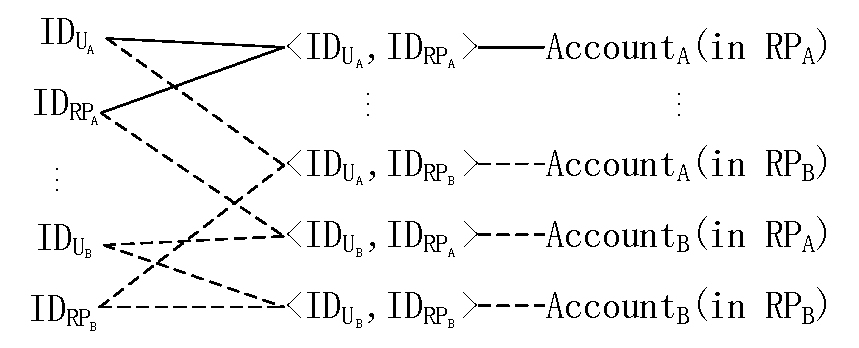
\includegraphics[width=\linewidth]{fig/link1.pdf}
  \caption{Traditional SSO.}
  \label{fig:TraditionalSSO}
\end{figure}
\begin{figure}
  \centering
  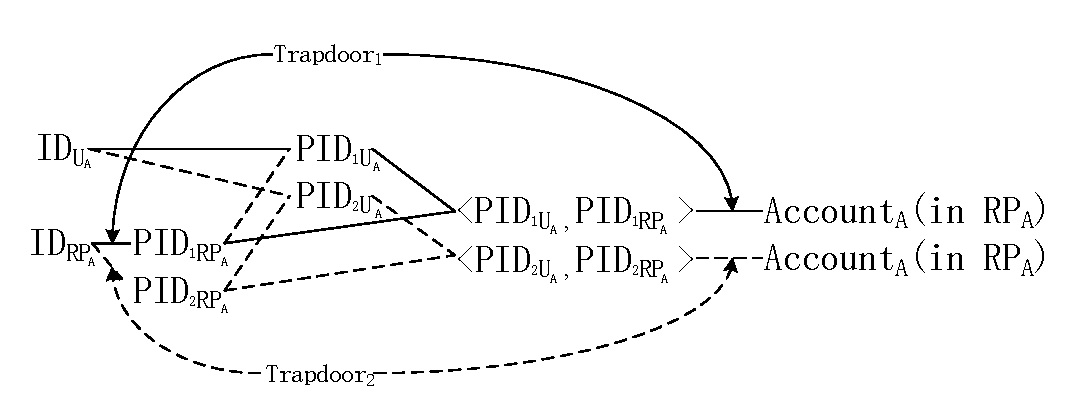
\includegraphics[width=\linewidth]{fig/link2.pdf}
  \caption{Our scheme.}
  \label{fig:Ourscheme}
\end{figure}
\begin{figure}
  \centering
  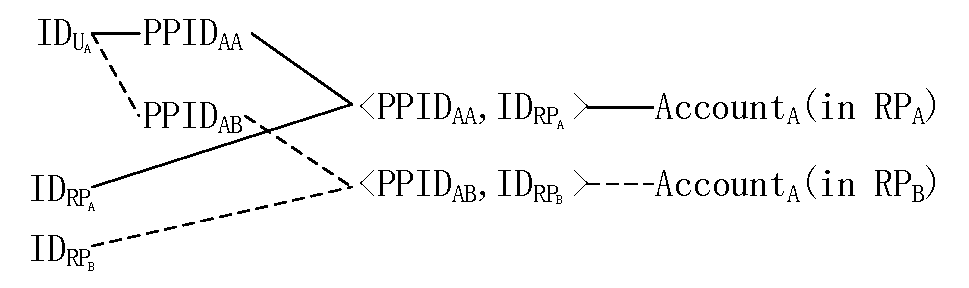
\includegraphics[width=\linewidth]{fig/link4.pdf}
  \caption{PPID.}
  \label{fig:PPID}
\end{figure}
\begin{figure}
  \centering
  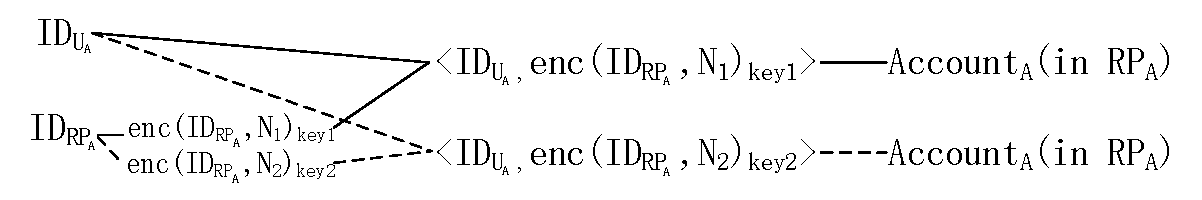
\includegraphics[width=\linewidth]{fig/link3.pdf}
  \caption{SPRESSO.}
  \label{fig:SPRESSO}
\end{figure}


%In BrowserID and SPRESSO, collusive RPs could link a user's multiple logins from the common user identifier.
%In this paper, we present UPRESSO, an Unlinkable Privacy-REspecting Single Sign-On system,
%UPRESSO, privacy-\(RE\)specting single sign-On system a\(C\)hieving un\(L\)inkable \(USE\)rs' traces
%as a comprehensive solution to tackle the privacy problems in SSO. We propose novel identifier generation schemes to dynamically generate  privacy-preserving user and RP identifiers, denoted as $PUID$ and $PRPID$, to construct identity proofs for SSO, which satisfy three properties: (1) when a same or differnt user(s) log in to a same RP, random $PRPID$s are generated in different logins so that a curious IdP cannot infer the real identity of the RP or link multiple logins at that RP; (2) when a same user logs in to a same or different RPs, random $PUID$s are generated so that
%neither a curious IdP nor
%collusive RPs cannot link the logins of that user; (3) when a same user logs in to a same RP, the RP can derive a unique user identifier from different PUIDs with a trapdoor so that it can provide a continuous service to the user during different logins.

%from both the IdP and RPs, named {UPRESSO}. To achieve this, we rely on the user to achieve the trusted transmit and correctness check of identity proof (same as in BrowserID~\cite{persona}), and propose two algorithms to achieve:

%{\color{blue} To achieve this, we propose the novel method to enable the IdP to generates the pairwise user identifier with the RP's one-time identity, which never exposes the RP's real identity. The method is consisted of RP's identifier generation and PPID generation, where two algorithms are proposed to achieve:}

\begin{comment}

\begin{itemize}
\item RP's identifier generation and transformation, which makes the RP's identifier in multiple authentications  different, and IdP fails to infer RP's information or link it in different authentications. Moreover, neither RP nor the user may control the generated identifier, which avoids the misuse of the identity proof. The detailed analysis is provided in Section~\ref{sec:analysis}.
\item PPID generation, which makes the PPIDs for one user in one RP indistinguishable from others (e.g., different users in different RPs), while only the RP (and the user) has the trapdoor to derive the unique identifier from different PPIDs for one user in one RP.
\end{itemize}

\end{comment}

%{\color{blue} Besides, we also propose a way to shift the responsibilities of trusted transmit and correctness check of identity proof from IdP to user. }


%In this paper, we propose the first scheme which deals with all the privacy issues introduced by SSO comprehensively. UPRESSO enables the RP to hide its identity from IdP for users authentication, as well as IdP is able to provide distinct user identifiers for each RP. To achieve the above goals, we  proposed the scheme for RP and user identifier generating, which allows that, 1) RP has the ability to offer the changing RP identifiers to IdP in each authentication, from which the real RP identity is not possible to be derived without the trapdoor; 2) IdP is able to generate unique user identifier (\verb+user_idp_id+) bound with specific RP identifier, from which the user identifier in RP(\verb+user_rp_id+)is to be derived with the trapdoor. However, multiple RPs are unable to link the user by \verb+user_rp_id+ or \verb+user_idp_id+.

Unlike previous approaches that require non-trivial re-design of the existing SSO systems, UPRESSO can be implemented over a widely used OIDC system with small modifications with the support of its dynamic registration function~\cite{DynamicRegistration}.

%Reluse only requires the following modification on  OIDC implementations: (1) an additional web service at the IdP for providing a  set of public parameters; (2) the support for generating  the new RP identifier (at the user and RP), PPID (at the IdP) and user's account (at RP). The prototype demonstrates  that UPRESSO is incompatible with existing OIDC implementations.

%Compared with BrowserID and SPRESSO, UPRESSO does not only deal with the privacy issues comprehensively but also be compatible with traditional OIDC system, which is not achieved by neither BrowserID and SPRESSO. BrowserID requires that the user's identity proof should be generated by user's browser, as well as SPRESSO has to introduce new trustful party into the system.
%To deal with the security considerations introduced by hiding RP in OIDC: 1) the identity proof should only be sent to the correct RP; 2) identity proof should not be misused. The following requirements should be fulfilled by UPRESSO:
%\begin{itemize}
%\item A new algorithm is proposed to negotiate the RP's identifier between the user and RP for each login. Therefore, the RP's identifier in multiple authentications are different, and IdP fails to infer RP's information or link it in different authentications. Moreover, neither RP nor the user may control the generated identifier, which avoids the misuse of the identity proof. The detailed analysis is provided in Section~\ref{sec:analysis}.
%302跳转可以不产生referer
%\item A browser extension is introduced to transmit the messages (i.e.,  request and response) related with the authentication, which ensures only the correct RP receives the id token.
%\item A new generation algorithm of PPID is provided, which makes the PPIDs for one user in one RP  indistinguishable  from others (e.g., different users in different RPs), while only the RP (and the user) has the trapdoor to derive the unique identifier from different PPIDs for one user in one RP.
%\end{itemize}
%We implement UPRESSO prototype as follows: the IdP is based on the MITREid Connect, RP is a Java web service based on the SpringMVC framework and a chrome extension for the functions on the user side. %Finally we prove the availability of the UPRESSO and evaluate the delay introduced by UPRESSO.


%In this paper, we propose an extension (named PriOIDC) of existing widely adopted SSO system (i.e., OIDC), which preserves the systematically and thoroughly analyzed security, and achieves the fully privacy. That is, (1) the security design in OIDC is inherited to prevent the impersonation attack and  identity injection attack, (2) the privacy enhance mechanisms (e.g., the clear consent from the user and the PPID) are retained, (3) a new mechanism is introduced to hide the user's accessed RP from IdP. Unlike designing and deploying a new SSO systems, we only need to analyze the compliance of the new function (i.e., hiding the user's accessed RP) and the influence to the security introduced by the new mechanism. And, the deployment of PriOIDC only requires: (1) IdP provides a set of public parameters and generates the PPID with a newly provided algorithm, (2) RP integrates the SSO service with a new version software development kit (SDK) whose interface remains unchanged, (3) the user installs an extension to access RP with full privacy anywhere as no persistent storage is required in the user side.



%Moreover, the basic requirement of SSO systems is the security, which includes two aspects: 1) the attacker should not be able to access the honest RP with the honest users' identity; 2) the identity injection will never succeed, that is, the attacker should not be able to make the honest user access the RP with an incorrect identity. Plenty of works are proposed for the security of SSO systems.
%Firstly, various standards, e.g., OAuth 2.0~\cite{rfc6749}, SAML~\cite{SAML} and OpenID Connect (OIDC)~\cite{OpenIDConnect}, are proposed to formalize the handling at each entity (i.e.,  the user, RP and IdP)  and the information exchanges between the entities.
%Secondly, the standards, SAML, OAuth and OIDC, are formally analyzed, for example, a general Dolev-Yao style web model is proposed for the web infrastructure~\cite{webmodel} and adopted to analyze the security of OAuth and OIDC~\cite{FettKS16}~\cite{FettKS17}.
%Moreover, the typical implementations of SSO systems, e.g. Google, Facebook, Twitter and the corresponding RPs, are systematically analyzed~\cite{WangCW12}~\cite{FettKS16}~\cite{ZhouE14}~\cite{WangZLG16}, which makes  the security of SSO systems improved significantly.








%整理逻辑

%第三段
%现有研究
%现有研究的缺点
%能否提供统一的隐私要求

%匿名SSO打算放到related work中



%Two SSO systems (BrowserID~\cite{persona} and SPRESSO~\cite{SPRESSO}) are proposed to hide the user's accessed RPs from IdP, while ensuring the security of SSO systems simultaneously. In BrowserID, the user is responsible for sending the identity proof correctly and binding the proof with the correct RP using a newly generated private key, while the corresponding public key is bound with the email address by the IdP who fails to obtain the information of accessed RP. In SPRESSO, the identity proof is bound with an encryption of the RP's domain name by the IdP who knows the user's identity but not the plaintext of the RP's information, and sent to the exact RP by a newly introduced trusted entity (called FWD) who obtains the RP's domain name but not the identity of the user.

%In BrowserID, the identity proof sent by the user to the RP directly, contains two parts: one is generated by the IdP which binds the user's email address with a public key, and the other is a signature of the RP generated by the user with the corresponding private key. Therefore, IdP in BrowserID fails to obtain the information of RP. In SPRESSO, RP encrypts its domain name (and a random nonce) with a symmetric key as the identifier  to obtain the identity proof, which makes others fail to infer the RP from the identifier, and a new entity (FWD) is introduced to relay the identity proof from the IdP to the RP. Therefore, for one identity proof in SPRESSO, IdP only knows the user's identity  while the FWD only knows the RP.



%However, BrowserID and SPRESSO are both redesigns of SSO systems, and therefore incompatible with existing widely deployed SSO systems (e.g., OAuth, OIDC and SAML). Moreover, the new SSO systems require a  complicated, formal and thorough security analysis of both the designs and various implementations. As shown in ~\cite{BrowserID}, vulnerabilities have been found in the implementation of BrowserID. More importantly,  in order to provide the same identity to the RP in the multiple logins of a user, both BrowserID and SPRESSO use the email address as the identity, which makes the user linkage (from multiple RPs) possible.

%Vairous SSO protocols are proposed to hide the users' accessing to RPs from the IdP. In the BrowserID system~\cite{persona}, a user firstly generates a asymmetric key pair. The IdP authenticates the user and offers a user certificate (UC) which contains the user's email address with the user's public key. User is to sign the origin of the RP with the corresponding private key as the identity assertion (IA). RP is able to identify the user by UC and IA.
%the user sends RP the user certificate (i.e. combing the user's email address with the user's public key) and identity assertion (i.e., the origin of the RP signed by the user with the corresponding private key) to complete the authentication, and is formally analyzed and found severe attacks~\cite{BrowserID}.
%SPRESSO~\cite{SPRESSO} is designed based on the standard HTML5 and web features, and formally analyzed based on the expressive Dolev-Yao style model of the web infrastructure~\cite{webmodel}. But for RPs to identify a user, both BrowserID and SPRESSO need to provide user's real identity (or a constant pseudonym) to each RP. Communication among multiple RPs would allow RPs to profile the user.
%If a user logs in multiple RPs, these RPs are able to draw his/her trace.


%Therefore there are no SSO protocols so far that protect users from tracking by both IdP and RPs simultaneously. NIST publication has issued that proxy is able to protect users' privacy in SSO system. It is defined that when the proxy can keep IdP and RP anonymous to each other and itself the proxy is called the triple blind proxy. But no existing proxy has achieved this goal.
%that the triple blind proxy can protect users from being tracked, but there is no existing systems achieved this goal.
%Moreover, the protocols protecting user's privacy (such as, SPRESSO and BrowserID) are quite distinct from the widely adopted protocols. There is to be a huge cost if IdP developers migrate their systems into a totally brand-new architecture.
%第四段
%IdP钓鱼网站问题
%转移到安全分析
%Besides tracking user, IdP in traditional SSO system is not expected to protect users from phishing attack either. Imagine that you visit \emph{phishingsite.com} which is established by a malicious opponent and allows user to log in using a Google account. Google SSO allows web application to direct user to Google's login web page and user need log in Google. However, \emph{phishingsite} directs you to a phishing site totally same as Google's web page instead of the real one. That is, while you accomplish the authentication, e.g., inputting your password, your password is to be stolen by malicious opponent.

%Phishing attack in SSO systems has been considered by OAuth 2.0~\cite{rfc6749} and several papers~\cite{anti_phishing}~\cite{devil_phishing}~\cite{mechanism_phishing} are proposed to discuss it. There is, however, no existing schemes can be adopted to enhance the security of popular protocols, e.g., OpenID Connect.


%In this paper, we propose an extension (named PriOIDC) of existing widely adopted SSO system (i.e., OIDC), which preserves the systematically and thoroughly analyzed security, and achieves the fully privacy. That is, (1) the security design in OIDC is inherited to prevent the impersonation attack and  identity injection attack, (2) the privacy enhance mechanisms (e.g., the clear consent from the user and the PPID) are retained, (3) a new mechanism is introduced to hide the user's accessed RP from IdP. Unlike designing and deploying a new SSO systems, we only need to analyze the compliance of the new function (i.e., hiding the user's accessed RP) and the influence to the security introduced by the new mechanism. And, the deployment of PriOIDC only requires: (1) IdP provides a set of public parameters and generates the PPID with a newly provided algorithm, (2) RP integrates the SSO service with a new version software development kit (SDK) whose interface remains unchanged, (3) the user installs an extension to access RP with full privacy anywhere as no persistent storage is required in the user side.

%第⑤段:
%我们的目标
%建立一套新的单点登录系统,满足:
%1 满足NIST的隐私需求
%2 便于现有系统的迁移
%To hide the user's accessed RP from IdP, PriOIDC avoids the potential leakage in the identity proof (i.e., id token in OIDC)  and the corresponding message transmission. Moreover, PriOIDC enables only the RP (and the user) to derive the user's unique identifier from different PPIDs,  which  allows the RP to provide the individual service with the unique identifier and avoids the user linkage as both the PPID and user's unique identifier in RP are different for various RPs. PriOIDC achieves these as follows:
%\begin{itemize}
%\item A new algorithm is proposed to negotiate the RP's identifier between the user and RP for each login. Therefore, the RP's identifier in multiple id tokens are different, and IdP fails to infer RP's information in the generation of one or multiple id tokens. Moreover, neither RP nor the user may control the generated identifier, which avoids the misuse of the id token. The detailed analysis is provided  in Section~\ref{sec:analysis}.
%\item A browser extension is introduced to transmit the messages (i.e.,  request and response) related with the id token. IdP fails to infer the RP's information through the network traffic, and the extension ensures only the correct RP receives the id token.
%\item A new generation algorithm of PPID is provided, which makes the PPIDs for one user in one RP  indistinguishable  from others (e.g., different users in different RPs), while only the RP (and the user) has the trapdoor to derive the unique identifier from different PPIDs for one user in one RP.
%\end{itemize}


%第六段
%我们的贡献
%提出协议
%考虑能否根据模型进行分析
%实现原型系统
The main contributions of UPRESSO are as follows:
\begin{itemize}
\item We systematically analyze the privacy issues in SSO systems and propose a comprehensive protection solution to hide users' traces from both curious IdPs and collusive RPs, for the first time. We also provide a systematic analysis to show that UPRESSO achieves the same level of security as existing SSO systems.
%deals with all the privacy issues introduced by SSO comprehensively. It has the ability to prevent IdP from tracking users' login trace, as well as multiple RPs are unable to link the users either.
%pratical extension for OIDC, which inherits the systematically and thoroughly analyzed  security and privacy mechanisms of OIDC, and achieves the full privacy for users by hiding the accessed RPs from IdP.
\item We develop a prototype of UPRESSO that is compatible with OIDC and demonstrate its effectiveness and efficiency with experiment evaluations.
\end{itemize}



%第七段
%文章结构
The rest of this paper is organized as follows. We introduce the background in Sections~\ref{sec:background}, and the challenges with solutions briefly~\ref{sec:challenge}. Section~\ref{sec:related} and Section~\ref{sec:UPRESSO} describe the threat model and the design of UPRESSO. A systematical analysis is presented in Section~\ref{sec:analysis}. We provide the implementation specifics and evaluation in Section~\ref{sec:implementation}, then introduce the related works in Section~\ref{sec:related}, and draw the conclusion finally.
% and Section~\ref{sec:evaluation}

%This paper is organized as follows: Section~\ref{sec:back} provides the knowledge of OpenID Connect. Section~\ref{sec:overview} gives the overview of this scheme and its attack surface. Section~\ref{sec:protocol} describes the construction and details of this scheme. Section~\ref{sec:analysis} provides the detailed analysis of the new scheme. Section~\ref{sec:evaluation} offers a performance evaluation of our prototype system. Section~\ref{sec:related} discusses the related works. In Section~\ref{sec:conclusion}, a conclusion is given.



\begin{comment}
%These protocols are classified into two classes according to the objective:
%(1) preventing the RP obtaining the user's identity and (2) avoiding the IdP learning at which RP the user logins in.
Anonymous SSO authentications schemes belonging to the first one and apply to the RPs who do not require the user's identity nor PII, and just  need to check whether the user is authorised or not. These schemes allow users to access a service protected by a verifier without revealing their identities to the RPs.

However, to provide the continuous and preconized service, RP needs to obtain the unique pseudonym for each user.
In this case, the solutions belong to the class 2 is more suitable, as the IdP doesn't know which RP the user access while the RP only knows the user's pseudonym but not the real identity.
Vairous SSO protocols are proposed to hide the users accessed RPs from the IdP.
In the BrowserID system~\cite{persona}, the user sends RP the user certificate (i.e. combing the user's email address with the user's public key) and identity assertion (i.e., the origin of the RP signed by the user with the corresponding private key) to complete the authentication, and is formally analyzed and found severe attacks~\cite{BrowserID}.
SPRESSO~\cite{SPRESSO} is proposed based on the standard HTML5 and web features, and formally analyzed based on the expressive Dolev-Yao style model of the web infrastructure~\cite{webmodel}.





For security consideration, the ticket issued by the IdP should contain the identity of RP, to send the ticket or ticket index, the IdP should construct the rediect URL which contains the  RP URL.

%大量工作来提升协议的安全性,包括1.协议本身的安全性;2. 具体实现的安全性。
The security of SSO systems is improved by .
The OAuth 2.0 and OpenId-Connect protocol are formally analyzed under the web model.
The implementations have been evaluated and various vulnerabilities are found which
%Authentication is the first line to protect the user information,

%SSO引入了新的隐私问题,目前已有多项工作1. 协议规范要求IdP在向RP传输PII时,需要得到用户明确授权;2.用户在不同RP使用的不同的标识,防止串联 3.匿名SSO,防止RP获取用户信息


%但是SSO引入了一个明显的问题,即IdP将获取用户访问的RP信息,从而能够***


%本文提出了一种匿名方案,通过集成***,实现了。可以描述该工作的难点





A Single Sign-On (SSO) system contains Identity Provider (IdP), Relying Parties (RP) and users. It allows users to log in the IdP once and then user can use RPs' service without extra login. Currently internet services have been an essential part of people's life. To provide their users with personalized services, many web application developers manage to authenticate users. Traditional authentication system requires users to keep individual accounts and passwords.

%SSO引入了新的安全问题 However, SSO introduces new risk to the user's privacy.
Introduce the flaws of current sso system. All the popular sso protocols can't hide the login information , who login in which web application. And even the specification of some protocols advise the IdP should keep the user identity unique in each RP, but may sso service providers haven't confirm the rule, such as Google.

%现有的缓解方法
Introduce what we want about the sso system. When the user logs in a RP with the sso service, the IdP will get nothing can link the user an the RP. And even the multi-RP collusion cannot deduces the user's login trace.

%但是现有解决方法还不够,引入我们的问题
Our contributions:

%我们方法的基本原理

\end{comment}

\section{Background}
\label{sec:background}
Recluse aims to preserve the users' privacy by hiding the users' traces from both IdP and RPs in SSO systems (e.g., the widely adopted OIDC SSO systems), with the security of SSO systems under consideration. This section adopts OIDC as the example to present the necessary background information  and the security consideration of SSO sytems.

%Recluse is an extension of OIDC to prevent the IdP from inferring the user's accessed RP, with the security of SSO systems under consideration.
%provides the necessary background information about OIDC and  the security consideration of SSO systems.
%Most of current IdPs\cite{Facebook} for web application use OAuth 2.0 authorization code flow. Because authorization code flow requires RP's secret for token exchanging. It actually achieves the binding of RP and access token. Although OAuth 2.0 implicit flow is not secure in authentication, many IdPs also use its modified version designed by each IdP for authentication.
%In this section, we firstly describe how OpenID Connect is defined. Then the discussion of SSO system is to illustrate that why OpenID Connect is chosen and the challenges and solutions of protecting user's privacy.

\subsection{OpenID Connect}
\label{subsec:OIDC}
Typical SSO systems~\cite{SAMLIdentifier,OpenIDConnect,SPRESSO} contain the following entities:
%The OIDC or OAuth systems contains following entities:
\begin{itemize}
    \item \textbf{IdP}. IdP maintains the user's attributes and credentials, performs the user authentication, generates the identity proof with its private key, binds it with the RP and sends the poof (or the reference) to the correct RP through the user. The generation of identity proof is processed differently in various SSO systems. For example, in OIDC, IdP generates a PPID for the user's first login at a RP, checks the consistency of the RP's information (the URL and identifier) between ones from the maintained database and the request, and requires the  consent from the user about the exposed attributes.
     \item \textbf{User}. This entity completes the authentication at the IdP with securely maintained credentials, initiates a SSO process by requiring to login at a RP, relays the identity proof request from the RP to IdP, checks the scope of attributes exposed to RP, and transmits the identity proof (or the reference) from IdP to the RP correctly. Usually, these processes are handled by  a user-controlled software (e.g., the browser), called user agent.
    \item \textbf{RP}. RP provides the individual services based on the identifier (i.e., account) from the identity proof. In details, RP constructs the identity proof request, sends the request to the IdP through the user, checks the correctness of the received identity proof, and parses the proof for necessary information. The details process varies in different systems. For example, in OIDC, RP needs to register at the IdP for the identifier to be used in the construction of the identity proof request, and derives the user's account based on PPID.
\end{itemize}
\begin{comment}
\begin{itemize}
    \item \textbf{User}. is the entity to be authenticated in this system who holds the credentials for the IdP. User takes part in the the system through the user agent. User agent is the software used by the user, such as browser and the application on the mobile device, which is required to transmit the authentication request and identity proof between IdP and RP correctly.
     \item \textbf{IdP}. is the entity who authenticates the user and provide the identity proof. IdP authenticates the user, verifies the authentication request from RP, generates user's PPID and issues the identity proof signed with its private key. Besides, IdP provides the notification to user about the range of exposed attributes to RP and guarantees that the identity proof should only be sent to the corresponding RP.
    \item \textbf{RP}. is the entity who provides the service and need to identify the user. RP builds the authentication request to IdP with its identifier and endpoint for identity proof. RP identifies a user through the PPID in identity proof.
\end{itemize}
\end{comment}


OpenID Connect (current version 1.0), a typical SSO standard,  defines the process at each entity and the protocol flows between entities. OIDC is  an extension of OAuth (current version 2.0). OAuth is originally designed for authorizing the RP to obtain the user's personal protected resources stored at the resource holder. That is, the RP obtains an access token generated by the resource holder after a clear consent from the user, and  uses the access token to obtain the specified resources of the user from the resource holder. However, plenty of RPs adopt OAuth 2.0 in the user authentication, which is not formally defined in the specifications~\cite{rfc6749,rfc6750}, and makes impersonation attack possible~\cite{ChenPCTKT14, WangZLG16}. For example, the access token isn't required to be bound with the RP, the adversary may act as a RP to obtain the access token and use it to impersonate as the victim user in another RP.

%OpenID Connect (current version 1.0) is an extension of OAuth (current version 2.0). OAuth is originally designed for authorizing the RP to obtain the user's personal protected resources stored at the resource holder. That is, the RP obtains an access token generated by the resource holder after a clear consent from the user, and  uses the access token to obtain the specified resources of the user from the resource holder. However, plenty of RPs adopt OAuth 2.0 in the user authentication, which is not formally defined in the specifications~\cite{rfc6749,rfc6750}, and makes impersonation attack possible~\cite{ChenPCTKT14, WangZLG16}. For example, the access token isn't required tp be bound with the RP, the adversary may act as a RP to obtain the access token and use it to impersonate as the victim user in another RP.


%OAuth 2.0 is specifically designed for user authorization. It allows third party to access user's personal protected resources from resource holder. In OAuth 2.0 system everyone carrying user's access token is able to achieve user's protected resources from resource holder. Access token is not bound with any RP so that it is not appropriate for authentication. OpenID Connect offers an additional id token for user identifying so that it can be used in both authentication and authorization.

%OpenID Connect 1.0 is an extension of OAuth 2.0. OAuth 2.0 is specifically designed for user authorization. It allows third party to access user's personal protected resources from resource holder. In OAuth 2.0 system everyone carrying user's access token is able to achieve user's protected resources from resource holder. Access token is not bound with any RP so that it is not appropriate for authentication. OpenID Connect offers an additional id token for user identifying so that it can be used in both authentication and authorization.

OIDC is designed to extend OAuth for user authentication by binding the identity proof for authentication with the information of RP. OIDC provides three protocol flows: authorization code flow, implicit flow and hybrid flow (i.e., a mix-up of the previous two flows). In the authorization code flow, the identity proof is the authorization code sent by the IdP, which is bound with the RP, as only the target RP is able to obtain the user's attributes with this authorization code and the corresponding secret (distributed in the RP's registration).

The implicit flow of OIDC achieves the binding between the identity proof and the RP, by introducing a new token (i.e., id token). In details, id token includes the user's PPID (i.e., \verb+sub+), the RP's identifier (i.e., \verb+aud+), issuing time, the validity period and the other requested attributes. The IdP completes the construction of the id token by generating the signature of these elements with its private key, and sends it to the correct RP through the redirect URL registered previously.  The RP validates the id token, by verifying the signature with the IdP's public key, checking the correctness of the valid period and the consistency of \verb+aud+ with the identifier stored locally. Figure~\ref{fig:OpenID} provides the details in the implicit flow of OIDC, where the dashed lines represent the message transmission  in  the browser while the solid lines denote the network traffic. The detailed processes are as follows:
\begin{itemize}
    \item Step 1: User attempts to login at one RP.
    \item Step 2: The RP redirects the user to the corresponding IdP with a newly constructed request of id token. The request contains RP's identifier (i.e., \verb+client_id+), the endpoint (i.e., \verb+redirect_uri+) to receive the id token, and the set of requested attributes (i.e., \verb+scope+). Here, the \verb+openid+ should be included in \verb+scope+ to request the id token.
    \item Step 3: The IdP generates the id token and the access token for the user who has been authenticated already, and constructs the response with  endpoint (i.e., \verb+redirect_uri+)  in request if it is the same with the registered one for the RP. If the user hasn't been authenticated, an extra authentication process is performed.
    \item Step 4, 5: The RP verifies the id token, identifies the user with \verb+sub+ in the id token, and requests the other attributes from IdP with the access token.
\end{itemize}
\begin{figure}
  \centering
  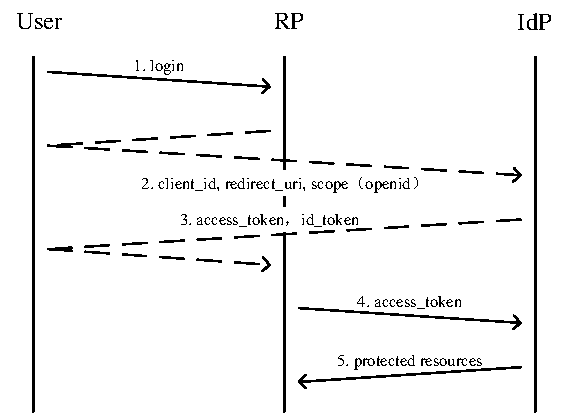
\includegraphics[width=0.8\linewidth]{fig/implicit.pdf}
  %\subfigure[Authorization Code Flow]{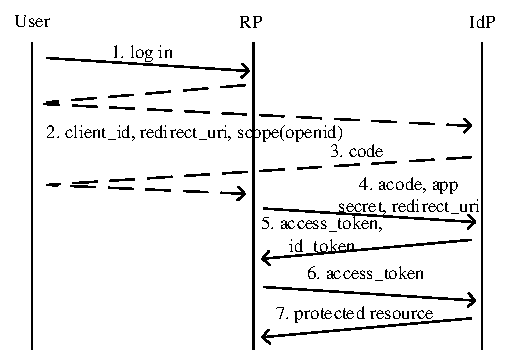
\includegraphics[width=\linewidth]{fig/openidconnect2.pdf}\label{fig:OpenID_code}}
  %\subfigure[Hybrid Flow]{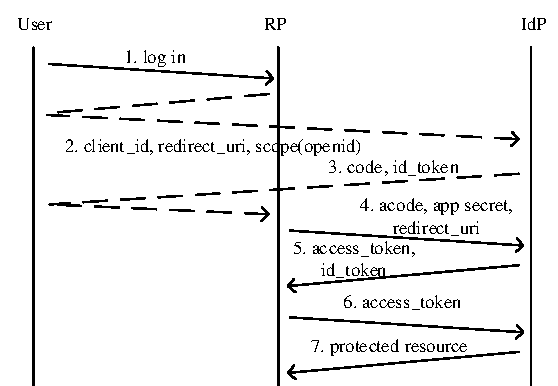
\includegraphics[width=\linewidth]{fig/openidconnect3.pdf}\label{fig:OpenID_hybrid}}
  \caption{The implicit protocol flow of OIDC.}
  \label{fig:OpenID}
\end{figure}

\noindent\textbf{Dynamic Registration.} The id token (also, the authorization code) is bound with the RP's identifier (i.e., \verb+client_id+). OIDC provides the dynamic registration~\cite{DynamicRegistration} mechanism to register the RP for a new \verb+client_id+, dynamically. After the first successful registration, RP obtains a registration token from the IdP, and is able to update its information (e.g., the \verb+redirect URI+ and the  response type) by a dynamic registration process with the  registration token. One successful dynamic registration process  will make the IdP assign a new unique \verb+client_id+ for this RP.

\subsection{Security Consideration}
\label{subsec:securityconsideration}
As described in~\cite{SPRESSO}, the design of SSO systems is challenging, as the adversary may adopt various attacks~\cite{ChenPCTKT14, FettKS16, WangCW12, WangZLG16, ZhouE14, rfc6819, YangLLZH16} to achieve:
\begin{itemize}
\item Impersonation attack: Adversaries login to a RP as the victim user. Then, the adversary obtains the full control of user's account in the RP, and behaves arbitrarily under the victim's identity.
\item Identity injection: Honest user logins to a RP with the adversaries' identity. Then, the privacy of the victim users may be leaked. For example, the victim user may upload the private data to the OneDrive or iCloud under the adversary's account.
\end{itemize}

To prevent impersonation attack and identity injection, SSO systems are designed and analysed with the following security considerations. In details, in addition to being bound with the correct user, which is the basic requirement of authentication,  the identity proof should satisfy the following requirements:
\begin{itemize}
    \item \textbf{Confidentiality.} The identity proof should only be obtained by the correct RP (and the user), no one else may get the identity proof~\cite{ChenPCTKT14,FettKS16,WangZLG16}. Otherwise, the adversary may use the obtained identity proof to login as the victim user on the specified RP. To avoid the unauthorized leakage of identity proof, (1) the  user and IdP should perform additional checks  in its generation and transmit to ensure that the identity proof is generated for the correct RP (i.e., the correct identifier) and sent to the exact RP (i.e., correct URL); (2) TLS is adopted to ensure the confidentiality during transmit; (3) a trusted user agent is deployed to ensure the identity proof is only sent to the URL specified by the IdP.
    \item  \textbf{Integrity.} The valid identity proof should only be generated by the IdP, no one else may forge or modify a valid proof~\cite{WangZLG16}. Otherwise, the adversary may replace the user's identifer in the proof for either impersonation attack and identity injection. To ensure the integrity of identity proof, (1) the signature is required for each identity proof using the unleaked private key of IdP; (2) the RP should check the signature correctly, and only accept the information protected by the signature, as the others may be tampered. (add reference such as the SAML attacks).
    \item  \textbf{Binding.} The identity proof should be bound with only one RP and accepted only by this RP, no other honest RP may accept this identity proof. Otherwise, the adversary may impersonate as the victim user, for example, by pretending as a RP to collect the victim's identity proof and using it at any other honest RP. To ensure the correct binding, (1) IdP should include the RP's identifier in the proof and adopt the signature to avoid the modification, (2) RP should checks the consistency between its identifier with the one in the identity proof. (add  attack reference)
    %, and the honest RP checks the consistency of the identifier in the id token with the one stored locally.
\end{itemize}

In addition to the above security considerations, some other conventional checks are required in the RP to ensure the security. For example, the identity proof should be considered valid only in the specified period; the replayed identity proof needs to be rejected.

Beside the security, the privacy is also considered in SSO systems. For example, the user should be able to control the range of attributes exposed to the RP, which is achieved by one extra user's consent required by IdP.

\subsection{Primitive Root}
\label{subsec:primitive}
A number $g$ ($0<g<P$) is called a primitive root modular a prime $P$, if for ${\forall}y$ ($0<y<P$), there is a (unique) number $x$ ($0\le x <P-1$) satisfying $y=g^x \pmod P$. Here, $x$ is called the discrete logarithm of $y$ modulo $P$. Given a large prime $P$ and a number $y$, it is computationally infeasible to derive the discrete logarithm (here $x$) of $y$ (detailed in~\cite{WXWM}), which is called  Discrete Logarithm Problem. The hardness of solving discrete logarithm has been a base of the security of several security primitives, including
Diffie-Hellman key exchange and Digital Signature Algorithm. 

To calculate the primitive root for a given large prime $P$,  we first search the least primitive root $g_m$  mod $P$, and then calculate the primitive root $g = g_{m}^{t} mod \ P$, where $t$ is an integer coprime to $P-1$.
We checks whether a integrity $\mu$ is the primitive root modulo $P$ where $P=2Q+1$ ($Q$ is a prime), based on the lemma that an integer $1<\mu <P-1$ is a primitive root if and only if $\mu^2\neq 1 \pmod P$ and $\mu^Q\neq 1 \pmod P$.
The details are provided in~\cite{Shoup,Wang}.



\begin{comment}
It is a classical result that for any prime number $P$, there is a number $0<g<P$
such that $g$ is a primitive root mod $P$ in the sense that: given a number $0<y<P$, there is
a (unique) number $0\le x <P-1$ such that $y=g^x \pmod P$. One usually writes $x=\log_g y$ and
calls $x$ the discrete logarithm of $y$ modulo $p$. If we denote ${\mathbb F}_P$ the finite field
$\{0, 1, \cdots, P-1\}$ and let $\mathbb{F}_P^*=\{1, \cdots, P-1\}$, then
${\mathbb F}_P^*$ is a cyclic group (under multiplication mod $P$) with $g$ being a generator.

Assume the prime $P$ has the form $P=2q+1$ with $q$ being a large prime, then given $y\in {\mathbb F}_P^*$, finding its
discrete logarithm $x$ is computationally infeasible. This is because the order of $g$ (which is $2q$) has a large prime factor.
The hardness of solving discrete logarithm has been a base of the security of several security primitives, including
Diffie-Hellman key exchange and Digital Signature Algorithm. See \cite{WXWM} for more detail.

Under our assumption, an integer $1<\mu <P-1$ is a primitive root if and only if
$\mu^2\neq 1 \pmod P$ and $\mu^q\neq 1 \pmod P$. Usually we choose $g$ to be the least primitive root mod $P$. There
Some algorithms for searching the least primitive root mod $P$ (under
the Extended Riemann Hypothesis) can be found in \cite{Shoup,Wang}.

It is easy to verify that for any integer $1\le t <P-1$ with $\gcd(t, P-1)=1, \ g^t\pmod P$ is also a primitive root.
\end{comment}

\begin{comment}
It has been described in~\cite{SPRESSO} that in SSO systems, an adversary tries to break the authentication security in following ways:
\begin{itemize}
\item Impersonation Attack: Adversaries login to the honest RP as the honest user.
\item Identity Injection: Honest user logsin to the honest RP under adversaries' identity.
\end{itemize}
It is proved by the analysis of current widely deployed SSO systems ~\cite{ChenPCTKT14, FettKS16, WangCW12, WangZLG16, ZhouE14, rfc6819, YangLLZH16} as the attacks on the authentication illustrated in these works should be classified into these two categories.


The impersonation attack allows the adversary obtain the full control of user's account in the RP so that adversary has the ability to do anything it wants in the identity of the user. The identity injection leads the honest user log in an honest RP in the identity of the adversary which might leak the privacy of the user, for example, the user might log in the file hosting service such as OneDrive or iCloud as the adversary unconsciously and uploads the personal files to the adversary's account. To deal with the threat of the adversary, widely deployed SSO systems, such OIDC, are designed with the following security considerations, and various implementations of IdP and RP are also analysed with the same security principles under the assumption that IdP is trusted. Here, we list the security considerations:
\begin{itemize}
    \item \textbf{Content Checking: }The contents in the identity proof are generated under a clear consent of the user. The contents include the RP's information and the range of exposed attributes. For example, it has been described in~\cite{ChenPCTKT14} that the content checking provides a way for user to check the identity of the RP which is able to avoid the leaking of user's authentication information. It can be utilized by the adversary while the Binding (described later) is also broken to obtain the user's identity proof which makes the impersonation attack possible.
    \item \textbf{Confidentiality: }The confidentiality of the identity proof is ensured, that is, only the target RP obtains the identity proof which will never be leaked by the honest RP. The HTTPS connection is used to protect the identity proof between the IdP and the user, while the trusted user agent (e.g., the browser) ensures the identity proof only sent to the correct URL (of RP) which is confirmed by the user and the IdP. For example, it has been illustrated in~\cite{ChenPCTKT14, FettKS16} the SSO systems must transmitted the identity proof to the corresponding RP and illustrated in~\cite{WangZLG16} that teh transmission must be protected by various ways such as TLS. Otherwise, it also results the leakage of user's identity proof.
    \item  \textbf{Integrity: }No one except the IdP is able to construct a valid identity proof. And any modification in the identity proof makes the identity proof invalid. The analysis in ~\cite{WangZLG16} claims that the identity proof in SSO systems must be the private and unforgeable information provided by the IdP to avoid the impersonate attack. It is also required that the identity proof should not be tampered during transmission to avoid the identity injection.
%, as only the IdP has the private key to generate a valid signature for the id token.
%Any modification in the identity proof makes the identity proof invalid.
    \item  \textbf{Binding: }The identity proof is only valid for the target RP, as it is bound with only the target RP, and the honest RP has the ability to verify the consistency. It has been described in Section~\ref{sec:introduction} that the binding of RP and identity proof avoid the adversary to use the identity proof of an honest user received by the corrupted RP to log in other honest RPs (impersonation attack).
    %, and the honest RP checks the consistency of the identifier in the id token with the one stored locally.
\end{itemize}
\end{comment}
\begin{comment}
Widely deployed SSO systems, such OIDC, are designed with the following security considerations, and various implementations of IdP and RP are also analyzed with the same security principles under the assumption that IdP is trusted. Here, we list the security considerations:
\begin{itemize}
    \item \textbf{Content Checking: }The contents in the identity proof are generated under a clear consent of the user. The contents include the RP's information and the range of exposed attributes.
    \item \textbf{Confidentiality: }The confidentiality of the identity proof is ensured, that is, only the target RP obtains the identity proof which will never be leaked by the honest RP. The HTTPS connection is used to protect the identity proof between the IdP and the user, while the trusted user agent (e.g., the browser) ensures the identity proof only sent to the correct URL (of RP) which is confirmed by the user and the IdP.
    \item  \textbf{Integrity: }No one except the IdP is able to construct a valid identity proof.
%, as only the IdP has the private key to generate a valid signature for the id token.
Any modification in the identity proof makes the identity proof invalid.
    \item  \textbf{Binding: }The identity proof is only valid for the target RP, as it is bound with only the target RP, and the honest RP has the ability to verify the consistency.
    %, and the honest RP checks the consistency of the identifier in the id token with the one stored locally.
\end{itemize}
\end{comment}

\begin{comment}
*However, the privacy considered in these works is the protected resources held by the IdP which is not necessary in authentication.
Besides, the adversary also has the interests in users' login traces, the private issue introduced by SSO systems described in Section~\ref{sec:introduction}. To undermine a user's privacy,
the adversary tries to achieve the following goals:
\begin{itemize}
\item Adversary finds out which RP a user has accessed by acting as the honest IdP.
\item Adversary links the same user in multiple RPs controlled by adversary.
\end{itemize}
\end{comment}

%OpenID Connect enables RP to verify the identity of a user based on the authentication performed by IdP. As OpenID Connect can be used in both authentication and authorization, it provides three kinds of credentials for the authentication response, containing \emph{code, token, id\_token}. \emph{Code} and \emph{token} is defined in OAuth 2.0 and \emph{id\_token} is offered only by OpenID Connect. %\emph{Code} and \emph{token} is usually used in authorization and \emph{id\_token} is used in authentication.
%The credential chosen is decided by the response\_type value in authentication request. According to the different choices of response\_type value, the use of OpenID Connect protocol can be classified as three flows: Authorization Code Flow, Implicit Flow and Hybrid Flow. The relation of response\_type and flow type is showed in table~\ref{tab:relation}

\begin{comment}

\begin{table}
\caption{OpenID Connect response\_type Values }
\begin{tabular*}{\linewidth}{@{\extracolsep{\fill}}ll}
\toprule
Response\_type Value& Flow\\
\hline
code& Authorization Code Flow\\
id\_token& Implicit Flow\\
id\_token token& Implicit Flow\\
code id\_token& Hybrid Flow\\
code token& Hybrid Flow\\
code id\_token token& Hybrid Flow\\
\bottomrule
\label{tab:relation}
\end{tabular*}
\end{table}

\noindent{\textbf{Implicit Flow.}} OpenID Connect implicit flow is shown in Figure~\ref{fig:OpenID}. All dashed lines in the figure represent the redirection by browser and solid lines represent direct network calls. Parameters on lines are important data transmitted during this call.

The OpenID Connect implicit flow is described as following steps:
\begin{itemize}
    \item Step 1: User tries to log in RP.
    \item Step 2: RP constructs token request and redirects user to IdP. Client\_id represents RP's identity, redirect\_uri represents the RP's address waiting for token and scope represents the permissions RP required from IdP. In OpenID Connect protocol, scope must contain \emph{openid}.
    \item Step 3: If IdP has authenticated user it is going to redirect user's authentication response. As response\_type requires \emph{token, id\_token}, IdP's response contains access\_token and id\_token. RP can identify a user by id\_token.
    \item Step 4, 5: RP is able to obtain user's protected resource from IdP by access\_token.
\end{itemize}
\begin{figure}
  \centering
  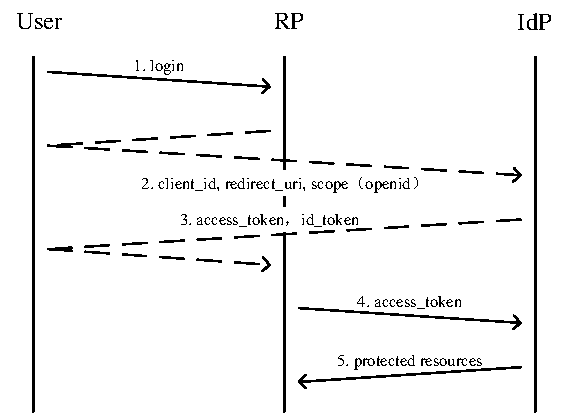
\includegraphics[width=\linewidth]{fig/implicit.pdf}\label{fig:OpenID}
  %\subfigure[Authorization Code Flow]{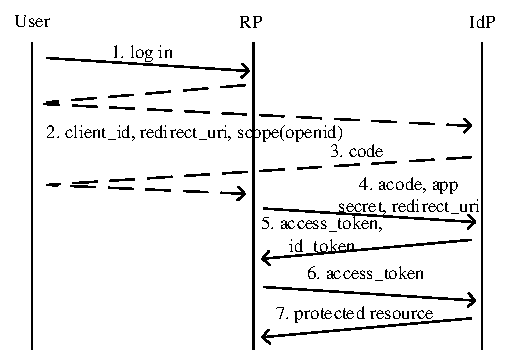
\includegraphics[width=\linewidth]{fig/openidconnect2.pdf}\label{fig:OpenID_code}}
  %\subfigure[Hybrid Flow]{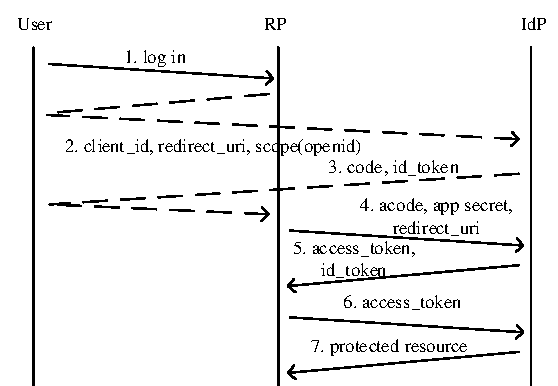
\includegraphics[width=\linewidth]{fig/openidconnect3.pdf}\label{fig:OpenID_hybrid}}
  \caption{The implicit protocol flow in OIDC.}
  \label{fig:OpenID}
\end{figure}

%Other Flows. Authorization code flow is similar to implicit flow. IdP firstly sends RP the authorization code instead of tokens. Then RP need use the code and a secret shared by RP and IdP to exchange for tokens with IdP. Hybrid flow is the combination of implicit flow and authorization code flow. RP is able to obtain code and token from IdP at the same time.
\end{comment}
\begin{comment}
\subsection{Security Consideration}
An RP must register a unique ID at IdP. To protect users' privacy, IdP should receive user's consent for specific RP before sending the PII to this RP. So IdP must get a valid ID from RP to represent RP's identity. And it has been discussed that the id token must be bound to the specific RP to avoid the reuse of token. It also requires that RP should provide the ID to IdP.

The redirect\_uri registered at IdP can avoid a malicious opponent to get a user's id token. IdP compares the redirect\_uri in the authentication request and uploaded during registration. Only when the redirect\_uri in the authentication has been uploaded during registration IdP is going to send the id token to requester. It guarantees that only the owner of the registered redirect\_uri is able to receive the id token issued for its registrant.


\subsection{Dynamic Registration}
Dynamic registration\cite{DynamicRegistration} is a function IdP provides RP to re-register its information at IdP. For dynamic registration, IdP issues each RP a registration token when the first registration of RP is finished. RP is able to register a new ID and redirect uri at IdP using the registration token.

To register a new RP at the IdP, firstly RP sends an HTTP POST message to the IdP with the parameters containing redirect uri, response type and other metadata parameters. This message is sent with the registration token. Upon successful registration, IdP generates a unique client id and returns it back with other registered metadata parameters.
\end{comment}


%流程

\begin{comment}
%\subsubsection{Analysis of OpenID Connect Flows}
%In OpenID Connect system, IdP is always able to get a user's login trace as it need to sign a id token with RP's id and user's id in it. Nist Special Publication 800-63C\cite{NIST} proposes that a user using the same IdP to authenticate to multiple RPs allows IdP to build a profile of user transactions.

%OpenID Connect 1.0 protocol is designed as extension protocol of OAuth 2.0 protocol. It can be seemed as an OAuth authentication version protocol. When OAuth protocol is firstly created there are other authentication protocols such as OpenID. So OAuth is specifically designed for user authorization. It allows third party to access user's personal protected resources from resource holder. Different from OpenID Connect 1.0, OAuth 2.0 usually offers two kinds of response type, code and token. In OAuth 2.0 protocol everyone carrying user's access token is able to achieve user's protected resources from resource holder. Access token is not bound with any RP so that it is not appropriate for authentication. It has been described in many works\cite{rfc6819}\cite{ChenPCTKT14}.
%Most of current IdPs\cite{Facebook} for web application use OAuth 2.0 authorization code flow. Because authorization code flow requires RP's secret for token exchanging. It actually achieves the binding of RP and access token. Although OAuth 2.0 implicit flow is not secure in authentication, many IdPs also use its modified version designed by each IdP for authentication.

%As OpenID Connect 1.0 is designed as an OAuth authentication version protocol, it can be used in both authentication and authorization. Id token is a security token that contains claims about authentication of a user for specific RP and it is represented as a JSON Web Token\cite{rfc7519}. In OpenID Connect 1.0 access token is mostly used for authorization. Id token is enough for user authentication. Code provides the benefit of not exposing id tokens to any malicious applications able to access user agent. Our protocol considers browser as the trust base so that authorization code flow is not necessary. We finally choose OpenID Connect 1.0 implicit flow with only response value of id\_token as the base of our enhanced protocol.

\subsection{Discussion of SSO System}
%OpenID Connect 1.0 protocol is designed as extension protocol of OAuth 2.0 protocol. When OAuth protocol is firstly created there are other authentication protocols such as OpenID. So OAuth is specifically designed for user authorization. It allows third party to access user's personal protected resources from resource holder. In OAuth 2.0 system everyone carrying user's access token is able to achieve user's protected resources from resource holder. Access token is not bound with any RP so that it is not appropriate for authentication.
%Most of current IdPs\cite{Facebook} for web application use OAuth 2.0 authorization code flow. Because authorization code flow requires RP's secret for token exchanging. It actually achieves the binding of RP and access token. Although OAuth 2.0 implicit flow is not secure in authentication, many IdPs also use its modified version designed by each IdP for authentication.

%为什么遵循openid connect,安全性得到了保证,已经被广泛使用
The reasons our privacy respecting single-sign-on protocol is designed based on OpenID Connect includes two main factors: 1) OpenID Connect 1.0 protocol and OAuth 2.0 protocol has been analysed in many previous works and they have been certified secure\cite{FettKS16}. So if the enhanced protocol can be insured as secure as OpenID Connect 1.0 protocol, it is deemed to be secure. 2) Current IdPs mostly use OAuth 2.0 and OpenID Connect 1.0 for user authentication\cite{Facebook}\cite{Google}. So it is convenient for developers to transfer their old system into the system with enhanced protocol if new protocol is similar with the previous one.

As OpenID Connect 1.0 is designed as an OAuth authentication version protocol, it can be used in both authentication and authorization. Id token is a security token that contains claims about authentication of a user for specific RP and it is represented as a JSON Web Token\cite{rfc7519}. In OpenID Connect 1.0 access token is mostly used for authorization. Id token is enough for user authentication. Code provides the benefit of not exposing id tokens to any malicious applications able to access user agent. Our protocol considers browser as the trust base so that authorization code flow is not necessary. We finally choose OpenID Connect 1.0 implicit flow with only response value of id\_token as the base of our enhanced protocol.

%单点登录系统中,IdP通过用户认证识别用户身份,通过client_id和redirect_uri识别RP身份。
%在不改变单点登录系统结构的情况下,由于IdP要向RP提供用户的身份信息,所以向IdP隐藏用户身份是不可行的
%向IdP隐藏RP身份要通过隐藏client_id和redirect_uri实现
%The ability of IdP. Discribe the solution of protecting users' privacy.
In OpenID Connect implicit flow, IdP gets a user's login trace in two ways. IdP gets RP's identity by client\_id and reditrct\_uri in redirect request (step 2) from RP. And IdP gets user's identity when authenticating the user (step 3). As IdP has to provide RP a user's authenticator bound with user's identity, it's not possible to keep user anonymous in IdP without modifying the structure of current SSO system. So it is only feasible to protect user's privacy by keeping RP anonymous in IdP. So it is needed to make client\_id and redirect\_uri unrelated with RP. But it introduces new challenges.

\subsubsection{Challenges}
%最直接的隐藏RP的方法是在登录过程中使用随机的client_id与redirect_uri
%简单的修改会带来两个方面的问题:流程问题与安全问题
%流程问题:IdP只识别注册过的client_id与redirect_uri;client_id与uid绑定,随机的client_id使每次的uid都不同
%安全问题:随机的client_id导致了不同RP之间的token可以混用;随机的redirect_uri导致IdP无法保证token只发送给对应的RP
%Security problems. The secure rules of sso system summarized from the previous research. And the simple solution will disobey which rules.
%Function problems. How the simple solution make the sso system failed.
%描述为何不能用户匿名
The simplest way to make RP anonymous in IdP is using random client\_id and redirect\_uri during each login. But the simple method will introduce some problems in two fields.

%关键句子表明问题的分类
Using random client\_id and redirect\_uri results in failure of authentication in current SSO system. IdP only accepts a request when the client\_id and redirect\_uri have been registered at IdP by an RP. So when using a random client\_id and redirect\_uri in a request, IdP will drop it as an invalid request. Additionally to protect user's privacy from RPs' collusion, it's required that IdP should provide different user\_ids for different client\_ids\cite{OpenIDConnect}. As a result, user\_id is bound to client\_id. While client\_id changing, user\_id changes. So a random client\_id for a RP means the user\_id is random too. If RP wants to provide a user personalize service user has to own a constant identity in RP. So randomness of client\_id means that RP can no more identify a user.

In the other field, anonymous RP causes secure problems. To avoid the misuse of id\_token among different RPs, RP judges the validation of id\_token through the client\_id in it. An client\_id represents a specific RP's identity, a id\_token with this client\_id is only valid in this specific RP. But when using a random client\_id, different RPs may share the same client\_id. When a user log in a malicious RP, this RP possibly logs in other RPs with the user's id\_token if they have the same client\_id. Additionally redirect\_uri is the address where RP waits for the id\_token. Before issuing a id\_token, IdP will check the validation of redirect\_uri to avoid attacker getting the id\_token. If the redirect\_uri is random, IdP can no more protect user from sending id\_token to an attacker.
\subsubsection{Solutions against the problems}
%通过协商生成client_id,任何一方无法控制client_id的生成
%用户代理控制token的发送,保证发送给对应的RP
%使用OpenID Connect 1.0的动态注册功能保证client_id与redirect_uri的有效性
%设计client_id与user id 的生成算法,使RP能够识别用户
With dynamic registration, a RP can register new random client\_id and redirect\_uri before sending a request to IdP for id\_token. And to avoid IdP finding out RP's identity through dynamic registration, the requirement of registration token is omitted. IdP will delete the expired registration to reduce storage stress.

To identify a user in different logins, RP must have the ability to transform the user\_id provided by IdP into a constant user identity for each user. Most of current SSO system generate user\_id as a random  character string. So a new user-id-generating algorithm has to be created for user authentication. As user\_id is required to be bound to random client\_id to protect from RPs' collusion, client\_id should be the primary input parameter to user-id-generating algorithm. To make user\_id able to be transformed into a constant user identity, it is a feasible way that generating client\_id through a client-id-generating algorithm. The user-id-generating algorithm and client-id-generating algorithm will be described detailedly in Section~\ref{sec:protocol}.

Misuse of id\_token only happens when different RPs use the same client\_id. Although IdP will keep the registered client\_id unique, an attacker is possible to be the executor of registration (RP or user) and tamper with the failed registration result. So victim will regard the repetitive client\_id as a validate one. To prevent misuse of id\_token, client-id-generating algorithm should require two random parameters respectively generated by RP and user. So even if an attacker possesses a user's id\_token (or negotiates a client\_id with RP), he is unable to negotiate the same client\_id with a RP (or get the id\_token with same client\_id from user).

As redirect\_uri is random, IdP is going to send id\_token to the invalidate address. User agent must intercept the id\_token redirection from IdP and send id\_token to RP. In PRISSO system IdP issues RP certification for each RP. A RP certification contains RP's identity and its address for token acceptance.  User gets the real acceptance address of RP from certification and makes sure that the id\_token is going to be sent to the RP. RP certification is also useful in defending phishing attack.
\end{comment}

\section{Problems in Privacy-Preserving SSO}
\label{sec:challenge}
%PriOIDC allows user to conduct single sign on with out leaking login information to IdP. And even multi RPs' collusion can not trace the user. In this section, we are going to make an overview of our user privacy respecting protocol based on OpenID Connect 1.0.
%As SSO systems introduce the novel way for the RPs to identify the user, the authentication security and users' privacy should be considered.

%In this section, we describe  the main challenges in hiding the user's traces from both IdP and colluded RPs, and present the solutions of UPRESSO briefly.

%In this section, we firstly describe the challenges in designing the privacy-preserving SSO system which fulfils the basic requirements and privacy at the same time.  Then we propose and fulfil the enhanced requirements in UPRESSO which is based on the basic requirements and privacy issues.

In this section, we describe the challenges in achieving a privacy-preserving SSO, and provide the overview of the solutions in UPRESSO.
% conflicts between the basic requirements and privacy of SSO systems. Then we propose the privacy-preserving requirements which combines the basic requirements and privacy with no conflicts. And we also roughly describe how the requirements are fulfilled in UPRESSO.


\subsection{The Problem}
\label{subsec:challenges}
\begin{comment}
In UPRESSO, the adversaries' goals to break the secure authentication are as follows:
\begin{itemize}
\item Impersonation attack: Adversary logs in to the honest RP as an honest user. The adversary might achieve the goal by obtaining a user's identity proof in the ways, such as stealing the proof (from the unprotected HTTP transmission), forging the valid proof (if the integrity is not guaranteed), leading the user to upload a proof valid for other RPs (the proof is not bound with specific RP).
\item Identity Injection: Honest user logs in to the honest RP under adversaries' identity. The adversary might achieve this goal by replacing the identity transmitted from IdP to RP or lead the user uploads the malicious identity proof in various ways (e.g., CSRF).
\end{itemize}
\end{comment}


%In SSO systems, PRs' identifier is required in both authentication request and users' identifier proof generation. Moreover, as it has been described in Section~\ref{sec:intro}, it is required to expose the identifier of users' accessed RP for security consideration. Therefore, hiding users' accessed RP from IdP is to introduce prominent challenges. To deal with the challenges, the procedure and parameters generation methods are required to be modified. However, this modification also introduces new attack surface, so that the attackers' ability in UPRESSO should be considered.
A privacy-preserving SSO needs to prevent both \emph{IdP-based access tracing} and \emph{RP-based identity linkage}.
To prevent IdP-based access tracing,  IdP should never obtain any information identifying the user-accessed RP.
The identifying information includes the RP's identifier and URL.
To prevent RP-based identity linkage, the colluded RPs should never find the correlation among the user's identifiers for different RPs in the identity proof.
%the user's identifiers provided by IdP for one user should never be same or derivable to each other.

{\color{red}
The root reason why the current schemes for privacy-preserving SSO systems cannot deal with the IdP-based access tracing and RP-based identity linkage at the same time is that no existing SSO systems satisfy all the requirements of secure authentication and privacy.
It is required by the SSO systems for secure authentication that, (1) the identity proof should be bound to the specific RPID and, (2) the identity proof should be also bound to the user identifier. The secure authentication requirements must be satisfied by all the SSO systems to avoid the potential attacks. However, the privacy-preserving SSO systems requires that, (1) the RPID should be one-time and not represent the RP uniquely to IdP and, (2) the user identifier provided by IdP should not be globally unique but RP-specific unique. The ignoring of any privacy requirements is to eventually result in the user being tracked.


Several privacy-preserving schemes are proposed to satisfy the privacy requirements, for example, the PPID in OIDC as RP-specific unique user identifier and encrypted RP domain in SPRESSO as the one-time RPID not representing the RP identity. But it is impossible to avoid IdP-based tracing for OIDC as it use the unique RPID to generate the identity proof. Similarly, the SPRESSO using unchanged user identifier are not immune to the RP-based linkage. Differently, BrowserID provides another way by binding the user's globally unique identifier with a asymmetric key pair, and the user is  authenticated by signing RP's domain with the private key. Obviously, the BrowserID is not immune to the RP-based linkage.
However, is there a simple way to satisfy the privacy requirements by combining the exiting schemes together, for example using one-time encrypted RPID in OIDC or using PPID in SPRESSO?

The root problem is there is no simple way to bind the identity proof to user's identity without exposing RP's identity to IdP.
IdP always fails to provide the RP-specific unique user identifier which cannot be uniquely bound to the specific RP identifier (the constant RPID unknown to IdP), but bound to the one-time RPID (not related to the constant RPID) instead, as the user identifiers are changing and underivable even in the same RP because the bounded RPID is always changing.
}

==========================================

=======
\begin{comment}
{\color{red}
The root reason why the current existing schemes for privacy-preserving SSO systems cannot deal with the IdP-based access tracing and RP-based identity linkage at the same time is that there is the essential conflict between secure authentication and privacy. The conflict is that the relating between identity proof and RP as well as user, which is asked by the the basic requirements of SSO systems, is broken by the privacy requirements. The relating required by secure authentication includes:
\begin{itemize}
\item Relating between identity proof and RP's identity required by binding. The identity proof must be only valid in one RP and never accepted by other RPs to avoid the impersonation attack, which requires the IdP must bind the identity proof with the unique identifier representing one RP. For example, in OIDC the identity proof contains the unique RPID and in SPRESSO it contains the encrypted RP domain (which prevents the IdP from knowing the identity of RP).
\item Relating between identity proof and user's identity required by identification. The identity proof must represent one user and the binding must be known by the RP as RP has to identify the user to provide the personalize service. It requires that the identity proof must provide the identifier to RP, which is unchanged or derivable from each other for one RP. For example, in OIDC the identity proof contains the PPID (which are not changed in one RP but distinct in different RPs) and in SPRESSO the identity proof provides the user's email.
\item Relating between identity proof transmission and RP's identity required by confidentiality. Based on the assumption that transmission channel is secure (e.g., transmission is protected by TLS), IdP must guarantee that the identity proof only be sent to the address hold by the honest RP. For example, in OIDC IdP only sends the identity proof to the endpoint registered by the RP and in SPRESSO the FWD ensures that the identity proof is only sent to the same origin with the encrypted RP domain.
\end{itemize}

That is, it is impossible to avoid IdP-based tracing for the SSO systems who use the unique RPID to generate the identity proof. Similarly, the SSO systems using unchanged user identifier are not immune to the RP-based linkage. However, is there a simple way to satisfy the privacy requirements by combining the exiting schemes together, for example using one-time RPID in OIDC or using PPID in SPRESSO? The root conflict is there is no simple way to bind the identity proof to user's identity without exposing RP's identity to IdP.
IdP always fails to provide the pairwise user identifier which is unchanged in one RP but different in different RPs without knowing the RP's identifier.
The pairwise user identifier should be uniquely bound to the specific RP identifier (unknown to IdP), so that the pairwise user identifier changes and underivable even in the same RP.

Additionally, the IdP should transmit the identity proof to RP securely by \textbf{binding the identity proof transmission with RP's identity} to prevent the impersonation attack, which requires either the IdP knows the correct RP's endpoint resulting the \textbf{IdP-based access tracing} (e.g., hiding endpoint in OIDC), or the introducing the extra trusted party (FWD in SPRESSO) expanding the attack interface.

%To avoid the \textbf{IdP-based access tracing}, as well as to \textbf{bind the identity proof with specific RP}, it either results in breaking of \textbf{relating between identity proof and user's identity} (e.g., using one-time RPID in OIDC and generating PPID) or the user identifier cannot be distinct in each RP (e.g., email in SPRESSO), which causes the \textbf{RP-based identity linkage}

%However, the bindings for secure authentication, conflict with the privacy requirements on SSO systems. Firstly, to avoid the \textbf{IdP-based access tracing}, as well as to \textbf{bind the identity proof with specific RP}, it either results in breaking of \textbf{binding between identity proof and user's identity} (e.g., using one-time RPID in OIDC and generating PPID) or the user identifier cannot be distinct in each RP (e.g., email in SPRESSO), which causes the \textbf{RP-based identity linkage}. Secondly, the IdP should transmit the identity proof to RP securely by \textbf{binding the identity proof transmission with RP's identity} to prevent the impersonation attack, which requires either the IdP knows the correct RP's endpoint resulting the \textbf{IdP-based access tracing} (e.g., hiding endpoint in OIDC), or the introducing the extra trusted party (FWD in SPRESSO) expanding the attack interface.

 }
\begin{comment}
However, these two requirements for privacy preservation,  conflict with the basic requirements on SSO as follows: %, resulting in the following problems in SSO systems:
\begin{itemize}
	\item \textbf{No Identification.} In the privacy-preserving SSO, IdP doesn't know the RP's identifier, therefore fails to provide the  pairwise user's identifier which is unchanged in one RP but different in different RPs (e.g. PPID in OIDC and SAML~\cite{OpenIDConnect,SAMLIdentifier}). Also, the user's unique identifier (e.g., the email address in BrowserID~\cite{BrowserID} and SPRESSO~\cite{SPRESSO}) should not be sent to the RP, otherwise the colluded RPs may perform the identity linkage with the same identifier.
%User account is the unique identifier for the RP to provide the individual services for each user.
%In SSO systems, RP derives the user account from the identifier (i.e., PPID in OIDC) provided by the identity proof.
%However, in privacy-preserving SSO systems, IdP must provides the pairwise user identifier (never same for different RPs) without knowing the identity of RP.
%Therefore, IdP is only able to provide different user identifier for user's multiple logins at the same RP, which makes RP fail to provide the consecutive and individual services.

%Each RP provides the individual services for each user based on the unique account. In SSO systems, RP derives the user account from the identifier (i.e., PPID in OIDC) in the identity proof. With the correct RP identifier, IdP ensures the PPID is unique for the user's multiple logins at the same RP. However, when IdP fails to obtain the exact RP identifier, IdP is only able to provide different PPIDs for user's multiple logins at the same RP, which makes RP fail to provide the consecutive and individual services.
	\item \textbf{No Binding.} IdP, who doesn't know the RP's identifier, fails to bind the identity proof with a specified RP.
On receiving the identity proof not bound to it, the RP either (1) rejects the proof and halts its service; or (2) accepts the proof.
The second case will make  one identity proof  be accepted by multiple RPs, which results in the misuse of identity proof for impersonation attacks and identity injection~\cite{ChenPCTKT14,FettKS16,WangZLG16}.
    \item \textbf{No Confidentiality.}
    The potential leakage of the identity proof exists, as:
    (1) No reliable checks (from the IdP and user) during the generation of identity proof, as the IdP lacks the correct RP identifier to retrieve the exact information from the local storage,
     while the user fails to obtain the correct RP name (or URL) from IdP for the check.
     Therefore, the malicious RP may cheat user about its identity to request the identity proof for another RP without being found by the IdP and user.
     (2) Lack of correct URL for the transmission, as without the correct RP identifier, IdP fails to extract the correct (locally stored) URL.
      The trusted user agent may transmit the identity proof to the incorrect URL hold by the adversary.
    The leakage of identity proof may result in the impersonation attacks~\cite{ChenPCTKT14,FettKS16,WangZLG16}.
\end{itemize}
Due to these conflicts, no existing SSO systems satisfy the two privacy requirements.
IdP-based access tracing exists in the implementations based on SAML, OAuth, and OIDC, as IdP knows identifiers accessed by the user.
RP-based identity linkage is not prevented in BrowserID~\cite{BrowserID} and SPRESSO~\cite{SPRESSO}, as the email address is sent to all the RPs.
\end{comment}


%Besides, as the \textbf{Integrity} is ensured by the signature generated by IdP, which is not related with the identity of RP, it is not the challenge in designing privacy-preserving SSO system to avoid the identity proof to be tampered.

\begin{comment}
To prevent the IdP from inferring the user's trace, it is straightforward that IdP should never obtain any information identifying the user-accessed RP. The identifying information includes the RP's identifier and URL. However, it conflicts with the security requirements on identity proof described in Section~\ref{subsec:securityconsideration}:
\begin{itemize}
    \item \textbf{Leakage.} The confidentiality of identity proof is corrupted, and the leaked identity proof may result in the impersonation attacks~\cite{ChenPCTKT14,FettKS16,WangZLG16}. The potential leakage is due to: (1) no reliable checks (from the IdP and user) during the generation of identity proof, as the IdP lacks the correct RP identifier to retrieve the exact information from the local storage, while the user fails to obtain the correct URL (or RP name) from IdP for the check. Therefore, the malicious RP may request the identity proof for another RP without being found by the IdP and user. (2) the lack of correct URL for the transmitting, as without the correct RP identifier, IdP fails to extract the correct (locally stored) URL.  The trusted user agent may transmit the identity proof to the incorrect URL (provided by IdP) which is controlled by the adversary.
    \item  \textbf{No Binding.} IdP fails to bind the identity proof with a specified RP, as it lacks the correct RP identifier for binding. On receiving the identity proof not bound to it, the RP either (1) rejects the proof and halts its service as no identity proof  is bound to it, or (2) accepts the proof. The second case will make  one identity proof  be accepted by multiple RPs, which results in the misuse of identity proof for impersonation attacks and identity injection~\cite{ChenPCTKT14,FettKS16,WangZLG16}.
\end{itemize}

In addition to challenges from the security considerations, providing no RP's identifying information to the IdP also brings the challenge in preventing the identity linkage and RP's consecutive running, as:

\noindent\textbf{No user's account satisfying (1) unique for one RP and (2) different from ones for other RPs.}  Each RP provides the individual services for each user based on the unique account. In SSO systems, RP derives the  account from the identifier (i.e., PPID in OIDC) in the identity proof. With the correct RP identifier, IdP  ensures the PPID is unique for the user's multiple logins at the same RP. However, when IdP fails to obtain the exact RP identifier, IdP may provide (1) different PPIDs for user's multiple logins at the same RP, which makes RP fail to provide the consecutive and individual services; or (2) the same user identifier (e.g., user's email address) for various RPs, which makes the identity linkage be possible for colluded RPs.
\end{comment}

\begin{comment}
To protect users from the privacy issues introduced by SSO systems, the scheme should simultaneously achieve the following goals:
\begin{itemize}
\item Hiding RP's identity from IdP.
\item Providing distinct user identifier for each RP.
\end{itemize}
However, it will introduce prominent challenges.

As it has been described in Section~\ref{sec:intro}, it is required to expose the identifier of users' accessed RP for security consideration. Hiding RP's identity from IdP breaks the security considerations listed in Section~\ref{sec:background}.
\begin{itemize}
\item \textbf{Breaking Binding: }To hide RP's identity, IdP is unable to know which RP the identity proof is issued for. Therefore, the identity proof is no longer bound with the specific RP, which results in the misuse of identity proof. An adversary has the ability to achieve an honest user's identity proof by various ways, for example, once the user logs in the corrupted RP controlled by the adversary with his/her identity proof, the adversary is able to access other honest RPs with the honest user's identity by using this identity proof (Impersonation Attack).
\item \textbf{Breaking Confidentiality: }To hide RP's identity, IdP is unable to know the correct endpoint provided by the RP to receive the identity proof. For example, in OIDC, IdP holds the list of all the endpoints of RP waiting for \verb+id_token+, so IdP is able to guarantee that the identity proof is only to be sent to the endpoint in this list. Without the endpoint representing RP's identity, an RP controlled by the adversary has the ability to build the authentication request by setting another honest RP's identifier (if RP's identifier is used in a way without exposing RP's identity) and the adversary's endpoint. IdP is to send the identity proof issued for the honest RP to the adversary. Therefore, the adversary has the ability to achieve the identity proof valid in honest RPs, which results in Impersonation Attack.
\item \textbf{Ignoring Content Checking: }To hide RP's identity, IdP is unable to know the RP's unique real name, which represents the RP. Therefore, the notification of target RP's identity to user is no longer provided by IdP. An adversary has the ability to utilize this vulnerability as well as breaking confidentiality to achieve honest user's valid identity proof for other honest RPs (Impersonation Attack). Additionally, as SSO systems require user's clear consent for certain login to specific RP, the phishing attack can be avoided in some situations by RP's name checking. The ignoring of content checking breaks the protection from phishing attack.

%\item \textbf{Break Content Checking: }As RP's identity is hidden from IdP, IdP is unable to notify user with the unique RP's name while authenticating, which means user does not know the real identity of RP he/she logs in.
\end{itemize}
Additionally, it introduces another challenge to provide distinct user identifier while hiding RP's identity
\begin{itemize}
\item \textbf{RP is unable to identify the user: }To hide RP's identity, the single RP's multiple authentication requests should be considered from different RPs by IdP. However, the user identifier provided by IdP is solely bound with an RP to avoid linking the user through RPs' collusion. It means that the single user's multiple identifiers for one RP will never be constant. Therefore, RP is unable to identify the user no longer.
\end{itemize}
\end{comment}


\subsection{UPRESSO Overview}
\label{subsec:solutions}
%UPRESSO aims to hide the users' traces from both the IdP and colluded RPs, without violating the basic requirements of SSO systems. Therefore, we propose the privacy-preserving requirements of SSO systems and illustrate the methods to fulfil the requirements.
UPRESSO prevents both IdP-based access tracing and RP-based identity linkage, without violating the basic security requirements of SSO systems.
The integrity requirement on the identity proof  does not conflict with the privacy requirements, therefore the mechanism for integrity is inherited.
Here, we provide an overview of the privacy-preserving identification, binding and confidentiality in UPRESSO:
%Besides, as the \textbf{Integrity} is ensured by the signature generated by IdP, which is not related with the identity of RP, it is not the challenge in designing privacy-preserving SSO system to avoid the identity proof to be tampered.
\begin{itemize}
\item \textbf{Trapdoored Identification.} The entity who has the trapdoor,
may derive the user's unique account at an RP, from different identifiers in the identity proof for a user's multiple logins at the same RP.
%The trapdoor-existing identification requires that the user identifier generated by IdP should be never same in each authentication as the RP's identity is unknown to IdP and the identifier should be derivable to the specific account unchanged in RP with the trapdoor.
In UPRESSO, the user's account at an RP is a function of the RP's original identifier and the user's unique identifier.
The calculation of the user's unique account is split into two steps which are executed at the IdP and RP independently,
 to prevent the IdP from obtaining the RP's identifier and avoid the RP to infer the user's unique identifier.
In the first step, IdP generates the PPID with the user's unique identifier and the RP identifier transformation. As the RP identifier transformations are independent in multiple login flows, the PPIDs generated by IdP in these flows are different.
%which results in different PPIDs for multiple logins at a RP as various transformations are adopted.
While, in the second step, the destination RP adopts the trapdoor of the RP identifier's transformation to derive the unique account from the PPIDs.
Moreover, the accounts of a user in various RPs are different, as the original RP identifiers are different, which prevents the identity linkage.

\item \textbf{Transformed Binding.}
The identity proof is bound with a RP identifer's transformation,
    which allows the RP to check whether the identity proof is for it, and prevents the IdP from inferring the exact original RP identifier.
%The transformed binding requires that the RP should provide the one-time transformed identifier, unlinkable to the RP's unique identifier without trapdoor and the identity proof should be bound with the one-time identifier.
In UPRESSO, the transformation of RP identifier is generated corporately by the user and RP, preventing the adversary from constructing a same or related transformation for various RPs.
IdP receives the RP identifier's transformation, and binds it with the identity proof.
%the identity proof is bound with a transformation of the RP's identifier by the IdP, who cannot infer the original identifier from the transformation.
And, the RP only accepts the identity proof which is bound to a fresh transformation of its identifier.
%Moreover,
%Otherwise, the identity proof will be accepted by multiple RPs, which results in the misuse of the proof for the impersonate attack.

\item \textbf{User-centric Confidentiality.}
Instead of relying on the check at the IdP, the confidentiality is ensured by a user-side check based on the trusted information extracted from the RP certificate.
%The user-centric confidentiality requires the checking of RP's endpoint and notification of RP's information should be shifted from IdP, who does not know the RP's identity to user.
%In UPRESSO, IdP does not know the RP's identity, therefore fails to retrieve the exact information for check.
In UPRESSO, the certificate is issued for each RP by a trusted entity (e.g., IdP), which protects the RP's correct identifying information (e.g., URL, name and RP identifier)
 with a signature from the trusted entity to avoid the modification and forging.
%instead of checking the information provided by the RP with the ones stored in the IdP, the user directly extracts from a RP certificate for the trusted necessary information in the generation and transmitting of identity proof, which ensures the confidentiality. The RP certificate
The user transmits IdP the request with the correct RP identifier  transformation for generating identity proof; and sends the proof to the URL specified in the RP certificate.
Therefore, the adversary fails to request the identity proof using others' identifiers, or obtain others' proof with its URL.
\end{itemize}

\begin{comment}
\subsection{Solutions}
\label{subsec:solutions}
UPRESSO aims to hide the users' traces from both the IdP and colluded RPs, without violating the security of SSO systems and interrupting RP's the consecutive and individual service. That is, UPRESSO ensures the confidentiality and binding of identity proof without leaking the RP's identifer to the IdP, and provides the unique and un-linkable PPID
%{\color{blue} PPID solely bound with the user's account at RP}
to the RP for the user's multiple logins.

\noindent\textbf{User-centric confidentiality.}
In UPRESSO, instead of checking the information provided by the RP with the ones stored in the IdP, the user directly extracts from a RP certificate for the trusted necessary information in the generation and transmitting of identity proof, which ensures the confidentiality. The RP certificate contains the RP's correct identifying information (URL, name and RP identifier), and a signature from the IdP to ensure no modification nor forging on it. The user provides IdP a transformation of the correct RP identifier in the generation of identity proof; and sends the proof to the URL specified in the RP certificate. Therefore, the adversary fails to request the identity proof using others' identifiers, or obtain others' proof with its URL.

\noindent\textbf{Binding with a transformation of RP's identifier.} The identity proof is bound with a transformation of the RP's identifier by the IdP, who cannot infer the original identifier from the transformation. RP only accepts the identity proof which is bound to a fresh transformation of its identifier. Moreover, the transformation of RP's identifier is generated corporately by the user and RP, preventing the adversary from constructing a same transformation for various RPs. Otherwise, the identity proof will be accepted by multiple RPs, which results in the misuse of the proof for the impersonate attack.

\noindent\textbf{Deriving the unique account with the trapdoor.} In UPRESSO, the user's account in a RP is a function of the RP's original identifier and the user's unique identifier. The calculation of the user's unique account is split into two steps, to prevent the IdP from obtaining the RP's identifier and avoid the RP to infer the user's unique identifier. In the first setp, IdP generates the PPID with the user's unique identifier and  the transformation of the RP's identifier, which results in different PPIDs for multiple logins at a RP as various transformations are adopted. While, in the second step, the destination RP adopts the trapdoor of the RP's identifier transformation to derive the unique account from the PPIDs. Moreover, the accounts of a user in various RPs are different, as the original RP identifiers are different, which prevents the identity linkage.
\end{comment}


\begin{comment}
%20190806
To deal with the challenges introduced by hiding RP's identity from IdP, the following methods are proposed:
\begin{itemize}
\item \textbf{Providing the RP identifier which is only valid in corresponding RP without exposing RP's real identity.} The RP identifier should be generated in a way so that for each authentication the identifiers are different. Moreover, the generation should be beyond any entities' control to avoid the misuse of user's identity proof, which happens when different RPs use the same identifier. Therefore, we propose the scheme that the identifier should be generated under the negotiation between the user and RP. However, in this way, the malicious RP and user have the ability to build any negotiation requests and responses they need. Adversaries try to the honest RP use the same identifier with a corrupted one to obtain an honest user's identity proof valid in other honest RPs, which will be analysed detailedly in Section~\ref{sec:analysis}. Moreover, the curious IdP tries to derive the real identity of RP from the RP identifier. It is also to be analysed in Section~\ref{sec:analysis}.
\item \textbf{Providing the distinct user identifier which make RP able to identify the user. } It is required that the user identifier provided by IdP (named \verb+user_id+) should be different in each authentication, but RP is able to derive the specific user identifier for each RP (named \verb+user_rp_id+) which is constant for each RP with the \verb+user_id+. However, the current ways to generate user identifier, such as using random character string as user identifier and binding it with specific RP identifier in database, is not appropriate. Therefore, we proposed a novel \verb+user_id+ generating algorithm associated with RP identifier generating which allows only the corresponding RP has the trapdoor to derive the \verb+user_rp_id+ from \verb+user_id+. In this way, malicious RPs try to link the user by the \verb+user_id+, which is also to be analysed in Section~\ref{sec:analysis}.
%通过RP构造的authentication使不同的用户最终推导出相同的user identifier,攻击者如何获益?
\item \textbf{Binding the RP identifier with RP's attributes. } It is required that the identity proof issued for specific RP identifier should be sent to the corresponding endpoint. However, RP identifier is generated temporarily by user and RP unrelated with any RP, so that IdP is unable to decide which endpoint the identity proof should be sent to. Therefore, the enhanced user agent is required to guarantee the identity proof's transmission without introducing new trustful entity into SSO system. It is required that the RP identifier generation should be based on the basic identifier element (named \verb+basic_rp_id+) issued by RP, as well as the \verb+basic_rp_id+ should be bound with specific endpoint. Moreover, if IdP publishes the relationship of all the RPs on its website, unless user agent caches all the relationship, the access for specific RP's relationship is to expose the user's accessed RP. Therefore, IdP should offer the certification signed with its private key for each RP, which contains the RP's \verb+basic_rp_id+ and endpoint list. User agent should have the ability to verify this certification.
Similarly, the responsibility of notifying user with RP's identity should be shifted to user agent. Same as binding the RP identifier with correct endpoint, RP's certification should contains RP's name and user agent should show it to user clearly while authenticating.
\end{itemize}
\end{comment}

\begin{comment}
\subsection{Challenges and Solutions in OIDC}
OIDC is designed for the centralized systems. Therefore, prior coordination is required between RP and IdP so that RP registers its individual attributes (i.e., \verb+redirect_uris+) and gets client attributes (i.e., \verb+client_id+) issued by IdP. While the authentication request is transmitted from RP, IdP verifies the validation of \verb+client_id+ and \verb+redirect_uri+ because it only provide service to those RPs already registered. Therefore, if an RP builds the authentication request without \verb+client_id+ and \verb+redirect_uri+, IdP considers it invalid.

With dynamic registration, an RP has the ability to re-register the new \verb+client_id+ and \verb+redirect_uri+ with IdP. Therefore, it is needed that before the authentication request is transmitted to IdP, RP should re-register the newly generated \verb+client_id+ and completely random \verb+redirect_uri+ with IdP. The registration should be conducted by the user to avoid direct interactive between RP and IdP. However, the specification~\cite{DynamicRegistration} of OIDC dynamic registration requires the registration request should carry a bearer token as well as the new  \verb+client_id+ is generated by IdP. To avoid IdP finding out RP's identity through dynamic registration, the requirement of registration token should be omitted. It is also needed to enable RP to assign the specific \verb+client_id+. It is observed that although \verb+client_id+ is defined to be generated by IdP, some OIDC systems (e.g., MITREid Connect) enable the \verb+client_id+ be the input attribute.
\end{comment}



\begin{comment}

%单点登录系统中,IdP通过用户认证识别用户身份,通过client_id和redirect_uri识别RP身份。
%在不改变单点登录系统结构的情况下,由于IdP要向RP提供用户的身份信息,所以向IdP隐藏用户身份是不可行的
%向IdP隐藏RP身份要通过隐藏client_id和redirect_uri实现
%The ability of IdP. Discribe the solution of protecting users' privacy.
%In OpenID Connect systems IdP gets RP's identity by client\_id or redirect\_uri in request (Figure~\ref{fig:OpenID} step 2) and gets user's identity when authenticating the user (Figure~\ref{fig:OpenID} step 3).
%As IdP has to provide RP a user's authenticator bound with user's identity, it's not possible to keep user anonymous in IdP without modifying the structure of current SSO system.
%So it is only feasible to protect user's privacy by keeping RP anonymous in IdP. But it introduces new challenges.
In OIDC, the authentication request from RP to IdP exposes RPs' identity by the parameters, \verb+client_id+ (RP's identifier) and \verb+redirect_uri+ (RP's endpoint for token receiving). To hide accessed RP from IdP requires that \verb+client_id+ and \verb+redirect_uri+ should not represent an RP any more. As these parameters have played important roles in authentication, it introduces prominent challenges.

\noindent\textbf{Challenges in Authentication Procedure.} The \verb+client_id+ and \verb+redirect_uri+ are required in both authentication request and users' identifier proof generation, so that the omission of these parameters introduces challenges in authentication procedure. The challenges are as follows:
\begin{itemize}
\item OIDC is designed for the centralized systems. Therefore, prior coordination is required between RP and IdP so that RP registers its individual attributes (i.e., \verb+redirect_uris+) and gets client attributes (i.e., \verb+client_id+) issued by IdP. While the authentication request is transmitted from RP, IdP verifies the validation of \verb+client_id+ and \verb+redirect_uri+ because it only provide service to those RPs already registered. Therefore, if an RP builds the authentication request without \verb+client_id+ and \verb+redirect_uri+, IdP considers it invalid.
\item The identity proof issued (called \verb+id_token+) by IdP provides the PPID (called \verb+sub+) of the user for RP. It means that the \verb+sub+ is solely bound with an RP to avoid linking the user through RPs' collusion. However, once the IdP doesn't know the RP accessed by user, it is impossible for IdP to provide the corresponding PPID for RPs. Therefore, RP has no ability to identify a user any more.
\end{itemize}
\noindent\textbf{Challenges in Security.} In addition to playing the important roles in authentication procedure, the \verb+client_id+ is required to avoid the misuse of \verb+id_token+ and the \verb+redirect_uri+ guarantees the \verb+id_token+ should be transmitted to corresponding  RP. The of \verb+client_id+ and \verb+redirect_uri+ introduces the following challenges:
\begin{itemize}
\item While RP registers with IdP, IdP gets the \verb+redirect_uris+ which lists all the endpoints of RP waiting for \verb+id_token+. Therefore, once IdP receives an authentication request from the RP, it compares the \verb+redirect_uri+ in request with the registered endpoints. If the \verb+redirect_uri+ has not been registered before, IdP considers this request malicious. This means if the user is honest and transmissions among user, IdP and RP are well protected (e.g., using TLS), the attacker has no possibility to get the \verb+id_token+. However, without the endpoint provided by RP, IdP is unable to guarantee the \verb+id_token+ is properly transmitted to the corresponding RP.
\item The \verb+id_token+ includes the RP's identifier (called \verb+aud+), user's PPID and IdP's identifier (called \verb+iss+), representing the \verb+id_token+ is issued by \verb+iss+ for \verb+aud+ to confirm that the owner's (of this \verb+id_token+) identity is \verb+sub+. Therefore, RP compares the \verb+aud+ with its own identifier to make sure whether this  \verb+id_token+ is issued for itself. However, once IdP doesn't know the correct identifier of RP, the \verb+id_token+ issued by IdP doesn't include the correct \verb+aud+ any more. It results in the misuse of \verb+id_token+.
%This means an \verb+id_token+ is not bound with a specific RP which makes impersonation attack possible.
\end{itemize}
\noindent\textbf{Solutions.} To fulfill the requirement of \verb+client_id+ and \verb+redirect_uri+ when building the authentication request without exposing RP's identify, the simplest way is using random \verb+client_id+ and \verb+redirect_uri+. However, using the completely random parameters still faces the above challenges, so that several methods should be proposed to deal with these challenges.  The methods are as follows:
\begin{itemize}
\item The RP's identifier should be generated beyond any entities' control to avoid the misuse of user's identity proof, which only happens when different RPs use the same \verb+client_id+.  Attackers tries to obtain an honest user's \verb+id_token+ in an honest RP through various methods, such as leading the honest RP use the same  \verb+client_id+ with a corrupted one, which will be described detailedly in Section~\ref{sec:analysis}. Therefore, the appropriate method to generate the \verb+id_token+ is negotiation between the user and RP.

\item To identify a user in different logins, RP should have the ability to transform the user's PPID into a constant user identifier for each user. Some OIDC systems only use a random  character string as the PPID (e.g., MITREid Connect). Therefore, the new user PPID generating algorithm should be created for user authentication while only the corresponding RP has the trapdoor to derive the unique identifier from PPID. To protect users from linkage by RPs' collusion, both the PPID and the unique identifier should be bound with the (not completely) random RP's identifier. The PPID generating algorithm and  RP's identifier generating algorithm will be described detailedly in Section~\ref{sec:protocol}.

\item With dynamic registration, an RP has the ability to re-register the new \verb+client_id+ and \verb+redirect_uri+ with IdP. Therefore, it is needed that before the authentication request is transmitted to IdP, RP should re-register the newly generated \verb+client_id+ and completely random \verb+redirect_uri+ with IdP. The registration should be conducted by the user to avoid direct interactive between RP and IdP. However, the specification~\cite{DynamicRegistration} of OIDC dynamic registration requires the registration request should carry a bearer token as well as the new  \verb+client_id+ is generated by IdP. To avoid IdP finding out RP's identity through dynamic registration, the requirement of registration token should be omitted. It is also needed to enable RP to assign the specific \verb+client_id+. It is observed that although \verb+client_id+ is defined to be generated by IdP, some OIDC systems (e.g., MITREid Connect) enable the \verb+client_id+ be the input attribute.

\item Using the random \verb+redirect_uri+ makes the responsibility to check whether the \verb+redirect_uri+ has been registered is migrated to user's agent (e.g., browser) as it is impossible for IdP to guarantee the \verb+id_token+ is properly transmitted to the corresponding RP any more. However, to avoid the query for registered endpoints list from user agent exposing the RP's identity, IdP should issue the \verb+RP Certification+ for each RP which includes the RP's basic attributes and the registered endpoints list with a signature. User agent should have the ability to take the responsibility to check whether the \verb+redirect_uri+ has been registered through the \verb+RP Certification+.
\end{itemize}


%最直接的隐藏RP的方法是在登录过程中使用随机的client_id与redirect_uri
%简单的修改会带来两个方面的问题:流程问题与安全问题
%流程问题:IdP只识别注册过的client_id与redirect_uri;client_id与uid绑定,随机的client_id使每次的uid都不同
%安全问题:随机的client_id导致了不同RP之间的token可以混用;随机的redirect_uri导致IdP无法保证token只发送给对应的RP
%Security problems. The secure rules of sso system summarized from the previous research. And the simple solution will disobey which rules.
%Function problems. How the simple solution make the sso system failed.
%描述为何不能用户匿名

%通过协商生成client_id,任何一方无法控制client_id的生成
%用户代理控制token的发送,保证发送给对应的RP
%使用OpenID Connect 1.0的动态注册功能保证client_id与redirect_uri的有效性
%设计client_id与user id 的生成算法,使RP能够识别用户



\subsection{Entities}
To achieve the goals outlined in Section~\ref{sec:intro}, the requirements and restrictions of abilities owned by each entities in single-sign-on system is defined as follows: %要做的内容,总的角色能力描述
\begin{itemize}
    \item \textbf{User} is the entity to be authenticated in this system who holds the credentials for the IdP. User takes part in the the system through the user agent.
    \item \textbf{User agent} is the software used by the user, such as browser and the application on the mobile device. User agent negotiates the RP's identifier with the RP and dynamically registers the newly generated identifier with a random endpoint for identity proof with IdP. Besides, user agent also guarantees the user's identity proof is only transmitted to the corresponding RP by tampering and modifying the transmission through it. To make user able to use UPRESSO conveniently in any devices, user agent should not store any data persistently.
    \item \textbf{RP} is the entity who provides the service and need to identify the user. RP negotiates the RP's identifier with the user agent and builds the authentication request to IdP with the newly created identifier. RP identifies a user through a identity proof by deriving a constant user identifier from PPID. To avoid the user linkage by multiple RPs, RP should be unable to derive the real user's identity from PPID.
    \item \textbf{IdP} is the entity who authenticates the user and provide the identity proof. IdP allows user and RP's registration, initiates the entities' attributes and offers the initial configuration, such as \verb+RP Certification+. IdP provides the endpoint for RP's dynamic registration. Besides, IdP authenticates the user, verifies the authentication request, generates user's PPID and issues the identity proof. To avoid IdP from tracking the user, IdP should not be able to find out RP's identity by RP identifier nor the relevance between an RP's  different identifier.
\end{itemize}
\subsection{Threat Model}
%Considered different attack scenarios, malicious opponent can be divided into following situations: malicious IdP, malicious RP, malicious user and external attacker. In different situations malicious owns different abilities.

%敌手能力假设:
%作为IdP
%不能够以用户的身份登录RP
%能够获得登录过程中用户的身份信息
%能够获得RP的client_id与redirect_uri信息
%能够长时间留存登录中的信息,并对多次登录信息进行比对
%作为RP
%能够与用户协商client_id
%能够获得用户上传的认证凭据
%能够构造对IdP申请token的请求
%能够获得IdP返回的token
%作为User
%能够与rp协商client_id
%能够篡改经过user转发的数据
%能够构造动态注册的请求
%作为外部攻击者
%能够监听和篡改单点登录过程中的网络流量
In UPRESSO, the adversaries' goals are shown as follows:
\begin{itemize}
\item Privacy undermining: Adversaries know user's login trace.
\item Impersonation attack: Adversaries log in to the honest RP as the honest user.
\item Identity Injection: Honest user logs in to the honest RP under adversaries' identity.
\end{itemize}

As UPRESSO is designed centralized, IdP has the max authority in this system. Therefore, IdP should be considered honest but curious. Otherwise, an malicious IdP has the ability to log in to any RP as any honest user (impersonation attack) and enforce any honest user to log in honest RP under an adversary's identity (identity injection). It is considered that any RP could be corrupted and any user may be the adversary. User agent is considered completely honest but under control of the user. Therefore, the user agent is seemed as a part of user. Network attackers are also considered.

\begin{itemize}
\item \textbf{Curious IdP} acts as an completely honest IdP.

%As IdP service is usually provided by a leading internet company. In consideration of in consideration of, Idp is considered secure but curious. Phishing attack on IdP is not considered. It means IdP would not try to do the impersonation attack or abduction attack. But an IdP is probably interested in user's login trace in RPs so that it is able to deduce user's interests and behavioral traits. During SSO login, as IdP need authenticate the user, so IdP has the ability to collect the user's information. And IdP is able to get client\_id and redirect\_uri from token request. IdP is also able to store each user's login history and analyze each client\_id and redirect\_uri to find out the relevance among each login.


\item \textbf{Malicious RP} has the ability to build any response in \verb+client_id+ negotiation and build any authentication request it need.



%There are two kinds of malicious RPs. The first is the legal RP owned by malicious opponent and the other is phishing site. Because everyone is able to register as an RP at IdP, it is considered that RP can be fully controlled by malicious. A malicious RP is going to conduct impersonation attack and privacy undermining attack on user. As some attack methods require attacker act as both RP and user, to avoid the repetitive description malicious RP and malicious user is defined: If attacker acts as an RP in attack, attacker is considered as malicious RP. If attacker only acts as a user, it's malicious user.
%A malicious RP's goals include: 1) Getting id\_token from user which is validate in other RPs. 2) Deducing user's login trace by colluding with other RPs.
%Malicious RP is able to make fake basic\_rp\_id and conduct client\_id negotiation with user. Malicious RP is also able to construct the id\_token request to IdP and receive id\_token from IdP. In phishing attack, it is considered that user trusts attacker completely.


\item \textbf{Malicious User} has the ability to build any request in \verb+client_id+ negotiation, build any dynamic registration request it need. Besides, User is also able to temper and modify all the data transmitted through itself.
%A malicious user is only going to conduct impersonation attack. In the attack malicious opponent acts as both user and RP, user is able to conduct client\_id negotiation, construct dynamic registration request. User is also able to temper all the data transformed through itself. It is considered that the user agent is trustful, but there are external attacker trying to exploit the flaw of user agent.

\item \textbf{Network Attacker} has the ability to listen all the IP address on the Internet and tamper all the network flow.
\end{itemize}

\noindent\textbf{Adversary.} To explicitly illustrate how an adversary works in the SSO system, the \verb+authentication group+ is created to defined the group of specific IdP,  RP and user. For example, now there are $IdP$, $User_{A}$, $User_{B}$, $RP_{A}$ and $RP_{B}$. They are able to form 4 \verb+authentication group+s, ($IdP$, $User_{A}$, $RP_{A}$), ($IdP$, $User_{A}$, $RP_{B}$), ($IdP$, $User_{B}$, $RP_{A}$) and ($IdP$, $User_{B}$, $RP_{B}$). An adversary has the ability to act one or more entities in single or multiple \verb+authentication group+s. That is, an adversary is able to act as, i) the single entity in one \verb+authentication group+, such as the curious IdP;ii) the same entity in multiple \verb+authentication group+s, such as acting as different RPs for the same honest user ; iii) the different entities in multiple \verb+authentication group+s, such as acting as the RP for the honest user and the user for the honest RP at the same time. It is considered an adversary should not act as both the IdP and RP in single \verb+authentication group+.



\end{comment}

%\textbf{External Attacker} External attacker's targets include impersonation attack, abduction attack and privacy undermining attack. External attacker is able to capture and temper all the network flow through user, RP and IdP.

\section{Assumption and Threat Model}
\label{sec:assumptionandthreatmodel}
Recluse contains only three entities, i.e., the user, IdP and RP; and doesn't introduce any other (trusted) entity.

\begin{comment}
In addition to the conventional processes (described in Section~\ref{subsec:OIDC}) as in the typical SSO systems~\cite{SAMLIdentifier,OpenIDConnect}, extra processes are required on the entities in Recluse to include the solutions provided in section~\ref{subsec:solutions}:
\begin{itemize}
  \item IdP. In the initial registration of RP,  IdP checks the correctness of RP's URL,  assigns an unique original identifier, and generates the RP certificate with its private key. For each identity proof request, IdP calculates the PPID based on the provided RP's transformation identifier.
  \item User. The user verifies the received RP certificate, generates a nonce to participate in the generation of RP's transformation identifier with the RP's original identifier extracted from the certificate, sends the transformation to the IdP, and relays the identity proof to the URL extracted from the RP certificate.
  \item RP. The RP applies the RP certificate from the IdP with correct URL, provides it to the user on each login request, generates a nonce to participate in the generation of RP's transformation identifier, calculates the trapdoor of the transformation, and uses it to derive the user's unique account.
\end{itemize}
\end{comment}

\noindent\textbf{Assumption.} In Recluse, we assume the user agent deployed at the honest user is correct, and will transmit the messages to the correct destination without leakage. The TLS is correctly implemented at the user agent, IdP and RP, which ensures the confidentiality and integrity of the network traffic between correct entities. We also assume the nonce is unpredictable by using  a secure random number generator; and the adopted cryptographic algorithms, including the RSA and SHA-256 for the RP certificate, are secure and implemented correctly, that is, no one without the IdP's private key can produce a valid certificate, and the adversary fails to infer the private key. Moreover, the transformation of the RP's identifier and the user's account calculation are based on the Discrete Logarithm Problem, we assumes the adversary fails to infer $r$ from $g^r mod P$, where $P$ is a large prime and $g$ is the primitive root.

\subsection{Threat Model}
\label{subsec:threatmodel}
In Recluse, the adversary attempts to break the security and user's privacy under the following threat model.

\noindent\textbf{Security.} The adversary attempts to break the confidentiality, integrity or binding of the identity proof, for impersonating the victim user to access a RP, or making the user access a RP under an incorrect account. Same as traditional SSO systems~\cite{SAMLIdentifier,OpenIDConnect,persona,SPRESSO}, we assume the IdP is honest, uncorrupted users and RPs behave correctly, while the user and RP controlled by the adversary may be malicious. The details are as follows:

\textbf{Honest IdP.} The IdP is well protected and the private keys for signing the RP certificate and identity proof are not leaked. In the initial registration of RP,  IdP checks the correctness of RP's URL,  assigns an unique original identifier, and generates the correct signature. For identity proof, IdP generates the proof only for the authenticated user, calculates the PPID based on the user's unique identifier and the user-provided transformation of RP identifer, binds the proof with the transformation, generates the signature correctly, and sends it only to the user.

\textbf{Malicious User.} The adversary may obtain the user's credential through various attacks, or register a valid account at the IdP and RP. The user controlled by the adversary may behave arbitrarily. For example, to login at a RP under a uncontrolled user's account, the adversary may send illegal login request to the RP, transmit a modified or forged identity proof request to the IdP, reply a corrupted or forged identity proof to the RP,  choose a non-random nonce to participate in the generation of RP's transformation identifier.

\textbf{Malicious RP.} The adversary may work as RPs and behave arbitrarily, by controlling one or more compromised RPs, or registering as multiple valid RPs at the IdP. The malicious RP may attempt to make the identity proof bound with it be  accepted by other RPs, by using one or more chosen nonce for the RP's transformation identifiers; or receive an identity proof bound with other RP, by sending another valid or invalid RP certificate instead of its own one, or providing an incorrect identity proof request {\color(red) (e.g. CSRF)}.

\textbf{Collusion.} The malicious users and RPs may collude to perform the impersonation attack and identity injection. For example, (1) to login at the uncorrupted RP under the uncontrolled user's account, the adversary firstly attracts the uncontrolled user to access the malicious RP, then attempts to make the identity proof also valid for the uncorrupted RP, and finally pretends as a user to access this RP with the received identity proof; (2) To make the uncontrolled user login at the uncorrupted RP under an controlled account, the adversary acts as a user to obtain an identity proof for itself by accessing the uncorrupted RP, and works as a RP to redirect the uncontrolled user to the uncorrupted RP with this proof {\color(blue) (e.g. CSRF)}.


\noindent\textbf{Privacy.} The curious IdP may attempt to infer the user's access traces (i.e., which RPs are accessed by one user), by analyzing the content and timing of received messages, for example, inferring RP's identifiers in (or the receivers of) the identity proof. The colluded (malicious) RPs may link the accounts in each RP actively (providing incorrect messages) and passively (combining the received messages),  using the same (or derivable) PPID in the identity proof. Same as SPRESSO~\cite{SPRESSO}, we assume that IdP will never collude with RPs; the user linkage based on other attributes and the global network traffic analysis are not considered in this work, which may be prevented by limiting the attributes exposed to each RPs and proving the mixed traffic by accessing unwanted RPs.

\begin{comment}

In SSO systems, IdP has the max authority in this system. Therefore, IdP should be considered honest but curious. Otherwise, an malicious IdP has the ability to log in to any RP as any honest user (impersonation attack) and enforce any honest user to log in honest RP under an adversary's identity (identity injection). Moreover, a user's login trace is never hidden from collusion between IdP and RP. It is considered that any RP could be corrupted and any user may be the adversary. User agent is considered completely honest but under control of the user. Therefore, the user agent is seemed as a part of user. Moreover, as network flows are protected by various ways, such as TLS, the network attacker is not considered. The ability of each entity acted by adversary are shown as follows:
\begin{itemize}
\item \textbf{Curious IdP} acts as an completely honest IdP.
\item \textbf{Malicious RP} has the ability to build any response, as well as the authentication request, for user's requestion.
\item \textbf{Malicious User} is able to intercept and tamper all the data transmitted through itself.
%\item \textbf{Network Attacker} has the ability to listen all the IP address on the Internet but unable to tamper any the network flows as they are protected by various ways, such as TLS.
\end{itemize}

To explicitly illustrate how an adversary works in the SSO system, the \verb+authentication flow+ is created to defined the authentication of specific IdP,  RP and user. For example, now there are $IdP$, $User_{A}$, $User_{B}$, $RP_{A}$ and $RP_{B}$, who are able to form 4 \verb+authentication flow+s, ($IdP$, $User_{A}$, $RP_{A}$), ($IdP$, $User_{A}$, $RP_{B}$), ($IdP$, $User_{B}$, $RP_{A}$) and ($IdP$, $User_{B}$, $RP_{B}$). An adversary has the ability to act one or more entities in single or multiple \verb+authentication flow+s. That is, an adversary is able to act as, i) the single entity in one \verb+authentication flow+, such as the curious IdP; ii) the same entity in multiple \verb+authentication flow+s, such as acting as different RPs for the same honest user ; iii) the different entities in multiple \verb+authentication flow+s, such as acting as the RP for the honest user and the user for the honest RP at the same time. However, it is considered an adversary should not act as both the IdP and RP in single \verb+authentication flow+.

%However, Identity Injection only occurs when 1) IdP is dishonest; 2) the transmission between RP and IdP is corrupted by either corrupted user agent or unprotected network flows. Therefore, Identity Injection is not considered.
\end{comment}

\section{Recluse}
\label{sec:Recluse}
In this section, we firstly introduce the primitive root which is the basis of Recluse. Then we
provide an overview of Recluse with the design goals and main process phases, present initial registration of RP, following with the description of algorithms for calculating the RP identifier transformation, PID and account. The detailed processing for each user's login is provided corresponding to the main process phases. Finally, we present how Recluse to be compatible with OIDC.

\subsection{Primitive Root}
\label{subsec:primitive}
A number $g$ ($0<g<P$) is called a primitive root modular a prime $P$, if for ${\forall}y$ ($0<y<P$), there is a (unique) number $x$ ($0\le x <P-1$) satisfying $y=g^x \pmod P$. Here, $x$ is called the discrete logarithm of $y$ modulo $P$. Given a large prime $P$ and a number $y$, it is computationally infeasible to derive the discrete logarithm (here $x$) of $y$ (detailed in~\cite{WXWM}), which is called  Discrete Logarithm Problem. The hardness of solving discrete logarithm has been a base of the security of several security primitives, including
Diffie-Hellman key exchange and Digital Signature Algorithm.

To calculate the primitive root for a given large prime $P$,  we first search the least primitive root $g_m$  mod $P$, and then calculate the primitive root $g = g_{m}^{t} mod \ P$, where $t$ is an integer coprime to $P-1$.
We checks whether a integrity $\mu$ is the primitive root modulo $P$ where $P=2Q+1$ ($Q$ is a prime), based on the lemma that an integer $1<\mu <P-1$ is a primitive root if and only if $\mu^2\neq 1 \pmod P$ and $\mu^Q\neq 1 \pmod P$.
The details are provided in~\cite{Shoup,Wang}.

\begin{comment}
\subsection{Overview}
\label{subsec:overview}
\begin{figure}
  \centering
  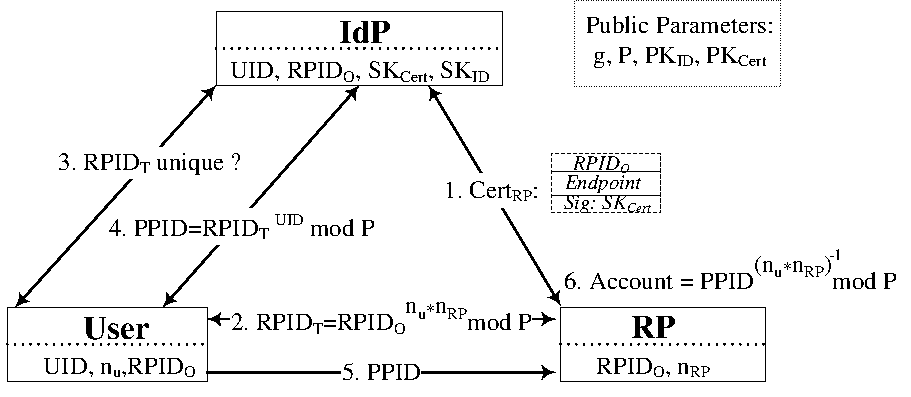
\includegraphics[width=\linewidth]{fig/Overview.pdf}
  \caption{Overview of Recluse.}
  \label{fig:overview}
\end{figure}
\end{comment}

\subsection{Goals}
As analyzed in Section~\ref{subsec:solutions}, to enhanced requirements of SSO systems, Recluse has to allow only the exact RP to derive the user's unchanged account with a trapdoor, bind the proof with a transformation of RP’s identifier, and achieve user-centric confidentiality of the identity proof. We further divide these three requirements into 5 goals and achieve these 5 goals using 5 phases which is formed as the process flow in Recluse:
\begin{itemize}
  \item 1. Providing a self-verifying value for the user-centric check (for \textbf{User-centric Confidentiality}), to ensure the correct construction and transmission of identity proof (i.e., user-centric confidentiality), which is achieved in RP initial registration (step a, b in Figure~\ref{fig:overview}), applying for a RP certificate ($Cert_{RP}$), a self-verifying value;
  \item 2. Providing a RP identifier transformation (for \textbf{Transformed Binding}), to ensure the security by binding the identity proof with this transformation, and preserve user's privacy by preventing the IdP from inferring the original RP identifier from this transformation in the request, achieved in RP identifier transforming (step 2.1 in Figure~\ref{fig:overview}) generating transformation (denoted as $PRPID$) of RP's original identifier (denoted as $RPID$);
  \item 3. Checking the uniqueness of the transformation (for \textbf{Transformed Binding}), to avoid one identity proof being accepted by two or more RPs, which will harm the security of SSO systems, achieved in Dynamic registration (step 2.2 in Figure~\ref{fig:overview}), checking the global uniqueness of $RPID$;
  \item 4. Unlinkable PID (for \textbf{Trapdoor-existing Identification}), for one user, the PIDs for different RPs should vary, to prevent identity linkage, which is achieved in $PID$ generation (step 4 in Figure~\ref{fig:overview}), generating PID at the IdP, and transferring PID to the RP; 
  \item 5. Unchanged account (for \textbf{Trapdoor-existing Identification}), to allow only the destination RP (with the trapdoor) to derive the unchanged account for one user from varying PIDs, which is necessary for providing the consecutive and individual services, achieved in $Account$ verifying (step 6 in Figure~\ref{fig:overview}), calculating the user's account in the RP.
\end{itemize}

\begin{comment}
As analyzed in Section~\ref{subsec:solutions}, to ensure the security and privacy of SSO systems, Recluse has to achieve user-centric confidentiality of the identity proof, bind the proof with a transformation of RP’s identifier, and allow only the exact RP to derive the user's unchange account with a trapdoor. We further divide these three solutions into 5 goals to be achieved in the design in Recluse:
\begin{itemize}
  \item 1. Providing a self-verifying value for the user-centric check, to ensure the correct construction and transmission of identity proof (i.e., user-centric confidentiality);
  \item 2. Providing a RP identifier transformation, to ensure the security by binding the identity proof with this transformation, and preserve user's privacy by preventing the IdP from inferring the original RP identifier from this transformation in the request;
  \item 3. Checking the uniqueness of the transformation, to avoid one identity proof being accepted by two or more RPs, which will harm the security of SSO systems;
  \item 4. Unlinkable PID, for one user, the PIDs for different RPs should vary, to prevent identity linkage. The $PID$ is generated at the IdP, and transferred to the RP.
  \item 5. Unchange account, to allow only the destination RP (with the trapdoor) to derive the unchanged account for one user from varying PIDs, which is necessary for providing the consecutive and individual services.
\end{itemize}

%To hide the user's traces from both the IdP and colluded RPs without breaking the security, Recluse has to achieve these : (1) the user and RP corporately calculate a transformation of the RP's identifier based on Discrete Logarithm Problem, which is sent to the IdP for binding with the identity proof while preventing the IdP from inferring the original RP identifier. The PIDs (in the identity proof) for a user in various RPs are different, to avoid the identity linkage. Moreover, only the RP (and the user) can calculate the trapdoor of the transformation, to transfer the PID into a unchanged account for the user.
\end{comment}

\begin{comment}
Recluse achieves these 5 goals using 5 phases as described in Figure~\ref{fig:overview}, while the used notations are listed in Table~\ref{tbl:notations}. The details are as follows, and the step refers to the one in Figure~\ref{fig:overview}:
\begin{itemize}
  \item RP initial registration: Applying for a RP certificate ($Cert_{RP}$), a self-verifying value,  (Step 1, Goal 1);
  \item RP identifier transforming: Generating transformation (denoted as $RPID_T$) of RP's original identifier (denoted as $RPID$), (Step 2, Goal 2);
  \item Dynamic registration: Checking the global uniqueness of $PRPID$, (Step 3, Goal 3);
  \item PID:  Generating PID at the IdP, and transferring PID to the RP, (Step 4 and 5, Goal 4);
  \item Account: Calculating the user's account in the RP, (Step 6, Goal 5).
\end{itemize}
\end{comment}

\begin{comment}
A RP certificate (denoted as $Cert_{RP}$) is the self-verifying value required in Goal 1, which is  generated in the \textbf{RP initial registration} (phase 1). A transformation (denoted as $PRPID$) of RP's original identifier (denoted as $RPID$) is generated in the \textbf{RP identifier transforming} (phase 2) for Goal 2. The global uniqueness of $PRPID$ is checked in the \textbf{dynamic registration} (phase 3) for Goal 3. The unlinkable \textbf{PID} is generated and transmitted to RP in the step 4 and 5 in Figure~\ref{fig:overview}, for Goal 4.

To achieve these goals, Recluse contains the following 6 phases, in which the IdP setup needs to be executed only once for a IdP, RP initial registration  needs to be invoked only once for a RP, while all the other phases will be invoked repeatedly for each user's login request at each RP. To make the decryption of Recluse clear, we list
\begin{itemize}
  \item IdP setup: Generating correct public parameters;
  \item RP initial registration: Applying RP certificate (denoted as $Cert_{RP}$) from IdP (Step 1 in Figure~\ref{fig:overview});
  \item RP identifier transforming: Generating transformation (denoted as $PRPID$) of RP's original identifier (denoted as $RPID$) (Step 2 in Figure~\ref{fig:overview});
  \item Dynamic registration: Checking the global uniqueness of $PRPID$ (Step 3 in Figure~\ref{fig:overview});
  \item PID:  Generating PID at the IdP, and transferring PID to the RP (Step 4 and 5 in in Figure~\ref{fig:overview});
  \item Account:  Calculating the user's account in the RP (Step 6 in Figure~\ref{fig:overview}).
\end{itemize}
\end{comment}

In Recluse, the IdP needs to be initialized during the IdP setup, for generating the public parameters for the users and RPs; the RP has to perform only one initial registration at the RP setup; and  the user triggers the Step 2-7 in Figure~\ref{fig:overview} for each login at a RP. IdP setup is performed at the very beginning of Recluse, and will be invoked by the IdP to update the leaked $SK_{Cert}$ or $SK_{ID}$, while $g$ and $P$ will never be modified. Recluse does not support multiple initial registrations for one RP, as the RP does not know the $UID$ nor the discrete logarithm of $RPID$ and fails to derive the user's new account  from the old one under the Discrete Logarithm problem.


\begin{table}[tb]
    \caption{The notations used in Recluse.}
    \centering
    \begin{tabular}{|c|c|}
    \hline
    {Notation} & {Definition} \\
    \hline
    {$P$} & {A large prime.} \\
    \hline
    {$g$} & {A primitive root  modulo $P$.} \\
    \hline
    {$Cert_{RP}$} & {A RP certificate.} \\
    \hline
    {$SK_{Cert}$, $PK_{Cert}$} & {The private / public key for $Cert_{RP}$.} \\
    \hline
    {$SK_{ID}$, $PK_{ID}$} & {The private / public key for  identity proof.} \\
    \hline
    {$UID$} & {User's unique identifier at IdP.} \\
    \hline
    {$PID$} & {User's privacy-preserving id in the identity proof.} \\
    \hline
    {$Account$} & {User's identifier at a RP.} \\
    \hline
    {$RPID$} & {RP's original identifier.} \\
    \hline
    {$PRPID$} & {The privacy-preserving $RPID$.} \\
    \hline
    {$n_u$} & {User-generated random nonce for $PRPID$. } \\
    \hline
    {$n_{RP}$} & {RP-generated random nonce for $PRPID$. } \\
    \hline
    {$Y_{RP}$} & {Public value for $n_{RP}$, $(RPID)^{n_{RP}} \ mod P$. } \\
    \hline
    {$t$} & {A trapdoor, $t=(n_u*n_{RP})^{-1} mod \ (P-1)$. } \\
    \hline
    \end{tabular}
    \label{tbl:notations}
\end{table}

\noindent\textbf{IdP setup.} In the setup, the IdP generates two random asymmetric key pairs, ($PK_{ID}$, $SK_{ID}$) and ($PK_{Cert}$, $SK_{Cert}$), for calculating the signatures in the identity proof and $Cert_{RP}$, respectively; and provides $PK_{ID}$ and $PK_{Cert}$ as the public parameters for the verification of identity proof and $Cert_{RP}$. Moreover, IdP generates a strong prime $P$, calculates  a primitive root ($g$) as described in Section~\ref{subsec:primitive}, and provides $P$ and $g$ as the public parameters. For $P$, we firstly randomly choose a large prime $Q$, and accept  $2Q+1$ as $P$ if $2Q+1$ is a prime. The strong prime $P$ makes it easier to choose $n_{u}$ and $n_{RP}$ as descried in Section~\ref{subsec:identifier-generation}. %With $g$, we obtain all the integers less than $P$, by calculating $g^i mod \ P$ for $0 \leq i \leq (P-1)$.

\subsection{RP Initial Registration}
\label{subsec:intialreg}
The RP invokes initial registration to apply a valid and self-verifying $Cert_{RP}$ from IdP (\textbf{Goal 1}) as provided in Figure~\ref{fig:registration}, which contains three steps:
\begin{itemize}
\item 1. RP sends IdP a $Cert_{RP}$ request $Req_{Cert_{RP}}$, which contains the distinguished name $Name_{RP}$ (e.g., DNS name) and the endpoint to receive the identity proof.
\item 2. IdP calculates $RPID = g^r mod \ P$ with a random chosen r which is coprime to $P-1$ and different from the ones for other RPs,  generates the signature ($Sig_{SK_{Cert}}$) of [$RPID, Name_{RP}$] using $SK_{Cert}$, and returns [$RPID, Name_{RP}, Sig_{SK_{Cert}}$] as $Cert_{RP}$.
\item 3. IdP sends $Cert_{RP}$ to the RP who verifies $Cert_{RP}$ using $PK_{Cert}$.
\end{itemize}

\begin{figure}
  \centering
  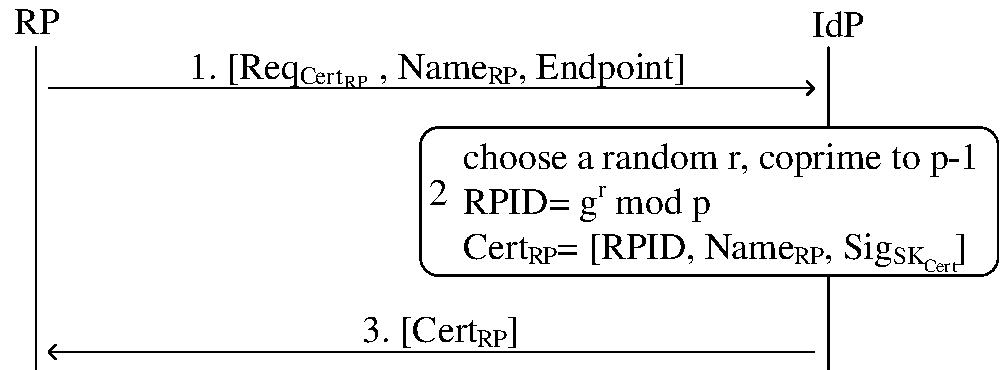
\includegraphics[width=\linewidth]{fig/registration.pdf}
  \caption{RP initial registration.}
  \label{fig:registration}
\end{figure}

%1. r which is coprime to $P-1$来保证$RPID$是一个本原根,从而保证adversary无法从PID中获取UID, ---
%2. $RPID$不能相同,保证RP无法进行identity linkage。 ---RP可以借助类似CT的方案来保证, 没有两个合法证书被颁发给同一个RPID
Here, we further explain the two requirements in the generation of $RPID$ for \textbf{Goal 4}:
\begin{itemize}
  \item $r$ should be coprime to $P-1$. This makes $RPID$ be another primitive root, and satisfies the requirement of Discrete Logarithm problem to prevent the RP  inferring $UID$ from $Account$.
  \item $r$ should be different with the ones for other RPs. Otherwise, the RPs who are assigned the same $RPID$, obtain the same PID for a user, which makes identity linkage possible.
\end{itemize}

The honest IdP is assumed to generate the correct $RPID$. However, we may perform an external check on $Cert_{RP}$ and $RPID$, based on the idea of Certificate transparency. The external check needs to be performed by a third party instead of RP who will be able to perform identity linkage with incorrect $RPID$. To perform the external check, IdP is required to provide the $Cert_{RP}$ to a log server, while a monitor checks the correctness of $Cert_{RP}$, i.e., no two valid $Cert_{RP}$ assigned to a same $RPID$ and $RPID$ is a primitive root modulo $P$ as descried in Section~\ref{subsec:primitive}. Moreover, $Cert_{RP}$ is compatible with a X.509 certificate which is discussed in Section~\ref{sec:discussion}.

\subsection{RP identifier transformation and Account calculation}
\label{subsec:identifier-generation}
In this section, we provide the calculation of $PRPID$, $PID$ and $Account$ separately, which is the foundation of each user's login process that described in Section~\ref{sebsec:loginprocess}.

{$PRPID$}. Similar to Diffie-Hellman key Exchange\cite{DiffieH76}, the RP and user generate the  $PRPID$ cooperatively as follows:
\begin{itemize}
  \item RP chooses a random odd number $n_{RP}$, and sends $Y_{RP} = {RPID}^{n_{RP}} mod \ P$ to the user.
  \item The user replies a random chosen odd number $n_{u}$ to the RP, and calculates $PRPID = {Y_{RP}}^{n_{u}} mod \ P$.
  \item RP also obtains $PRPID$ with the received $n_{u}$.
\end{itemize}

Therefore, $PRPID$ is denoted as Equation~\ref{equ:RPIDT}. The IdP fails to infer ${RPID}$ from $PRPID$ (\textbf{Privacy in Goal 2}).
   \begin{equation}
   PRPID = {Y_{RP}}^{n_{u}} = {RPID}^{n_{u}* n_{RP}} mod \ P
   \label{equ:RPIDT}
   \end{equation}

The generation ensures that $PRPID$ cannot be determined by neither (malicious) user nor RP, which prevents the adversary from constructing a identity proof to be accepted by two or more RPs (\textbf{Security in Goal 2}). RP fails to control the $PRPID$ generation, as it provides $Y_{RP}$ before obtaining $n_{u}$ and the modification of $Y_{RP}$ will trigger the user to generate another different  $n_{u}$. The Discrete Logarithm problem prevents the user from choosing a $n_{u}$ for a specified $PRPID$ on the received $Y_{RP}$.

Both $n_{RP}$ and $n_{u}$ are odd numbers, therefore $n_{RP}*n_{u}$ is an odd number and coprime to the even $P-1$, ensuring:
 \begin{itemize}
   \item $PRPID$ is a primite root modulo $P$, which prevents the RP from inferring $UID$ from $PID$ (\textbf{Goal 4}).
   \item The inverse $(n_{RP}*n_{u})^{-1}$ exists, that is, $(n_{RP}*n_{u})^{-1} * (n_{RP}*n_{u}) = 1 \ mod \ (P-1)$. The inverse  serves as  the trapdoor $t$ for $Accout$, which makes:
   \begin{equation}
   (PRPID)^t = RPID \ mod \ P
   \label{equ:trapdoor}
   \end{equation}
 \end{itemize}

{$PID$}. The IdP generates the $PID$ based on the user's $UID$ and the user-provided $PRPID$, as denoted in Equation~\ref{equ:PID}. $PID$ varies for RPs due to the uniqueness of $PRPID$, satisfying \textbf{Goal 4}.
 \begin{equation}
   PID = {PRPID}^{UID} \ mod \ P
   \label{equ:PID}
   \end{equation}

{$Account$}. The RP calculates $PID^t mod \ P$ as the  user's account, where $PID$ is received from the user and $t$ is derived in the generation of $PRPID$. Equation~\ref{equ:account} demonstrates that $Account$ is unchanged to the RP during a user's multiple logins, satisfying \textbf{Goal 5}.
 \begin{equation}
   Account = ({PRPID}^{UID})^t = {RPID}^{UID} mod \ P
   \label{equ:account}
   \end{equation}


\subsection{User Login Process}
\label{sebsec:loginprocess}
In this section, we present the detailed process for each user's login as shown in Figure~\ref{fig:process}. The process corresponds to the four phases defined in Section~\ref{subsec:overview}.

\begin{figure*}
  \centering
  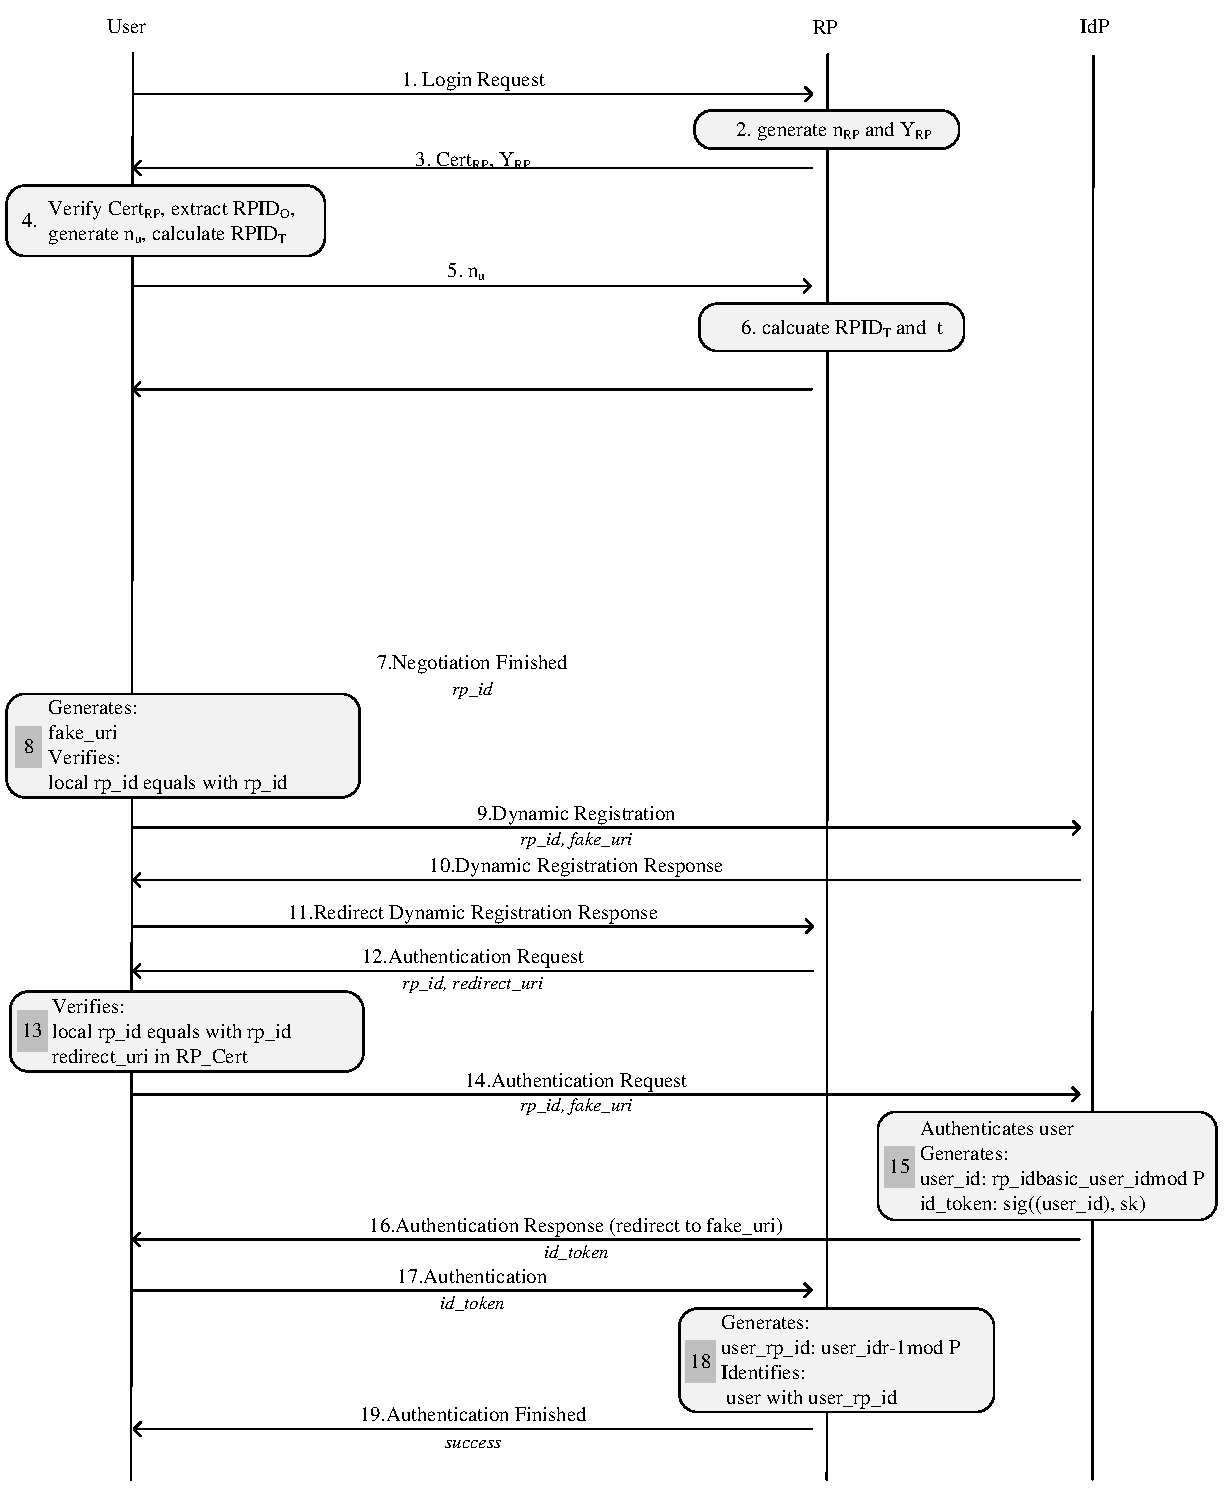
\includegraphics[width=\linewidth]{fig/process.pdf}
  \caption{Process for each user's login.}
  \label{fig:process}
\end{figure*}

For RP identifer transforming, the user and RP corporately process as follows. \textbf{(1)} The user sends a login request to trigger the negotiation of $PRPID$. \textbf{(2)} RP chooses the random $n_{RP}$, and calculates $Y_{RP}$ as described in Section~\ref{subsec:identifier-generation}. \textbf{(3)} RP sends $Cert_{RP}$ with $Y_{RP}$ to the user.  \textbf{(4)} The user halts the login process if the provided $Cert_{RP}$ is invalid; otherwise, it extracts $PID_O$ from $Cert_{RP}$, and calculates $PRPID$ with a random chosen $n_u$ as in Section~\ref{subsec:identifier-generation}. \textbf{(5)} The user sends $n_u$ and $PRPID$ to the RP. \textbf{(6)} RP calculates $PRPID$ using the received $n_u$ with $Y_{RP}$ as in Section~\ref{subsec:identifier-generation}, and rejects the user's login request if the calculated $PRPID$ is inconsistent with the received one. After that, RP derives the trapdoor $t$ as in Section~\ref{subsec:identifier-generation}, which will be used in calculating $Account$. \textbf{(7)} RP sends the calculated $PRPID$ to the user, who will halt the login if the received $PRPID$ is different from the cached one.

For dynamic registration, the user registers the RP at the IdP instead of RP as follows. \textbf{(8)} The user generates an one-time endpoint (used in Section~\ref{subsec:compatible}) if the received $PRPID$ is accepted. \textbf{(9)} Then, the user registers the RP with the $PRPID$ and one-time endpoint. \textbf{(10)} If $PRPID$ is globally unique and is a primitive root module $P$, IdP sets the flag $RegRes$ as $OK$ (otherwise $FAIL$), and constructs the reply in the form of 
[$RegRes$, $RegMes$, $Sig_{SK_{ID}}$] 
%[$RegRes$, $timestamp$, $PRPID$, $Sig_{SK_ID}$] where $timestamp$ is the time generating this reply and
where $RegMes$ is the response to traditional dynamic registration containing $PRPID$, issuing time with other attributes and $Sig_{SK_{ID}}$ is the signature of the other elements using the private key $SK_{ID}$ (satisfying \textbf{Goal 3}). \textbf{(11)} The user forwards the registering result to the RP. The user obtains $RegRes$ directly as the connection between the user and IdP is secure, while the RP accepts the $RegRes$ only when $Sig_{SK_{ID}}$ is valid
%, $timestamp$ is correct and $PRPID$ is the same as the cached one.
and $RegMes$ is issued for the $PRPID$ within the expiration date. The user and RP will negotiate a new $PRPID$ if $RegRes$ is $FAIL$.

To acquire the PID, the user corporates with the RP and IdP as follows. \textbf{(12)} RP constructs an identity proof request with the correctly registered $PRPID$ and the endpoint (the form of the request is detailed in Section~\ref{subsec:compatible}). \textbf{(13)} The user halts the login process if the received $PRPID$ is different from the previous one. \textbf{(14)} The user replaces the endpoint with the registered one-time endpoint, and sends it with the identity proof request to the IdP. \textbf{(15)} IdP requires the user to provide the correct credentials if the user hasn't been unauthenticated; and rejects the request if the binding of $PRPID$ and the one-time endpoint doesn't exist in the registered ones. Then, IdP generates the $PID$ as in Section~\ref{subsec:identifier-generation}, and constructs the identity proof with $PRPID$, $PID$, the valid period, issuing time and other attribute values, by attaching a signature of these elements using the private key $SK_{ID}$. \textbf{(16)} IdP sends the identity proof with the one-time endpoint to the user. \textbf{(17)} The user forwards the identity proof to the RP's endpoint corresponding to the one-time endpoint.

Finally, RP derives the user's unchanged $Account$ from $PID$ as follows. \textbf{(18)} RP accepts the identity proof only when the signature is correctly verified with $PK_{ID}$, $PRPID$ is the same as the negotiated one, the issuing time is less than current time, and the current time is in the validity period. If the identity proof is incorrect, RP returns login fail to the user who will trigger another login request. Otherwise, RP calculates the $Account$ as in Section~\ref{subsec:identifier-generation}. \textbf{(19)}, After obtaining the user's unchanged $Account$, RP sends the login result to the user and begins to provide the individual service.


\subsection{Compatible with OIDC}
\label{subsec:compatible}
Recluse is compatible with the implicit protocol flow of OIDC (authorization code flow is discussed in Section~\ref{sec:discussion}).

In Recluse, the formats of identity proof request and identity proof are the same as the ones in OIDC. In details, each element of the identity proof request in OIDC is contained in Recluse as follows: the RP's identifier ($PRPID$ in Recluse), the endpoint (one-time endpoint in the request from the user in Recluse) and the set of required attributes (also supported by Recluse although not listed in the description). The identity proof in Recluse is also exactly the same as the one in Recluse, which includes RP's identifer ($PID_T$ in Recluse), the user's PID, the issuer, validity period, issuing time, other requested attributes and a signature using the IdP's private key.

The same format of identity proof request and identity proof makes the verification same in OIDC and Recluse. The IdP, in both Recluse and OIDC, verifies the identity proof request, by checking whether the mapping of RP's identifier and endpoint exists in the registered ones. The RP, in both Recluse and OIDC, checks the correctness of identity proof, by checking that the signature is correct, the consistency of RP's identifer in the identity proof and the one it owns, the validity period, issuing time and the freshness (which is checked based on a nonce in  OIDC, while  $PRPID$ serves as the nonce in Recluse).

The RP's extra processes needed in Recluse may be achieved using the existing interfaces defined in OIDC.  Recluse requires that $PRPID$ is globally unique, which can be achieved through the dynamic registration (described in Section~\ref{sec:background}) provided by IdP in OIDC. In Recluse, the dynamic registration is invoked by the user instead of the RP to prevent the curious IdP infers the user's traces by analyzing the between the dynamic registration and identity proof request. To avoid the IdP to infer the RP's identity through the registration token in dynamic registration, the access control of the endpoint for dynamic registration is deleted in Recluse. As the registration response is transmitted through the user instead of server-to-server transmission between RP and IdP, the extra signature is required to guarantee the integrity of response. Moreover, the endpoint in the dynamic registration request is replaced with an one-time endpoint, to avoid the RP's identifying information to be leaked to the IdP.


The modification required by Recluse at the RP may be achieved using existing interface provided by the implementations of OIDC. Based on the software development kit (SDK) in existing OIDC implementations for RP, the Steps 2,3, 6, 12 (in Figure~\ref{fig:process}) in RP may be integrated in the interface for constructing identity proof request;
Step 18 in Figure~\ref{fig:process} may be combined with the interface for verifying and parsing identity proof.

The processes at the user may be achieved through an extension at the user agent, which captures the identity proof (and request) for process  without modifying existing message transmission at the IdP and RP (i.e., redirection mechanism), as described in Section~\ref{sec:implementation}.


Only the RP initial registration and Step 15 in Figure~\ref{fig:process} requires a modification at IdP.

\begin{comment}

The overview of login flow is shown in Figure~\ref{fig:overview}, which contains RP identifier negotiation, dynamic registration and token obtaining.

The of each phase in login flow is shown as follows:
\begin{itemize}
\item[1.] RP Identifier Negotiation: The negotiation is required to generate the RP identifier. For each SSO procedure, user is going to start negotiation with user. RP identifier is a random number which does not represent any RP, generated by rp-id-generating algorithm. However, the identifier is bound with specific authentication which is able to be confirmed by user and RP. The details of identifier generation is shown in Section~\ref{sec:identifier-generation}.
\item[2.] Dynamic Registration: Dynamic registration is required to in Recluse to make sure the identifier generated by negotiation is valid in IdP. In OIDC system, RP should register its attributes (e.g., the endpoint for identity proof) with IdP and obtain the RP identifier generated by IdP so that IdP is able to authenticate the user for specific RP. Therefore, to make sure the newly generated RP identifier in RP Identifier Negotiation is valid in IdP, the dynamic registration is required before the authentication request is transmitted to IdP. IdP is to check whether the identifier is unique and require RP to restart identifier negotiation if the identifier has be used by another RP.
%To make the RP identifier generated by negotiation is valid in IdP, user is to register this identifier with IdP through the dynamic registration API provided by IdP. IdP is going to check whether the identifier is unique and require RP to restart identifier negotiation if the identifier has be used by another RP.
\item[3.] Authentication: After dynamic registration, RP builds the authentication request and redirects it to IdP through user agent. After receiving the request, IdP firstly authenticates user and then issues identity proof for RP, which contains the user id generated through the user-id-generating algorithm. Then IdP redirects the identity to RP through user agent, and RP identify the user through identity proof. The methods of user identifier generation and RP identifying the user are shown in Section~\ref{sec:identifier-generation}.
\end{itemize}

However, in addition to the login flow in each authentication, the initial registration is required before the RP and user integrates the Recluse service. The initial registration allows the RP to achieve the necessary parameters from the IdP and user to sign on in the IdP. In Recluse system, the initial registration is conducted by each RP and user only once, however, the login flow is conducted in each authentication integrally each time.



\subsection{Initial Registration}
The initial registration between RP and IdP is shown as Figure~\ref{fig:registration}.
\begin{figure}
  \centering
  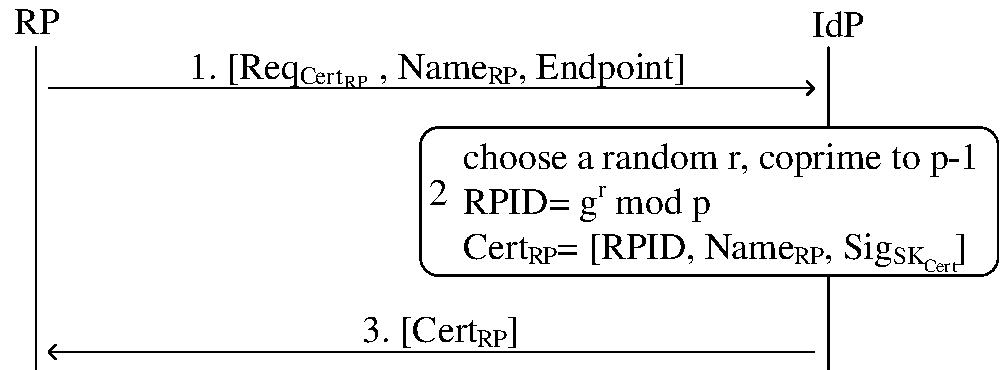
\includegraphics[width=\linewidth]{fig/registration.pdf}
  \caption{Prior Registration}
  \label{fig:registration}
\end{figure}
The registration process is as follows:
\begin{itemize}
\item[1.] Uploading Attributes: Firstly, IdP generates its prime $P$, the primitive root $g$ of $P$, used for RP and user identifier generation and the key pair $pk$, $sk$.
\item[2.]The RP uploads it attributes, such as its name, endpoint, identity proof (e.g., business license) and so on.
\item[3.] Issuing RP Certification: IdP verifies the identity of RP and generates the RP certification including $basic\_rp\_id$, $rp\_name$, \verb+redirect_uri+ and \verb+IdP_origin+.  The RP certification is used for user agent to verify the basic attributes, such as $basic\_rp\_id$ and \verb+redirect_uri+.
\item[4.]IdP returns the RP certification, $P$, $g$ and $pk$ to RP.
\end{itemize}

The initial registration required for IdP to verify the basic attributes of RP, such as name, endpoints for identity proof, so that Idp is able to provide the RP certification to RP which includes the unique identifier for each RP and its attributes. With the RP certification, user agent has the ability to verify the RP's endpoint for identity proof and notify user with RP's identity. Additionally, the parameters, prime $P$ (used for user id generating) with its primitive root $g$, public key of IdP $pk$ is provided in registration as well.
Same as RP, user need to register with IdP and IdP generates unique user id for each user.



\subsection{Rp-id-generating and User-id-generating algorithm}
\label{subsec:identifier-generation}
The rp-id-generating and user-id-generating algorithm are created based on Discrete Logarithm problem\cite{shiu2007cryptography:}.
IdP carefully chooses a big prime $P$\footnotetext[1]{$P$ is generated as $P=q\cdot 2+1$, while $q$ is prime as well.} and its primitive root \verb+g+ as generator for system. When the RP registers with IdP, IdP provides a unique primitive root as the RP's root identifier (called $basic_rp_id$).

For each login process, the user and RP negotiate the temporary RP identifier bound with specific authentication.
\subsubsection{$rp\_id$ generating}
While starting a login procedure, there is Diffie-Hellman key Exchange\cite{DiffieH76} between RP and user, through which the random $r$ is generated. However, to make sure that there is $r^{-1}$, that $r\cdot r^{-1}=1 mod \phi(P)$, $r$ should be the relative prime of $\phi(P)$, so that if $r$ is even $r$ should be added by one. Although there is little possibility that $r$ is the multiple of $p$ or $q$, it is not considered in the illustration. However, the re-negotiation is required in the practical system if $r$ is the multiple of $p$ or $q$. The RP identifier is generated as:
$$rp\_id=basic\_rp\_id^r mod P\eqno(1)$$
such that $rp_id$ is another primitive element module $p$. And $r^{-1}$ is generated through Extended Euclidean algorithm.
\subsubsection{$user\_id$ generating}
IdP labels each user at IdP with the unique identifier called $baisc\_user\_id$. To generate the specific user identifier for each $rp\_id$, the algorithm is
$$user\_id=rp\_id^{basic\_user\_id} mod P\eqno(2)$$
so
$$user\_id=basic\_rp\_id^{r\cdot basic\_user\_id}modP\eqno(3)$$
\subsubsection{Trapdoor}
While receiving $user\_id$ from IdP, RP is able to derive the constant user identifier from if
$$user\_rp\_id=user\_id^{r^{-1}} mod P\eqno(4)$$
so
$$user\_rp\_id=basic\_rp\_id^{(1 mod \phi(P))\cdot basic\_user\_id} mod P\eqno(5)$$
so
$$user\_rp\_id=basic\_rp\_id^{basic\_user\_id} mod P\eqno(6)$$
For single user in a RP, $user\_rp\_id$ is unchanged. However, $user\_rp\_id$s are distinct in each RP because $basic\_rp\_id$s are different in each RP.



\subsection{User Login Process}
\label{sebsec:loginprocess}
The login flow is shown as Figure~\ref{fig:process}, in which the $rp\_id$ is generated in step 6, the $user\_id$ is generated in step 15 and the RP derives the $user\_rp\_id$ in step 18.
\begin{figure*}
  \centering
  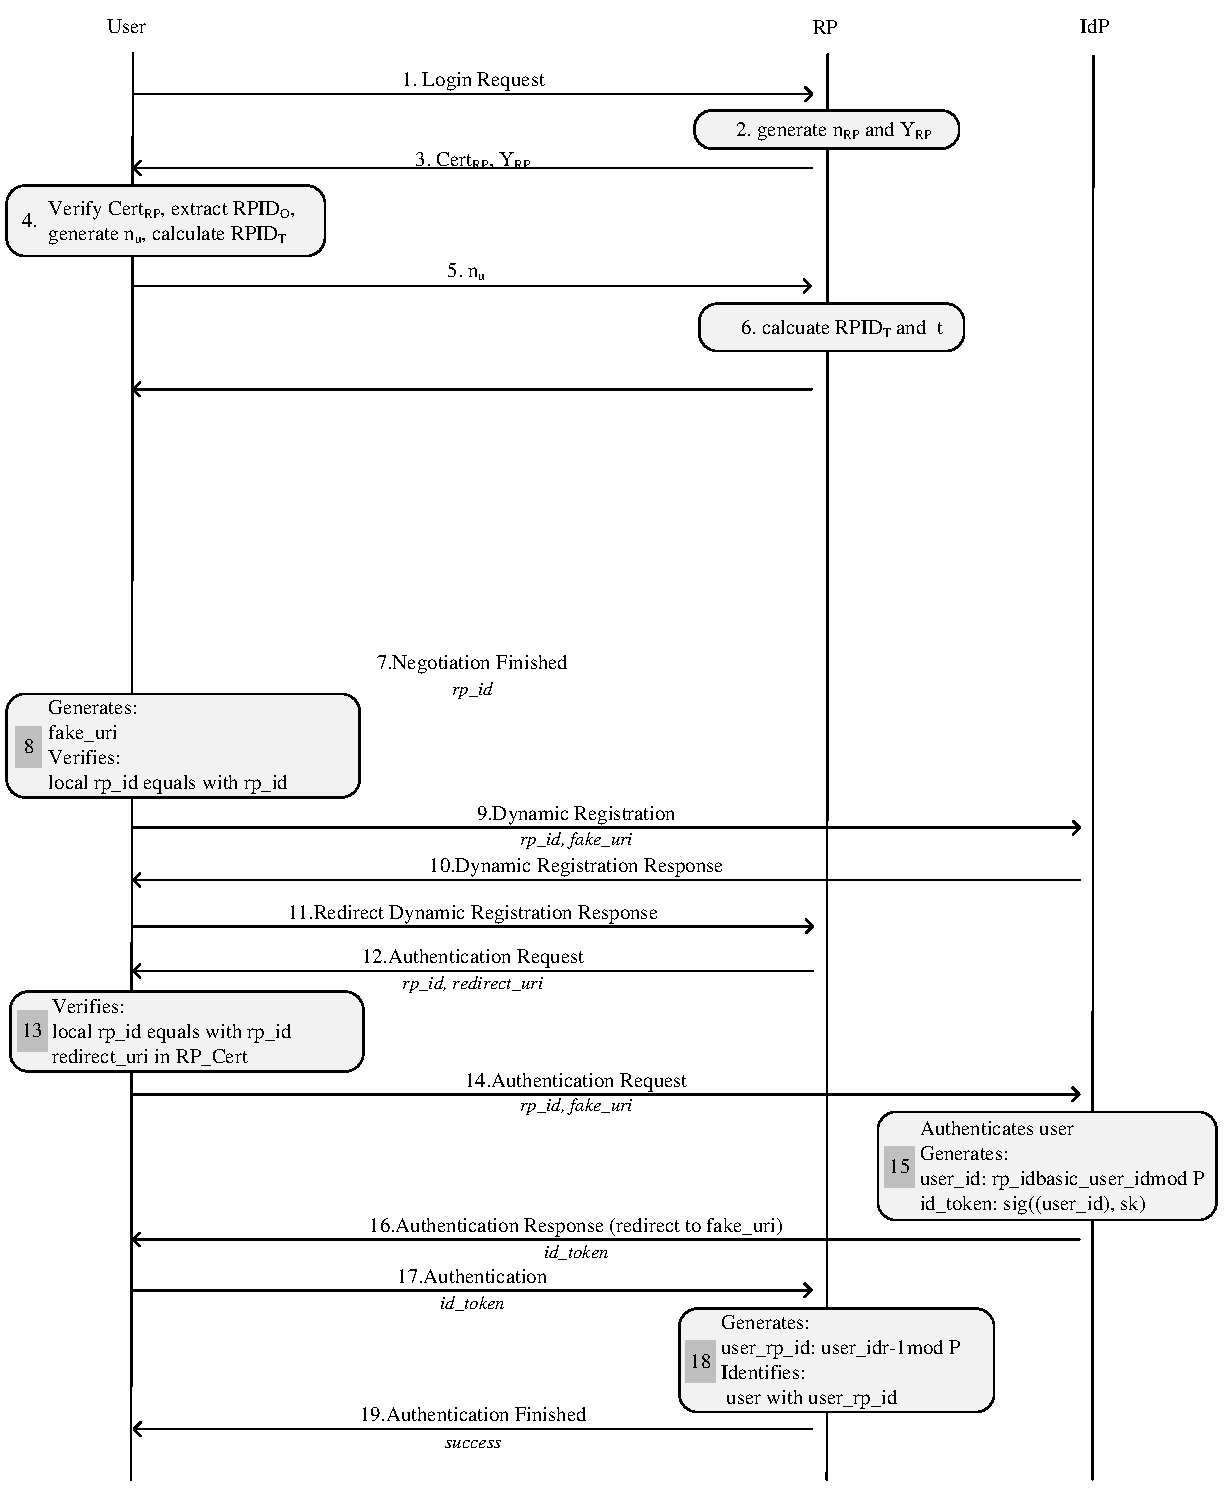
\includegraphics[width=\linewidth]{fig/process.pdf}
  \caption{Login Flow}
  \label{fig:process}
\end{figure*}

%抵抗phishing攻击:一定需要正确的RP参与,攻击者作为中间人
%1.使用IdP提供应用basic_rp_id与url的绑定,user agent保存映射
%缺点:占用空间,user agent需要缓存整个映射
%2.RP与用户通过加密的通道传输redirect_uri

%如果由RP选择basic_rp_id,那么多个rp之间的basic_rp_id有幂次关系,那么就可以关联用户

\subsubsection{RP Identifier Negotiation}
RP identifier negotiation starts form step 1 to step 7. The user accesses the service provided by RP in his/her browser. To log in this RP, user needs to click the login button offered by Recluse.
Firstly, the user agent sends the \verb+Start Negotiation+ request to RP, so that RP generates the random $sk\_rp$ and $pk\_rp=g^{sk\_rp}modP$ as the private key and public key for DH Key exchanging.
Secondly, RP builds the \verb+Negotiation Response+ with newly generated $pk\_rp$ as well as the \verb+RP_Cert+ issued by IdP. User agent similarly generates random $sk\_user$ and $pk\_user$, and $r=pk\_rp^{sk\_user}modP$. However, to make sure that $r$ is the relative prime of $\phi(P)$, it is required that $r$ should be odd and the greatest common divisor of $r$ and $\phi(P)$ is 1.
Then user agent continues the \verb+Negotiation+ sending $pk\_user$ and $r$ to RP. RP generates the local $r$ in the same way as user agent and compares the local $r$ and user agent generated $r$. If $r$s are equal, RP generates $rp\_id=basic\_rp\_id^rmodP$, as well as $r^{-1}$ through Extend Euclidean algorithm, which meets $r\cdot r^{-1}=1mod\phi(P)$.
Finally RP transmits the $rp\_id$ to user agent.
\subsubsection{Dynamic Registration}
Dynamic registration is from step 8 to step 13. While user agent receives teh $rp\_id$ from RP, it is required the $rp\_id$ from RP should be equal with it generated by user agent. Then user agent generates the \verb+fake_uri+ which contains the random string and keeps it for further identity proof transmission. User agent sends the \verb+Dynamic Registration+ request to IdP with newly generated $rp\_id$ and \verb+fake_uri+ and redirects the \verb+Dynamic Registration Response+ to RP.
\subsubsection{Authentication}
Authentication is from step 14 to step 19. After dynamic registration,  RP builds the \verb+Authentication Request+ including $rp\_id$ as well as the \verb+redirect_uri+ representing the endpoint, and redirects it to IdP through user agent. User agent tampers the authentication request, compares $rp\_id$ with the local one, verifies the validation of the \verb+redirect_uri+ and replaces it with the fake one. Then user agent transmits the \verb+Authentication Request+ to IdP. After receiving the request, IdP firstly authenticates user and then generates $user\_id=rp\_id^{basic\_user\_id}modP$. The identity proof signed with IdP's private key including the $user\_id$ is redirected to the \verb+fake_uri+ through user agent, who intercepts the transmission and transmit it to the endpoint \verb+redirect_uri+ in authentication request. Finally, RP derives the constant $user\_rp\_id$ from $user\_id$. If the $user\_rp\_id$ has already been registered, RP send \verb+Authentication Finished+ with the message \verb+success+ to user agent.

%描述user_id, rp_id and user_rp_id的生成
\end{comment}

\section{Security Analysis}
\label{sec:analysis}
%敌手目标:
%获得用户登录轨迹
%以受害者的身份登录RP
%使受害者以攻击者身份登录RP
%In SSO system, it is considered that an adversary tries to achieve the following goals:
%\begin{enumerate}
%    \item Privacy undermining attack: Malicious opponent tries to get user's login trace on different RPs.
%    \item Impersonation attack: Attacker tries to log in RP as a victim's identity. In this way, attacker can get the full control of victim's account in RP.
%    \item Abduction attack: Attacker also tries to lead user to upload users personal information to it. To achieve this goal, there are two ways. The first is letting a victim log in an RP as attacker's identity. In this way, if the RP is online storage system, victim may upload its privacy data to attacker's account. The other way is phishing attack. A malicious RP disguises it as another RP and abducts user to upload some information.
%\end{enumerate}
%
In order to prove the privacy and security properties of Recluse system, we firstly demonstrate that for any adversary in the system, a user's access to an specific  RP untraceable from it to another one. Besides, we illustrate the potential attacks discussed in the previous work about SSO security and the security issues introduced by Recluse.


\subsection{Privacy}
We now define the undistinguishability of SSO system. It is in the SSO system, for an adversary controlling curious IdP, it is impossible to inspect whether two \verb+authentication flow+s are to same RP or not, however, for an adversary controlling malicious RPs, it is impossible to inspect whether two \verb+authentication flow+s are from same user or not.

Assuming there are two \verb+authentication flow+s from the same user to the same RP. In Recluse system, for the curious IdP, the only parameter related with RP is $rp\_id$, as other parameters are related or generated by user, such as $fake\_uri$. To break the undistinguishability, IdP tries to derive the $basic\_rp\_id$ of RP from $rp\_id$ or inspect whether the $rp\_id$s are generated by the same $basic\_rp\_id$. However, as $rp\_id$ is generated by the formula (1), so
$$basic\_rp\_id=rp\_id^{r^{-1}}modP\eqno(7)$$
However, $r$ and $r^{-1}$ is unknown to the IdP, so that IdP is unable to derive the $basic\_rp\_id$ from the $rp\_id$. Moreover, even the IdP suspects that the $rp\_id$ is generated by the specific RP, it is impossible for IdP to verify it as the  $rp\_id$ can be generated based on any primitive root of $P$. Besides, assuming that the $rp\_id$s in different \verb+authentication flow+s are $rp\_id_1$ and $rp\_id_2$ generated by $r_1$ and $r_2$. There is
$$rp\_id_1=rp\_id_2^{r_1/r_2}modp\eqno(8)$$
So only the entity who carries the $r_1$ and $r_2$ is able to verify whether $rp\_id_1$ and $rp\_id_2$ generated by the same RP.

Inspecting whether the users in two \verb+authentication flow+s are the same user relies on the $baisc\_user\_id$ or the relation between $user\_id$s or $user\_rp\_ids$. Assuming the same user log in different RPs where the $user\_id$s are $user\_id_1$ and $user\_id_2$, $user\_rp\_id$s are $user\_rp\_id_1$ and $user\_rp\_id_2$, and $basic\_rp\_id$s are $basic\_rp\_id_1$ and $basic\_rp\_id_2$. We define that $\alpha=\log_{basic\_rp\_id_2}basic\_rp\_id_1$. There is
$$user\_rp\_id_1=user\_rp\_id_2^\alpha\eqno(9)$$
and
$$user\_id_1=user\_id_2^{\alpha\cdot r_1/r_2}\eqno(10)$$
The $\alpha$ is unknown to the malicious, so that the adversary is unable to  inspect whether the two \verb+authentication flow+s are from the same user. However, the malicious also tries to lead the same user in two \verb+authentication flow+s using the same $user\_rp\_id$ or $user\_id$. According to formula (2) and (4), the user should use the same $basic\_rp\_id$ or $rp\_id$ in two \verb+authentication flow+s. So the $user\_rp\_id$ is impossible to be same as $basic\_rp\_id$ is issued by IdP and verified by user agent. And $rp\_id$ is generated through the negotiation between user and RP, so that RP is unable to lead the user to use the same $rp\_id$ in different \verb+authentication flow+s.

\subsection{Security Consideration in OpenID Connect}
As it has been defined in ~\cite{OpenIDConnect} Section 16, the security consideration of the OIDC design contains authentication and authorization. Now we list the security consideration of authentication and prove that Recluse achieves this goals.
\begin{enumerate}
\item \textbf{Server Masquerading. } The malicious server might masquerade as the RP or IdP using various ways through which user might leak its identity proof for RP or credentials on IdP. The Recluse mitigate this threat in following ways. 1) The server visited through user agent is authenticated by HTTPS; 2) The user agent verifies the RP certification which makes sure that the token is only sent to the corresponding RP instead of the masqueraded one; 3) The user agent only visit the IdP's endpoint listed in the RP certification which avoid the access to the masqueraded IdP.
\item \textbf{Token Manufacture/Modification. } The adversary might generate a bogus token or tamper the contents in the existing token, which enables the adversary log in any RP as any honest user. The receiver of token must have the ability to verify whether the token is issued by IdP without any modification or not. The token used in Recluse is signed by IdP with its private key, so that the token is unable to be constructed or modified.
\item \textbf{Access/ID Token Disclosure. } The adversary might try to obtain an honest user's token to the honest RP through various ways, which enables the adversary log in this RP as the honest user. It is required the tokenisi never exposed to anyone except the corresponding user and RP.
\item \textbf{Access/ID Token Redirect. } The malicious RP might use the token from an honest user to access other RPs as this user only if the token is also valid in other RPs. It is required the token issued for specific RP should bound with this RP which means the RP has the ability to verify whether a token is valid in itself. The token used in Recluse containing the $rp\_id$ and $user\_id$ is solely bound with specific RP and user, which is checked by the RP.
\item \textbf{Issuer Identifier. } The issuer identifier contained in the token should be completely same as it provided by the IdP, so that the verifier of token has the ability to obtain the corresponding public key. It is also implemented in Recluse.
\item \textbf{TLS Requirements. } To avoid network attacker the transmission in OIDC system should be protected by TLS. It is implemented in Recluse.
\item \textbf{Implicit Flow Threats. } In OIDC implicit flow, token is transmitted through user agent and the TLS protections are only between user agent and IdP, and between user agent and RP. It is required the token should not be leaked to the adversary by the user agent. The user agent of Recluse is deployed based on the Chrome browser as the trust base.
\end{enumerate}

It is discovered that the security consideration of authentication in OIDC can be included into the security consideration in Section~\ref{sec:background} as table ~\ref{tab:security-consideration}. however, the threats introduced by Recluse which breaks the security consideration and the methods to mitigate these threats has also been discussed in Section~\ref{sec:overview}.


\begin{table}\label{tab:security-consideration}
\caption{Security Consideration}
\begin{tabular}{|c|c|}
\hline  % 在表格最上方绘制横线
Security Consideration of SSO & Security Consideration of OIDC\\
\hline  %在第一行和第二行之间绘制横线
Content Checking& \multicolumn{1}{p{120pt}|}{Server Masquerading}\\
\hline
Confidentiality& \multicolumn{1}{p{120pt}|}{Server Masquerading, Access/ID Token Disclosure, TLS Requirements, Implicit Flow Threats}\\
\hline
Integrity& \multicolumn{1}{p{120pt}|}{Token Manufacture/Modification, Issuer Identifier}\\
\hline
Binding& \multicolumn{1}{p{120pt}|}{Access/ID Token Redirect}\\
\hline
\end{tabular}
\end{table}

\subsection{Related Security Analysis}
\noindent\textbf{307 Redirect. }It has been discussed in~\cite{FettKS16} that IdP might redirect the user to the RP immediately after the user inputs the credentials. For example, the HTTP response to the user's POST message with \verb+username+ and \verb+password+ might be the redirection to RP carrying user's identity proof. That is, as long as the 307 status code is used for this redirection, the user's credentials are also transmitted to the RP. However, in Recluse the redirections are intercepted by the user agent and rebuild the HTTP GET request to RP or IdP which is unable to leak the POST data of the user.

\noindent\textbf{IdP Mix-Up. } It has been illustrated in~\cite{FettKS16} that the adversary might intercept the the user's access to RP and modify the user's choice of IdP, assuming that RP integrates the SSO service provided by both the honest IdP (named \verb+HIdP+) and malicious IdP (named \verb+MIdP+). The user obtains the \verb+access token+ and \verb+authorization code+ from the \verb+HIdP+ and uploads them to the RP, however, the RP considers that the \verb+access token+ and \verb+authorization code+ are issued by the \verb+MIdP+. Therefore, the RP tries to exchange for the protected resources using the \verb+access token+ and \verb+authorization code+ with \verb+MIdP+. With this, the adversary carries the honest user's \verb+access token+ and \verb+authorization code+ which make the adversary able to log in this RP as the identity of the honest user. However, the threat is mitigated by the OIDC implicit flow, as the \verb+ID token+ issued by IdP contains the issuer identifier, so that RP is able to find out which IdP the token is from.

\noindent\textbf{Cross-Site Request Forgery (CSRF). } The CSRF attack on the RP makes the identity injection possible, through which the adversary might lead the honest user to upload the adversary's \verb+ID token+ to the RP. However, in Recluse the cross origin request should be repudiated by both RP and IdP excepted the request from the origin of the user agent. Therefore the CSRF attack on Recluse is impossible.


\begin{comment}
PRIOIDC tries to protect user's privacy by keeping RP anonymous to IdP. IdP is able to get client\_id and redirect\_uri. As redirect\_uri is generated by user, it will show nothing about RP. IdP can only undermine user's privacy by get RP's identity from client\_id. It's described in Client-id-generating algorithm: $client\_id=basic\_rp\_id^r mod p$. $p$ is a large prime and basic\_rp\_id is a primitive element module $p$. And $r$ is the random number generated by user and RP. IdP can only find out RP's real identity by finding out $r^{-1}$ and let $1=r\cdot r^{-1} mod (p-1)$, so that $$basic\_rp\_id=client\_id^{r^{-1}}modp$$
But $r$ is secret shared by user and RP, and according to \textbf{Discrete Logarithm} problem calculating $r$ from client\_id is difficult. So basic\_rp\_id is invisible to IdP. In other way if IdP gets a user's repeatedly login, it is going to find out whether they are about the same RP. If there are two client\_ids from the same RP marked as $client\_id_{1}=basic\_rp\_id^{r_1}modp$ and $client\_id_{2}=basic\_rp\_id^{r_2}modp$. Client\_id$_{1}$ and client\_id$_{2}$ meet the following formula
$$client\_id_1=client\_id_2^{r_2/r_1}modp$$
So that only when knowing $r_1$ and $r_2$ IdP can find out the relevance between Client\_id$_{1}$ and client\_id$_{2}$. But $r_1$ and $r_2$ are invisible to IdP. So IdP is never able to undermine user's privacy.

RPs try to find out user's login trace in three ways: 1) Getting the user's unique id in IdP. 2) Finding the relevance among user\_rp\_ids. 3) Deducing user's login trace from IP address. As user's id is used in generating user\_id in id\_token, RP is able to obtain $user\_id=client\_id^{id}modp$. Client\_id is primitive element module $p$. Although client\_id, user\_id and $p$ are known by RP, according to \textbf{Discrete Logarithm} problem calculating id from user\_id is difficult. For different RPs, they are able to get user's user\_rp\_id. User\_rp\_ids from different RPs can be marked as $user\_rp\_id_1=basic\_rp\_id_1^{id}modp$ and $user\_rp\_id_2=basic\_rp\_id_2^{id}modp$. As basic\_rp\_id$_1$ and basic\_rp\_id$_2$ are primitive element module $p$, there is $0<\alpha<p$ and $basic\_rp\_id_1=basic\_rp\_id_2^\alpha modp$.So user\_rp\_id$_1$ and user\_rp\_id$_2$ meet the following formula
$$user\_rp\_id_1=user\_rp\_id_2^\alpha modp$$
So RP is able to deduce the relevance between user\_rp\_id$_1$ and user\_rp\_id$_2$ only when knowing $\alpha$. As basic\_rp\_id is generated by IdP and calculating $\alpha$ from basic\_rp\_ids, RP is never able to find the relevance. If an RP does not use the basic\_rp\_id from IdP, user is able to find it dishonest through rp\_certificate and stop the login. Most of current users use dynamic IPs so that it is impossible to get user's login trace from user's IP.


\subsection{Impersonation attack}
RP conducts impersonation attack by getting user's id\_token which is valid in other RPs. OpenID Connect protocol protect id\_token from malicious RP by keep RP owns unique client\_id and check RP's redirect\_uri during login. Unique client\_id makes one RP's id\_token invalid in other RPs. And IdP only redirects id\_token to it's relevant RP's redirect\_uri registered in IdP so that attacker is never able get RP's id\_token. There are three conditions for a malicious to try getting a validate id\_token. 1) Malicious RP has already finished client\_id negotiation with an RP as a user. As client\_id is generated by both RP and user, malicious RP is unable to get the id\_token with the same client\_id. 2)Malicious RP has got a user's id\_token, same as condition 1 malicious RP is unable to negotiate the same client\_id with another RP. 3) Malicious RP acts as the man in the middle between RP and user. As RP sends its URL in rp\_certificate user only sends its id\_token to this URL so that attacker can never achieve id\_token. As a summary, malicious is unable to conduct impersonation attack.

Malicious user is only able to conduct impersonation attack by tempering id\_token. If attacker has already get victim's user\_rp\_id, attacker is able to calculate $user\_id=user\_rp\_id^rmodp$. $r$ is shared by RP and attacker. However id\_token is protected by the signature generated by IdP so that it is impossible for attacker to log in RP as victim.

%External attacker is going to steal user's id\_token from network flow to make the attack. As all the network flows are protected by https, external attacker is unable to conduct the attack.
\subsection{Abduction attack}
To lead user to login an RP as attacker, attacker needs to make sure that user receive a malicious token from IdP. As https is used to protect parameters transforming between user and IdP, it's impossible to temper user's token during transmission. The other way to conduct the attack is phishing attack on IdP.
In traditional SSO protocol such as OAuth 2.0 and OpenID Connect, it is possible for malicious to conduct phishing attack on IdP. As it is shown in ~\ref{fig:OpenID} step 2, the request from user to IdP is built by RP. If an malicious RP set the IdP'url as its phishing site, an unwary user may input its id and password on the phishing website so that attacker is able to get the full control of user's account.
In PriOIDC as RP\_Cert contains IdP's url, user agent is going to compare the IdP's url in request and RP\_Cert. If they are not matched, the request is deemed invalid.

Phishing attack on RP in SSO system is quite different from it in normal website. In SSO system even an unwary user has visited a phishing RP's website, IdP is going to ask user to make sure RP's identity in ~\ref{fig:OpenID} step 2. The identity is bound with RP's client id and client id is bound with its redirect uri. If malicious RP constructs the request in ~\ref{fig:OpenID} step 2 to IdP with its personal client id, user is able to find out the true identity of RP and protect itself from phishing attack. In traditional SSO system if malicious uses a client id of another RP, IdP is going to redirect user to the corresponding redirect uri. In PriOIDC user agent is going to compare redirect uri from RP with the redirect uri in RP\_Cert.If uris are not matched, the request is regarded invalid. A phishing RP can never achieve another RP's token and never lead user to log in its website.

%In phishing attack, adversary forges an RP's web application and induces user to log in it. In the disguise of the real RP, phishing site must send the real RP's rp\_token to user. In obtaining token phase if RP redirects user to real IdP, user is going to send its id\_token to the address from rp\_certificate. RP is not able to get user's id\_token and User does not log in adversary's RP finally. If RP redirects user to a fake IdP, the URL in redirection request is not mapped with it in rp\_certificate. User is going to stop the login. So phishing attack is not possible.

%External attacker is willing to conduct abduction attack. Attacker is going to make the attack by temper user's id\_token into attacker's id\_token when id\_token is transformed on the network. But all the network flows are protected by https so that user's id\_token is secure.
%如果不同RP之间Basic_Client_ID 找到幂次的关系,那么就可以对应到同一个用户的身份


\subsection{Discussion}
An external attacker is also taken into account in SSO system. External attacker is able to capture and temper all the network flow through user, RP and IdP. External attacker's targets include impersonation attack, abduction attack and privacy undermining attack.
%As SSO login requires IdP and RP to adopt https, external attacker is unable to get user's login trace through network flows. And user's dynamic IP makes external attacker impossible to get user's login trace from user's IP.
If an attacker keeps its eye on a specific user, it is able to find that the user's login on different RPs. So it is easy for an external attacker to draw a user's login trace. Privacy protection is not effective for external attacker.
To protect user from privacy leaking a proxy is probably a appropriate scheme. Proxy is able to mix multi-user's request and keep user's login trace invisible to attacker. User's dynamic IP makes proxy impossible to get user's login trace from user's IP
External attacker is going to steal user's id\_token from network flow to make the attack and it is also going to make the attack by temper user's id\_token into attacker's id\_token when id\_token is transformed on the network. As all the network flows are protected by https, external attacker is unable to conduct the attacks.
\end{comment}

\section{Implementation}
\subsection{Evaluation}
\label{sec:evaluation}
We have compared the processing time of each user login in Recluse, with the original OIDC implementation (MITREid Connect) and SPRESSO which only hides the user's accessed RPs from IdP.

%(with 4 cores, 8 threads)\
\noindent{\textbf{Environment.}} We run the evaluation on 3 physical machines connected in a separated 1Gbps network. A DELL OptiPlex 9020 PC (Intel Core i7-4770 CPU, 3.4GHz, 500GB SSD and 8GB RAM) with Window 10 prox64 works as the IdP. A ThinkCentre M9350z-D109 PC (Intel Core i7-4770s CPU, 3.1GHz, 128GB SSD and 8GB RAM) with  Window 10 prox64 servers as RP. The user adopts Chrome v75.0.3770.100 as the user agent on the Acer VN7-591G-51SS Laptop (Intel Core i5-4210H CPU, 2.9GHz, 128GB SSD and 8GB RAM) with  Windows 10 pro. For SPRESSO, the extra trusted entity FWD is deployed on the same machine as IdP. The monitor demonstrates that  the calculation and network processing of the IdP does not become a bottleneck. For SPRESSO, one extra stronger host is adopted to deploy the user agent for better performance as analyzed later.

\noindent{\textbf{Performance.}} We have measured the processing time for $1000$ login flows, the the results is demonstrated in Figure~\ref{fig:evaluation}. The average time is 208 ms, 113 ms and 308 ms for Recluse, MITREid Connect and SPRESSO respectively. Compared to the original OIDC implementation (i.e., MITREid Connect), Recluse requires about the extra 95 ms processing time, which is composed of RP identifier transforming (about 46 ms), dynamic registration (about 52 ms), $PID$ generation (6 ms), and $Acount$ calculation (about 44 ms), but reduces in identity proof transmission (about 43 ms) and minus the of authentication request initiation (about 10 ms). In details, the time for calculating $t$ through Extended Euclidean algorithm needs about 3 ms; the processing time of modular exponentiation, required in the calculation of $PRPID$, and $PID$, varies in the user (about 22 ms), IdP (about 2 ms) and RP (about 3 ms), as the execution of  JavaScript implementation (at the user) requires more time than the Java implementations (at IdP and RP). Moreover, the modular exponentiation in $Account$ requires about 46 ms, as the discrete logarithm $t$ is no longer than 2048 bits, much longer than the $n_{RP}$ and $n_{u}$ (not longer than 256 bits) for $PRPID$.

For better comparison, we further divide a SSO login flow into 4 phases, which : 1. \textbf{authentication request initiation (step 1-14 in Figure~\ref{fig:process})}, the period which starts before the user sends the login request and ends after the user receive the identity proof request transmitted from itself. 
%IdP has received the identity proof request; 
2. \textbf{identity proof generation (step 15 in Figure~\ref{fig:process})}, denoting the construction of identity proof at the IdP (excluding the user authentication); 3. \textbf{identity proof transmitting (step 16-17 in Figure~\ref{fig:process})}, for transmitting the proof from the IdP to the RP with the user's help; and 4. \textbf{identity proof verification (step 18 in Figure~\ref{fig:process})}, for the RP  verifying and parsing the proof for the user's $Account$. However, the http transmission is consisted of the pairwise request and response, so that in the implementation of timer, the step 14 and 19 are counted as the identity proof transmitting. To avoid the time difference in each computer, we consistently anchor the time point at user agent where the time is always achieved from the user's PC. The detailed comparison is shown in Figure~\ref{fig:evaluation}.



\begin{figure}
  \centering
  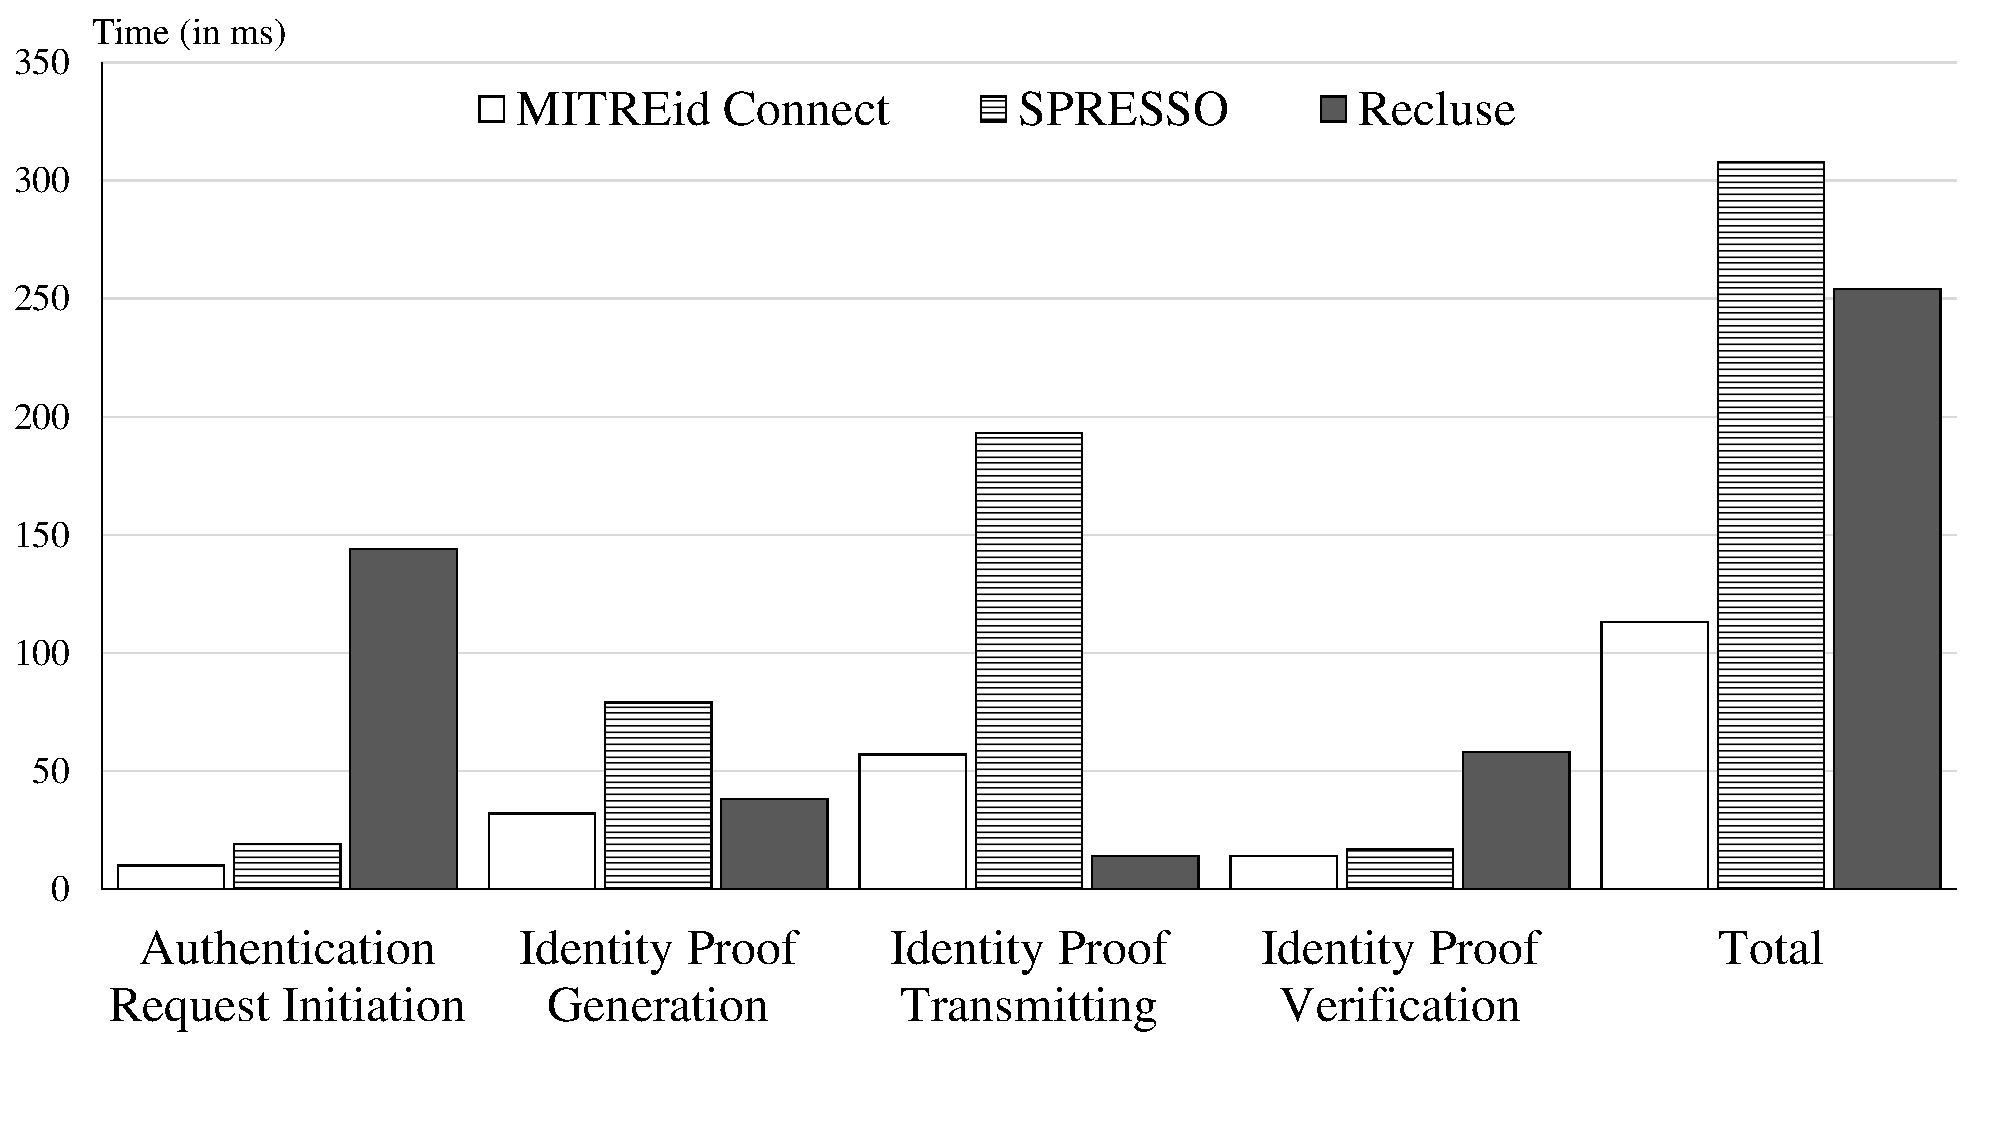
\includegraphics[width=\linewidth]{fig/evaluation2.pdf}
  %\subfigure[Authorization Code Flow]{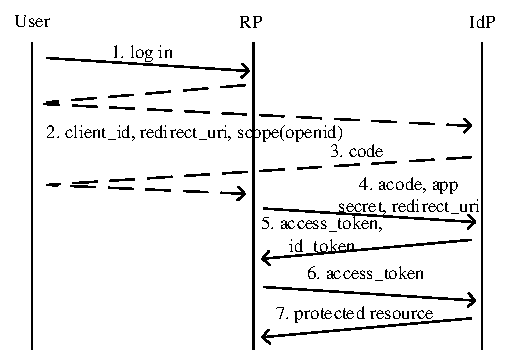
\includegraphics[width=\linewidth]{fig/openidconnect2.pdf}\label{fig:OpenID_code}}
  %\subfigure[Hybrid Flow]{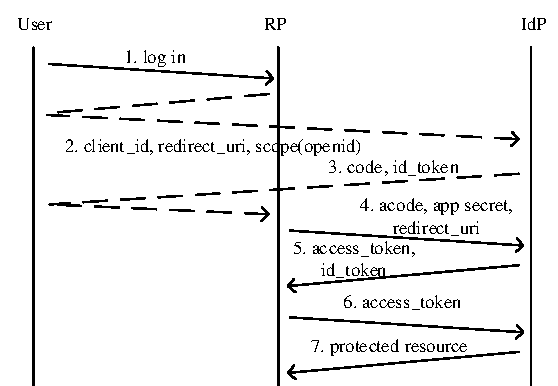
\includegraphics[width=\linewidth]{fig/openidconnect3.pdf}\label{fig:OpenID_hybrid}}
  \caption{The Evaluation.}
  \label{fig:evaluation}
\end{figure}
In the authentication request initiation, MITREid Connect requires the shortest time (10 ms); SPRESSO needs 19 ms for RP to obtain the IdP's public information and encrypt its domain; Recluse needs 98 ms, for the $PRPID$ calculation (1 modular exponentiation at the user and 2 at the RP) and dynamic registration.

For identity proof generation, MITREid Connect needs 32 ms (information constructing and signing); Recluse needs an extra 6 ms for the generation of $PPID$;  SPRESSO requires 71 ms for a different format of identity proof, which is longer that the other two as the processing in SPRESSO is implemented with JavaScript while the others are using Java.

For identity proof transmitting, IdP in  MITREid Connect provides the proof as a fragment component (i.e., proof is preceded by \#) to RP to avoid the reload of RP document; and RP uses the JavaScript code to send the proof to the background server; the total transmitting requires 57 ms. In Recluse, a chrome extension relays the identity proof from the IdP to RP, which needs 14 ms. The transmitting in SPRESSO is much complicated: The user's browser creates an iframe of the trusted entity (FWD), downloads the JavaScript from FWD, who obtains the RP's correct URL through a systematic decryption and communicates with the parent opener (also RP's document, but avoiding leaking RP to IdP) and RP's document through 3 post messages. 
%The time for transmitting identity proof in SPRESSO, relies on the performance of the user's host, 193 ms in our original user, and 127 ms in a stronger user.

In identity proof verification, the RP in MITREid Connect needs 14 ms for verifying the signature, SPRESSO requires 17 ms for a systematic decryption and signature verification, while Recluse needs 58 ms for calculation of $Account$ and signature verification.

\begin{comment}
The consideration of usability about Recluse is time cost in each authentication. However, the Recluse also introduces the extra storage as IdP and RP has to remember the longer identifier of user and RP. But the storage cost is within the range of TBs, which is to be ignored.

\subsection{Settings}
The prototype of Recluse has been implementation on the system consisting of 3 computers.
The IdP is on the DELL OptiPlex 9020 PC with an Intel Core i7-4770 CPU, 500GB SSD and 8GB of RAM running Window 10 pro. The RP is on the ThinkCentre M9350z-D109 PC with an Intel Core i7-4770s CPU, 128GB SSD and 8GB of RAM running Window 10 pro. The user agent is on the Acer VN7-591G-51SS Laptop with an Intel Core i5-4210H CPU, 128GB SSD and 8GB of RAM running Windows 10 pro.
The system is linked through the D-Link DGS-1008D Unmanaged Gigabit Ethernet Switch.

Additionally, the version of Chrome is 75.0.3770.100, and the version of Spring framework is 2.0.5.

The timer starts when the user click the login button and stops while the RP identifies the user. To run the login process automatically, the JavaScript code is inserted to the RP's web page to simulate the clicking the login button.

\subsection{Result}
We run the authentication on Recluse prototype system 1000 times and get the average time of the whole authentication flow is 208 ms. Compared with the traditional OIDC system, Recluse introduces the RP identifier transforming and dynamic registration, the average time cost of which are 46 ms and 52 ms. Additionally, Recluse also change the the generation of $PRPID$ and $PID$, which introduces extra Modular Exponentiation and Extended Euclidean computation. It is inspected that the Modular Exponentiation computation in $PRPID$ generating conducted by RP and user agent cost 3 ms and 22 ms, the computation conducted by IdP while generating $PID$ costs 2 ms, as the power in the above computations are not longer than 256 bits. While RP identifies the user, the trapdoor $t$ is generated by the Extended Euclidean algorithm, which costs 3 ms in average. Then RP derives the $Account$ from $PID$ by the Modular Exponentiation computation the power of which is $t$ no longer than 2048 bits, costing 46 ms in average.
%, in which the Negotiation costs 309 ms , the Dynamic Registration costs 129 ms, and the Authentication costs 107 ms.

%The most time cost is introduced by the modular power and extended euclidean operation. It is evaluated that the time cost of each modular power operation in RP, user agent and IdP are about 30 ms, 100 ms and 30 ms. During the login flow contains modular power operation is conducted 4 times by RP, 3 times by user agent and 1 time by IdP.


\subsection{Comparison}
We also run the unmodified MITREid Connect and SPRESSO (with the open-source project) system with the similar timer and automated scripts to see the comparison.
It is inspected that the time cost of MITREid Connect and SPRESSO are 69 ms and 295 ms at best. To compare Recluse with MITREid Connect and SPRESSO in detail, we formally split the authentication process in the SSO systems into specific phases,
\begin{itemize}
    \item  Authentication request initiated, which starts when the user agent sends the login request to RP and ends while IdP receives the authentication request.
    \item  Identify proof generated, the phase IdP generates the identity proof after receiving the authentication request.
    \item  Identity proof transmitted, from IdP sending the identity proof to RP receiving the Identity proof.
    \item  Identity proof verified, the phase RP identifies the user through the identity proof.
\end{itemize}

\begin{figure}
  \centering
  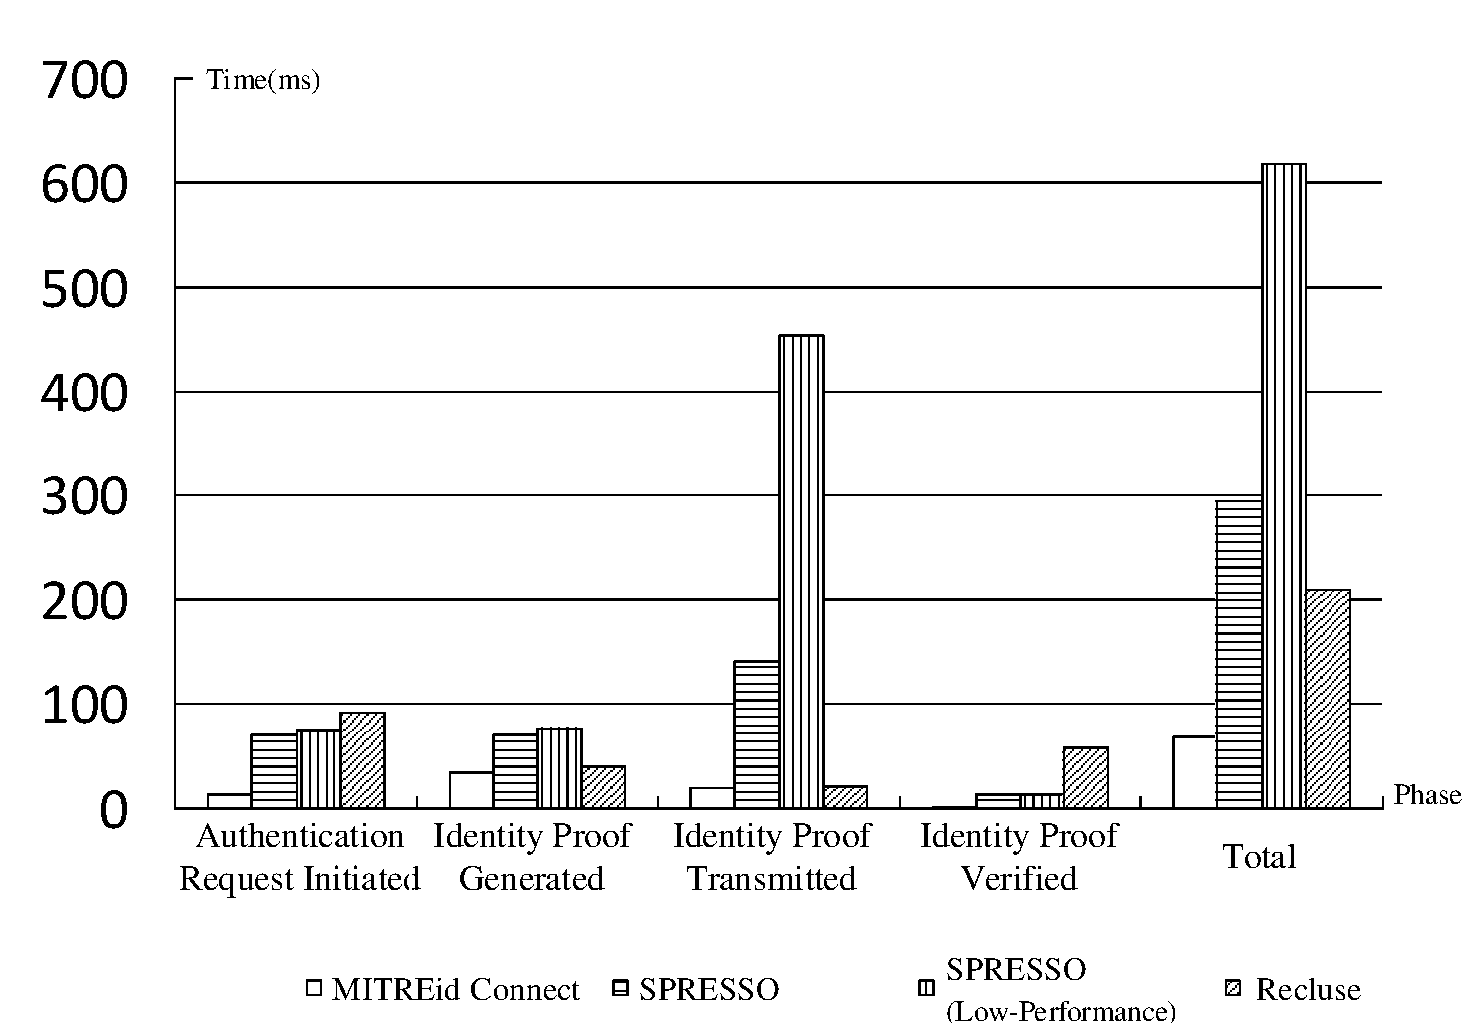
\includegraphics[width=\linewidth]{fig/evaluation.pdf}
  %\subfigure[Authorization Code Flow]{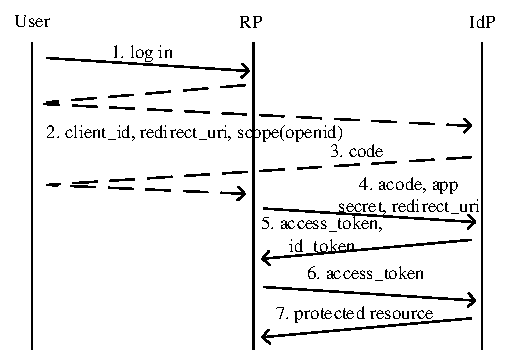
\includegraphics[width=\linewidth]{fig/openidconnect2.pdf}\label{fig:OpenID_code}}
  %\subfigure[Hybrid Flow]{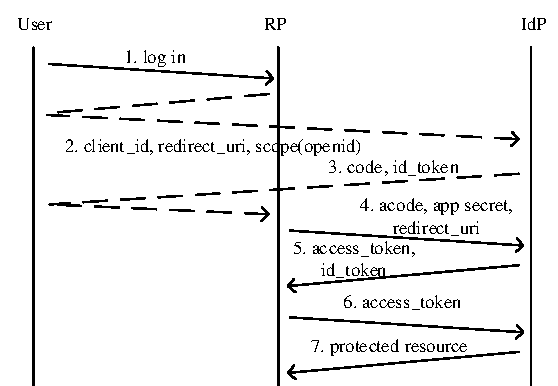
\includegraphics[width=\linewidth]{fig/openidconnect3.pdf}\label{fig:OpenID_hybrid}}
  \caption{The Evaluation.}
  \label{fig:evaluation}
\end{figure}
The comparison of Recluse, MITREid Connect and SPRESSO is shown as Figure~\ref{fig:evaluation}.

In the authentication request initiated phase, MITREid Connect uses the shortest time, 10 ms, as it only builds the request with the stored parameters, such as RP identifier and endpoint. SPRESSO introduces the additional request from RP to IdP for IdP's public parameters and the encryption operation to generate \verb+tag+ (the encrypted RP identifier), so that the time cost is 19 ms. Recluse use the longest time, 98 ms , which introduces the extra negotiation and dynamic registration in this phase including 1 time Modular Exponentiation computations at user agent and 2 Modular Exponentiation computations at RP.

In the phase of identity proof generated, all of the systems offer the signed identity proof. Compared with MITREid Connect, Recluse only introduces the extra Modular Exponentiation computation for $PPID$. However, the SPRESSO provides the totally different format of identity proof. The time cost in this phase of MITREid Connect, SPRESSO and Recluse are 32 ms, 78 ms and 38 ms.

In the phase of identity proof transmitted, Recluse transmits the identity proof through the extension and the MITREid Connect uses JavaScript code in RP's web page , the time cost of which are 14 ms and 57 ms. The SPRESSO requires the additional opened iframe, which downloads the script from FWD for extra encryption and decryption operation for identity proof transmitted. However, the time cost of these operations are significant different while running user agent in different devices. We get the 127 ms in average at best, however, in another low-performance device (), the number is 453 ms. To verify whether the performance of user agent has the same influence on Recluse, we use several PCs to log in Recluse and record the time. The result is the time costs in these PCs are quite similar which means the performance of user agent is not apparently influential with Recluse.

The identity proof verified at RP only costs about 1 ms for signature verifying, which is 58 ms at RP requiring additional Modular Exponentiation and Extended Euclidean computation. The RP of SPRESSO has to decrypt the identity proof and verify the signature, which costs 13 ms.

In conclusion, compared with MITREid Connect, Recluse introduces about 135 ms extra time cost in authentication request initiated and identity proof verified, which is acceptable. Compared with the best result of SPRESSO, Recluse still saves 85 ms.
\end{comment}


%We also evaluate the time cost of traditional MITREid connect system in the same circumstance, which is about 130 ms. And the time cost of SPRESSO is about 400 ms.
%Therefore, the time cost of Recluse is acceptable.


\begin{comment}
The prototype system runs on Thinkcentre M8600t with an Intel Core i7-6700 CPU, 500GB SSD and 8GB of RAM running Windows 10.
\subsection{Implementation}
%与原系统相比做了哪些改动
Implementation of system contains modification of IdP as well as RP and creation of user agent. User agent runs on chrome 71.0.3578.98 as its extension.

System's parameters are carefully chosen in specification about \textbf{Difie-Hellman} algorithm. $p$ is one of primes provided by the specification and $a$ is its generator. All the primitive elements module $p$ is generated by $a$.

Compared with formal openid connect system, the work we do is shown as following:
\begin{itemize}
    \item Modifying RP registration so that IdP is able to offer RP\_cert to RP.
    \item Providing RP's client\_id negotiation interface.
    \item Providing RP's dynamic registration acceptance interface.
    \item Implementing user-id-generating algorithm at IdP.
    \item Implementing the function of getting user\_rp\_id from user\_id at RP.
    \item Realizing function of client\_id negotiation, dynamic registration, id\_token transmitting and so on at user agent.
\end{itemize}
\subsection{Storage}
As the prime $p$ is 2048-bit-length, storage of client\_id, user\_id and user\_rp\_id are no larger than 512 Bytes as hexadecimal. We consider they are all 512 Bytes in evaluation.

For IdP and RP's user Personally Identifiable Information (PII) storage, it changes from a short user id into a 512 Bytes id. It is assumed that an IdP owns 100 million users and an RP owns 10 million users. If a user's PII costs 500 Bytes extra storage so that IdP need to offer 50 billion Bytes (less than 50 GB) storage and RP need to offer 5 billion Bytes (less than 5 GB) storage. The extra cost of storage can be omitted.

For IdP's dynamic registration storage, the data contains RP's client\_id and redirect\_uri. We consider that each dynamic registration data cost no more than 550 Bytes storage. And for each client\_id IdP can set the lifetime of validity. It is assumed that for each client\_id its lifetime is 2 minutes and during 2 minutes there are 1 million requests for dynamic registration. So IdP need to offer 550 million Bytes (about 500 MB) storage for dynamic registration. The extra cost of storage can be omitted.

For user's login log stored in RP and IdP, RP and IdP are able to transform PII into a shorter hash characters. So it almost cost no more extra storage.
\subsection{Timings}
Table~\ref{tab:timeings} shows the result of the time cost in PRISSO's each phases. We log in the prototype 100 times and figure out the average time cost. It can be found that the most of time consumed in client\_id negotiation phase, dynamic registration conducted by user and IdP providing id\_token. They cost 4337ms in average which is more than 90\% of total time. In client\_id negotiation to confirm $r=pk\_rp^y mod p$ is a relative prime of $p-1$ user has to continue generating $y$ until $r$ is validate which costs most of time. In dynamic registration user need check validation of basic\_rp\_id and IdP's URL by rp\_certificate, calculate client\_id by basic\_rp\_id, $r$ and check the result of registration and forward it to RP. In SSO system if user firstly log in an RP it is necessary for user to confirm permission of login in the specific RP. It is showed as user has to press the confirm button in IdP's website. In PRISSO client\_id is random so that every login for a user is first login. So every login requires user to press a button redundantly. Even the press action is conducted by chrome extension, it costs some time.

We also do login in traditional OpenID-Connect system 100 times and get a total time cost 44ms in average. Compared with traditional system, PRISSO's time cost is about 100 times.
\begin{table}
\caption{Benchmark Result}
\begin{tabular*}{\linewidth}{@{\extracolsep{\fill}}ll}
\toprule
phase& time (ms)\\
\hline
Client\_id Negotiation (RP)& 49\\
Client\_id Negotiation (user)& 2967\\
Dynamic registration (IdP)& 16\\
Dynamic registration (user)& 1001\\
Obtaining Token (IdP)& 369\\
Obtaining Token (RP)& 19\\
Network Cost& 12\\
Total Time& 4433\\
\bottomrule
\label{tab:timeings}
\end{tabular*}
\end{table}
%\subsection{Throughput}

\subsection{Optimizing}
As the most time cost is in client\_id negotiation and dynamic registration and these two phases are transparent to user. To reduce time cost we move client\_id negotiation and dynamic registration to website initiation. When user visit RP's login page user agent conducts client\_id negotiation and dynamic registration during page loading. So for a user its login procedure starts at obtaining token and network time cost is halved. The total time cost is about 406ms and the system possesses practicability.
\end{comment}

\section{Discussion}
\label{sec:discussion}
In this section, we provide some discussion about UPRESSO.

%\noindent{\textbf{Malicious FWD in SPRESSO.}} The describe of login process in SPRESSO is shown in Appendix~\ref{•}. In SPRESSO, FWD is the entity chosen by RP and ensures the confidentiality of identity proof, which is confirmed by only transmitting the identity proof to the correct RP. Therefore, we consider that the FWD in SPRESSO is semi-honest, as it never breaks the authentication for honest RP, for example, stealing the identity proof, injecting adversary's identity proof and so on. The malicious FWD only helps the malicious to achieve the valid identity proof for other RP without any modification in the honest RP's authentication process. It is proved that the malicious can lead the victim user to upload the valid identity proof in one RP only the RP chooses the malicious FWD. The attack is also shown in Appendix~\ref{•}.

%兼容:目前只提供隐式模式,对其他模式与协议的兼容方法
\noindent{\textbf{Authorization code flow.}} UPRESSO may be extended to hide the users' access trace in  the authorization code flow. The RP obtains the authorization code in the same way as the  identity proof in implicit protocol flow. However, the RPs needs to connect to the IdP directly, and  use this code with  the RP identifier and secret for the \verb+id token+. To avoid the IdP obtaining the IP address from the connection, the anonymous network (e.g., Tor) may be used to establish the connection. While the RP's identifier and secret are issued by the IdP in the dynamic registration described above.


%SPRESSO跨平台:我们目前的方案只在browser实现
\noindent{\textbf{Multi-platform user agent.}} UPRESSO doesn't store any persistent information in the platform and may be implemented to be platform independent. Firstly, all the information (e.g., $Cert_{RP}$, $PID_{RP}$, $n_U$, $ID_{RP}$ and one-time endpoint) processed and cached in the user's platform is only correlated with the current session, which allows the user to log in to any RP with a new platform without any synchronization. Secondly, in the current implementation of UPRESSO, a browser extension is adopted to capture the redirection from the RP and IdP, to reduce the modification at the RP and IdP.
However, to comfort the requirement of using UPRESSO in multiple platforms (e.g., mobile phones), UPRESSO is able to be implemented based on HTML5, without the use of any browser extensions, or plug-ins. But it is required the code should be trustful, which is ensured to be correct and unmodifiable by any adversary. As the IdP is considered honest, the code could be provided by IdP, which contains about only 300 lines of code and as it runs in the browser, IdP cannot modify or monitor the code without prior inserted malicious code. Moreover, the new mechanism called SRI (subresource integrity) under development enables the opener of an iframe to require the hash of document loaded in it to equal with the one set by opener, which ensures the code cannot be malicious even the IdP try to insert the malicious code. For each start, RP opens the iframe with the SRT hash (of correct user agent code) and the iframe downloads the code from IdP, so that, as the RP will never collude with the IdP, the code cannot be malicious.
%However, UPRESSO is able to be implemented without based on HTML5, avoiding the use of any no browser extensions, or plug-ins. The redirect URL is placed as one element in the response which triggers the JavaScript a the user to send a message to this URL. The functions at the user are processed in the JavaScript running in a Shadow DOM.

%Dos attack to RP:
\noindent{\textbf{DoS attack.}} The adversary may perform the DoS attack. The malicious RPs may try to exhaust the $ID_{RP}$  by applying the $Cert_{RP}$ frequently. However the large $p$ provides a large set of $ID_{RP}$, and IdP may provide the offline check for $Cert_{RP}$ as it occurs only once for a RP (i.e., the initial registration). The malicious users may attempt to make the other users' $PID_{RP}$ be rejected at the IdP, by registering a large set of $PID_{RP}$s at IdP. However, the large $p$ makes a huge number of dynamic registration required, and IdP may adopt existing DoS mitigation to limit the number of adversary's dynamic registrations. Moreover, for IdP's dynamic registration storage, the data contains RP's client\_id (no more than 256-bit length) and redirect\_uri (tens-Byte length). We consider that each dynamic registration data cost no more than 100 Bytes storage. And for each client\_id IdP can set the lifetime of validity. It is assumed that for each client\_id its lifetime is 2 minutes and during 2 minutes there are 10 million requests for dynamic registration. So IdP need to offer about 1 GB storage for dynamic registration. The extra cost of storage can be ignored.

\noindent{\textbf{Identity injection by malicious IdP.}} It has been discussed in~\cite{SPRESSO} that even the impersonate attack by malicious IdP is not considered, the malicious IdP might lead the user to access the RP as the identity of the adversary. SPRESSO requires that user should input her email at RP to avoid the identity injection, which is also available in UPRESSO by adding the extra user name (defined by user for each RP) input.



%RP certificate
\noindent{\textbf{RP certificate.}} The honest IdP is assumed to generate the correct $r$ and $ID_{RP}$.
However, based on the idea of certificate transparency \cite{xx},
an external check may be performed to ensure that  no two valid $Cert_{RP}$ assigned to a same $ID_{RP}$ and $ID_{RP}$ is a primitive root modulo $p$.
The external check needs to be performed by a third party instead of RP, as the RP will benefit from incorrect $ID_{RP}$, e.g., linking the user among RPs with the same  $ID_{RP}$.
In UPRESSO, the RP certificate $Cert_{RP}$ is used to provide the trusted binding between the $ID_{RP}$ and the RP's endpoint. RP certificate is compatible with the X.509 certificate. To integrate RP certificate in X.509 certificate, the CA generates the $ID_{RP}$ for the RP, and combines it in the subject  filed (in detail, the common name)  of the certificate while the endpoint is already contained. Instead of sending  in Step 3 in Figure~\ref{fig:process}, $Cert_{RP}$  is sent to the user during the key agreement in TLS. Moreover, the mechanisms (e.g., the Certificate Transparency) to avoid illegal certificate issued by the CA being adopted to ensure the correctness of $ID_{RP}$, i.e., gloally unique and being the primitive root.


%side channel attack
%\noindent{\textbf{Side channel attack.}} UPRESSO provides the security and privacy, under the assumption that IdP never leaks $r$ of $RPID=g^r$ and UID, while RP and the user never leaks $n_u*n_{RP}$ and $t$. The malicious user may infer the $r$ and $UID$ by analyzing the timing difference of the responses. IdP may avoid this side channel attack by adding unpredicted or maximum needed delay. The curious IdP who fails to observe the global traffic, fails to perform the side attack on $n_u*n_{RP}$ and $t$, as it fails to measure the timing correlated with these two values.


\section{Related Works}%各个方向全都加入,例如安全分析
\label{sec:related}
%SSO was first proposed in **. 
%Now, the typical SSO standards include Kerberos~\cite{Kerberos}, SAML, OAuth, OIDC and CAS\cite{aubry2004esup}, which has been adopted and implemented by Google, Facebook, Twitter and other systems.
%In 2014, Chen et al.\cite{ChenPCTKT14} concludes the problems developers may face to in using sso protocol. It describes the requirements for authentication and authorization and different between them. They illustrate what kind of protocol is appropriate to authentication. And in this work the importance of secure base for token transmission is also pointed.
%The NIST SP800-63C~\cite{NIST2017draft} issues the security and privacy considerations about SSO systems. And the supplementary standards of widely deployed SSO~\cite{rfc6819} systems also indicate the key points of authentication, where the importance of secure base for token transmission is also pointed.
Various standards have been proposed to comfort the requirements of SSO systems, for example, OIDC is adopted by Google, OAuth 2.0 is adopted by Facebook and other standards such as SAML, CAS~\cite{aubry2004esup}, Kerberos~\cite{Kerberos} and so on.


Various attacks were proposed for the impersonation attack and identity injection, by breaking the confidentiality, integrity and binding of identity proof, and extensive efforts have been devoted to the security considerations of SSO systems. In 2012, Juraj et al.\cite{SomorovskyMSKJ12} found XSW vulnerabilities which allow attackers insert malicious elements in 11 SAML frameworks breaking the integrity of SSO systems and Wang et al.~\cite{WangCW12} proposed the traffic-guided analysis of SSO systems and found out several flaws in different systems, including bypassing the verification of signature (braking integrity), leaking of identity proof (breaking confidentiality) and so on. In 2014 Zhou et al.~\cite{ZhouE14}, in 2016 Wang et al.~\cite{WangZLG16} and Yang et al.~\cite{YangLLZH16} built the automatic tester to analyse the implementations of existing applications and achieve the statistical result of these applications. The usual vulnerabilities found in these works includes, 1) using bearer token for authentication (break binding); 2) using publicly accessible information as identity proof (breaking confidentiality); 3) client-side protocol logic (breaking integrity) and so on. Moreover, the malicious IdP is also considered, where in 2018 the Mohammad et al.~\cite{GhasemisharifRC18} demonstrated the vulnerabilities and protect of IdP account hijack, which is the single failure in SSO systems and in 2016 and 2017 Christian et al.~\cite{MainkaMS16, MainkaMSW17} proposed the corrupted IdP might compromise the account in the RP associated with other IdPs, which break the confidentiality and integrity of SSO systems. Besides, other analysis about SSO systems in various directions, such as in 2013 Armando et al.~\cite{ArmandoCCCPS13} issued the specific code injection in Google SSO system results in the impersonate attack, in 2014 Cao et al.~\cite{CaoSBKVC14} discussed about the security of communication channel between the RP and the IdP and in 2018 Yang et al.~\cite{YangLCZ18} analysed the SDK implementation of OAuth 2.0, which are concerned as the confidentiality vulnerabilities in SSO systems. 


%Besides of OAuth 2.0 and OpenID Connect 1.0, Juraj et al.\cite{SomorovskyMSKJ12} find XSW vulnerabilities which allows attackers insert malicious elements in 11 SAML frameworks. It allows adversaries to compromise the integrity of SAML and causes different types of attack in each frameworks.

The SSO is also adopted in the mobile application, for example, Google, Facebook and other IdPs have already provided the mobile SSO service. However, new attacks were found, as the mobile applications fails to ensure the confidentiality, integrity and binding. In 2014 Chen et al.~\cite{ChenPCTKT14} generally demonstrated the difference between authentication and authorization and the challenges introduced by the migration of SSO systems from web platform to mobile application. The differences between mobile and web platform, such as using application instead of browser for SSO systems, introduce the additional vulnerability not available on web platform. Using mobile application for SSO results in the lack of trustful identity proof transmission breaking the confidentiality of SSO systems which is ensured by the redirection in browser. In 2016 Mohsen et al.~\cite{MohsenS16} proposed the security of SSO systems implemented through WebView, one of the most important Android components, also facing the threaten of untrusted identity proof transmission. 
 Moreover, in 2016 Wang et al.~\cite{WangZLG16} analysed the design and implementation of SSO systems for multiple platforms with the automatic testing. In 2015 Wnag et al.~\cite{WangZLLYLG15}, in 2017 Yang et al.~\cite{YangLS17} and in 2019 Shi et al.~\cite{ShiWL19} issued the new vulnerabilities in mobile SSO systems and conducted security assessments for the top Android applications and and achieve the statistical result of these applications. 




The comprehensive formal security Analysis were performed on SAML, OAuth and OIDC. Firstly in 2008 Armando et al.~\cite{ArmandoCCCT08} built the formal model of the protocol implemented in the SAML-based Google SSO system and revealed that the malicious RP might reuse the identity proof to impersonate the user visiting other RPs which breaks the binding of identity proof. In 2016 and 2017 Fett et al.~\cite{FettKS16, FettKS17} conducted the formal analysis of the OAuth 2.0 and OpenID Connect standards using an expressive Dolev-Yao style model, and found the flaws in the implementation of SSO systems, including 307 redirect wihch might expose credential and IdP Mix-Up resulting in the leakage of identity proof (breaking confidentiality). Finally, it is proved that OAuth 2.0 and OpenID Connect satisfies the authorization and authentication requirements with the fixes, for example, using 302 redirect instead of 307 redirect and RP provides a unique redirection endpoint for each IdP. Besides, in 2015 Ye et al.~\cite{YeBWD15} performed a formal analysis on the implementation of Android SSO systems and identified a major vulnerability in the existing Facebook Login implementation on Android system, which allows a malicious app to achieve the credentials of victim’s Facebook account.

%In 2016, Daniel et al.\cite{FettKS16} conduct comprehensive formal security Analysis of OAuth 2.0. In this work, they illustrate attacks on OAuth 2.0 and OpenID Connect. Besides they also presents the snalysis of OAuth 2.0 about authorization and authentication properties and so on. Other security analysis\cite{WangCW12}\cite{ZhouE14}\cite{WangZLG16}\cite{YangLLZH16}\cite{WangZLLYLG15} on SSO system concludes the rules SSO protocol must obey with different manners.


As suggested in NIST SP800-63C~\cite{NIST2017draft}, user's privacy should be protected in SSO systems, which is partially achieved in the SSO standards, BrowerID and SPRESSO.
The user's privacy protection in SSO systems includes, 1) the user should be able to control the range of the attributes exposed to the RP, 2) multiple RPs should fail to link the user through collusion, 3) IdP should fail to obtain the trace of RPs accessed by a user and employ technical measures, such as the use of pairwise pseudonymous to prevent the user linkage among multiple RPs. 
In 2014 Chen et al.~\cite{ChenPCTKT14} and in 2016 Yang et al.~\cite{YangLLZH16} illustrated the security and privacy consideration so OAuth 2.0 system about notification which immigrates the first 2 privacy issues. Similarly, the guideline of OIDC~\cite{OpenIDConnect} requires the End-User consent for the release of the user's information.
The guidelines of OIDC~\cite{OpenIDConnect} and SAML~\cite{SAML} suggests that the IdP should provide the pairwise user identifier.
However, the widely deployed SSO systems are all unable to prevent the IdP from tracing the user. To achieve the goal of protecting user from being tracked by IdP, in 2013 Mozilla proposed the Persona~\cite{persona} based on the BrowserID protocol~\cite{BrowserID}, which is now migrated to Firefox Accounts~\cite{FirefoxAccount}. BrowserID enables the RP to identify the user through the login request signed by user's private key and the key is bound with user's email by IdP who need not know the  RP's identity. In 2014 and 2015, Fett et al.~\cite{FettKS14, BrowserID} performed the formal analysis on the BrowserID and finally found the flaw in it. In 2015 Fett et al.~\cite{SPRESSO} proposed SPRESSO, the privacy-preserving SSO system, which enables the IdP to issue the identity proof for the encrypted RP identifier which does not expose RP's identity. However, no existing SSO systems protect user's login trace from both IdP tracking and RPs linking the user.  

%The first property is satisfied in most SSO systems. For example, in OAuth, OIDC and SAML, IdP exhibits the attributes requested by the RP and sends the attributes to the RP only when the user has provided a clear consent, which may also minimize the exposed attributes as the user may disagree to provide partial attributes. 
%BrowserID\cite{BrowserID}\cite{FettKS14} is a user privacy respecting SSO system proposed by Molliza. BrowserID allows user to generates asymmetric key pair and upload its public to IdP. IdP put user's email and public key together and generates its signature as user certificate (UC). User signs origin of the RP with its private key as identity assertion (IA). A pair containing a UC and a matching IA is called a certificate assertion pair (CAP) and RP authenticates a user by its CAP. But UC contains user's email so that RPs are able to link a user's logins in different RPs.
%SPRESSO\cite{SPRESSO} allows RP to encrypt its identity and a random number with symmetric algorithm as a tag to present itself in each login. And token containing user's email and tag signed by IdP is also encrypted by a symmetric key provided by RP. During parameters transmission a third party credible website is required to forward important data. As token contains user's email, RPs are able to link a user's logins in different RPs.


Anonymous SSO scheme is proposed to hide the user's identity to both the IdP and RPs, which can only be applied to the services that do not need the user's unique identifier.
One of the earliest anonymous SSO system is proposed by Elmufti et al.~\cite{ElmuftiWRR08} in 2008 for Global System for Mobile (GSM) communication. In 2013 Wang et al.~\cite{WangWS13} formalized the notion of anonymous single sign-on and proposed the anonymous based on group signatures. Moreover, in 2018 Lee et al.~\cite{Lee18} proposed the anonymous SSO system  based on Chebyshev chaotic-map-based assumptions and in 2018 Han et al.~\cite{HanCSTW18} proposed the system based on zero-knowledge proof. However, as the anonymous SSO system hides the user's identity from both IdP and RP, it is impossible for RP to provide personalize service to specific user.

%Anonymous SSO schemes prevents the IdP from obtaining the user's identity for RPs who do not require the user's identity nor PII, and just need to check whether the user is authorized or not. These anonymous schemes, such as the anonymous scheme proposed by Han et al.~\cite{HanCSTW18}, allow user to obtain a token from IdP by proving that he/she is someone who has registered in the Central Authority based on  Zero-Knowledge Proof. RP is only able to check the validation of the token but unable to identify the user.
%In 2018, Han et al.\cite{HanCSTW18} proposed a novel SSO system which uses zero knowledge to keep user anonymous in the system. A user is able to obtain a ticket for a verifier (RP) from a ticket issuer (IdP) anonymously without informing ticket issuer anything about its identity. Ticket issuer is unable to find out whether two ticket is required by same user or not. The ticket is only validate in the designated verifier. Verifier cannot collude with other verifiers to link a user's service requests. Same as the last work, system verifier is unable to find out the relevance of same user's different requests so that it cannot provide customization service to a user. So this system is not appropriate for current web applications.
%In 2010, Han et al.\cite{HanMSY10} proposed a dynamic SSO system with digital signature to guarantee unforgeability. To protect user's privacy, it uses broadcast encryption to make sure only the designated service providers is able to check the validity of user's credential. User uses zero-knowledge proofs to show it is the owner of the valid credential. But in this system verifier is unable to find out the relevance of same user's different requests so that it cannot provide customization service to a user. So this system is not appropriate for current web applications.
%In 2013, Wang et al. proposed anonymous single sign-on schemes transformed from group signatures. In an ASSO scheme, a user gets credential from a trusted third party (same as IdP) once. Then user is able to authenticate itself to different service providers (same as RP) by generating a user proof via using the same credential. SPs can confirm the validity of each user but should not be able to trace the user’s identity.

\section{conclusion}
\label{sec:conclusion}
In this paper, we, for the first time, propose UPRESSO to protect the users' privacy from both the curious IdP and colluded RPs,  without breaking the security of SSO systems.
The identity proof is bound with a transformation of the original identifier, hiding the users' accessed RPs from the curious IdP. The user's account is independent for each RP, and unchanged to the destination RP who has the trapdoor, which prevents the colluded RPs from linking the users and allows the RP to provide the consecutive and individual services. The trusted user ensures the correct content and transmission of the identity proof with a self-verifying RP certificate. The evaluation demonstrates the efficiency of UPRESSO, about 200 ms for one user's login at a RP in our environment.


\bibliographystyle{IEEEbib}
\bibliography{ref}

\end{document}
